\documentclass[a5paper,footinclude=true,headinclude=true]{scrbook}
\usepackage[english]{babel}
\usepackage{classicthesis}
\usepackage[T1]{fontenc}
\usepackage[utf8]{inputenc}
\usepackage{graphicx}
\usepackage{hyperref}
\usepackage{titlesec}
\usepackage{amsmath}
\usepackage[backend=biber,style=alphabetic,sorting=ynt]{biblatex}
%\bibliography{oberon.bib}

\linespread{1.25}
\setlength{\parskip}{1em}
\setlength{\parindent}{0em}
\titlespacing{\section}{0pc}{1pc}{0pc}
\titlespacing{\subsection}{0pc}{1pc}{0pc}

\begin{document}
\title{Project \colorbox{black}{\textcolor{white}{OBERON}}}
\subtitle{ the \colorbox{gray}{\textcolor{white}{Design}}\\of\\an Operating System
              (\colorbox{red}{\textcolor{white}{OS}}),\\a
               \colorbox{blue}{\textcolor{yellow}{Compiler}},\\and\\a
               \colorbox{gray}{\textcolor{green}{Computer}}}
\author{Niklaus Wirth\\Jürg Gutknecht}
\date{2013 revised\\ISBN 0-201-54428-8}
\maketitle
%\tableofcontents
\part*{PO}
\chapter{Text}
\label{ch:text}
At the beginning of the computing era, text was the only medium mediating information
between users and computers.  Not only was a textual notation used to denote
all kinds of data and objects via names and numbers
(represented by sequences of characters and digits respectively),
but also for the specification of programs
(based on the notions of formal language and syntax) and tasks.
Actually, not even the most modern and most sophisticated computing environments
have been able to make falter the dominating role of text substantially.
At most, they have introduced alternative models like graphical user interfaces (GUI)
as a graphical replacement for \emph{command lines}.

There are many reasons for the popularity of text in general
and in connection with computers in particular.  To name but a few:
\begin{itemize}
  \item Text containing any arbitrary amount of information can be built
    from a small alphabet of widely standardized elements (characters),
  \item their building pattern is extremely simple (lining up elements), and
  \item the resulting structure is most elementary (a sequence).
\end{itemize}
And perhaps most importantly, \emph{syntactically structured text
can be parsed and interpreted by a machine}.

In computing terminology, sequences of elements are called \emph{files} and,
in particular, sequences of characters are known as \emph{text files}.
Looking at their binary representation, we find text files excellently suited
to be stored in computer memories and on external media.
Remember that individual characters are usually encoded in 1 byte each (ASCII).
We can therefore identify the binary structure of text files with sequences of bytes,
matching perfectly the structure of any underlying computer storage.
We should recall at this point that, with the possible exception of line-break control characters,
rendering information is not part of ordinary text files.
For example, the choices of character style and of paragraph formatting parameters
are entirely left to the rendering interpreter.

Unfortunately, in conventional computing environments, text is merely used for input/output,
and its potential is not nearly exploited optimally.
Input texts are typically read from the keyboard under control of some text editor,
interpreted and then discarded.  Output text is volatile.
Once displayed on the screen it is no longer available to any other parts of the program.
The root of the problem is easily located:
Conventional OSes neither feature an integrated management
nor an abstract programming interface (PI) for texts.

Of course,
such poor support of text on the level of programming must reflect itself on the user surface.
More often than not, users are forced to retype a certain piece of text
instead of simply copy/pasting it from elsewhere on the screen.
Investigations have shown that, in average,
up to 80\% of required input text is already displayed somewhere.

Motivated by our positive experience with integrated text in the Cedar system \cite{Teitelman}
we decided to provide a central text management in Oberon at a sufficiently low system level.
However, this is not enough.  We actually need an abstract PI for text, that is,
an abstract data type \verb|Text|, together with a complete set of operations.
We shall devote \ref{sec:textyp} to the explanation of this data type.
In \ref{sec:textmanagement}, we take a closer look at the basic text management,
including data structures and algorithms used for the implementation of type \verb|Text|.

Text frames are a special class of display frames.  They appear typically (but not necessarily)
as frames within a menu viewer (see \ref{sub:menuviewers}).  Their role is double-faced:
\begin{itemize}
  \item[a)] Rendering text on the display screen, and
  \item[b)] interpreting interactive editing commands.
\end{itemize}
The details will be discussed in \ref{sec:textframes}.

With the aim of exploiting the power of modern bitmap-displays
and also of reusing the results of earlier projects in the field of digital font design,
we decided in favor of supporting “rich texts” in Oberon, including graphical attributes
and in particular font specification.  In \ref{sec:fontmachinery} we shall explain the font machinery,
starting from an abstract level and proceeding down to the level of raster data.

\chapter{Overview}
\section{History \& Motivation}
How could anyone diligently concentrate on his work in an afternoon with such warmth, splendid
sunshine, and blue sky. This rhetorical question was one I asked many times while spending a
sabbatical leave in California in 1985. Back home everyone would feel compelled to profit from the
sunny spells to enjoy life at leisure in the country-side, wandering or engaging in one's favourite
sport. But here, every day was like that, and giving in to such temptations would have meant the
end of all work. And, had I not chosen this location in the world because of its inviting, enjoyable climate?

Fortunately, my work was also enticing, making it easier to buckle down. I had the privilege of
sitting in front of the most advanced and powerful workstation anywhere, learning the secrets of
perhaps the newest fad in our fast developing trade, pushing colored rectangles from one place of
the screen to another. This all had to happen under strict observance of rules imposed by physical
laws and by the newest technology. Fortunately, the advanced computer would complain
immediately if such a rule was violated, it was a rule checker and acted like your big brother,
preventing you from making steps towards disaster. And it did what would have been impossible for
oneself, keeping track of thousands of constraints among the thousands of rectangles laid out. This
was called computer-aided design. "Aided" is rather a euphemism, but the computer did not
complain about the degradation of its role.

While my eyes were glued to the colorful display, and while I was confronted with the evidence of
my latest inadequacy, in through the always open door stepped my colleague (JG). He also
happened to spend a leave from duties at home at the same laboratory, yet his face did not exactly
express happiness, but rather frustration. The chocolate bar in his hand did for him what the coffee
cup or the pipe does for others, providing temporary relaxation and distraction. It was not the first
time he appeared in this mood, and without words I guessed its cause. And the episode would
reoccur many times.

His days were not filled with the great fun of rectangle-pushing; he had an assignment. He was
charged with the design of a compiler for the same advanced computer. Therefore, he was forced
to deal much more closely, if not intimately, with the underlying software system. Its rather frequent
failures had to be understood in his case, for he was programming, whereas I was only using it
through an application; in short, I was an end-user! These failures had to be understood not for
purposes of correction, but in order to find ways to avoid them. How was the necessary insight to
be obtained? I realized at this moment that I had so far avoided this question; I had limited
familiarization with this novel system to the bare necessities which sufficed for the task on my mind.

It soon became clear that a study of the system was nearly impossible. Its dimensions were simply
awesome, and documentation accordingly sparse. Answers to questions that were momentarily
pressing could best be obtained by interviewing the system's designers, who all were in-house. In
doing so, we made the shocking discovery that often we could not understand their language.
Explanations were fraught with jargon and references to other parts of the system which had
remained equally enigmatic to us.

So, our frustration-triggered breaks from compiler construction and chip design became devoted to
attempts to identify the essence, the foundations of the system's novel aspects. What made it
different from conventional OSes? Which of these concepts were essential, which
ones could be improved, simplified, or even discarded? And where were they rooted? Could the
system's essence be distilled and extracted, like in a chemical process?

During the ensuing discussions, the idea emerged slowly to undertake our own design. And
suddenly it had become concrete. "Crazy" was my first reaction, and "impossible". The sheer
amount of work appeared as overwhelming. After all, we both had to carry our share of teaching
duties back home. But the thought was implanted and continued to occupy our minds.

Sometime thereafter, events back home suggested that I should take over the important course
about System Software. As it was the unwritten rule that it should primarily deal with operating
system principles, I hesitated. My scruples were easily justified: After all I had never designed such
a system nor a part of it. And how can one teach an engineering subject without first-hand experience?

Impossible? Had we not designed compilers, OSes, and document editors in small
teams? And had I not repeatedly experienced that an inadequate and frustrating program could be
programmed from scratch in a fraction of source code used by the original design? Our brainstorming
continued, with many intermissions, over several weeks, and certain shapes of a system
structure slowly emerged through the haze. After some time, the preposterous decision was made:
we would embark on the design of an OS for our workstation (which happened to be
much less powerful than the one used for my rectangle-pushing) from scratch.

The primary goal, to personally obtain first-hand experience, and to reach full understanding of
every detail, inherently determined our manpower: two part-time programmers. We tentatively set
our time-limit for completion to three years. As it later turned out, this had been a good estimate;
programming was begun in early 1986, and a first version of the system was released in the fall of 1988.

Although the search for an appropriate name for a project is usually a minor problem and often left
to chance and whim of the designers, this may be the place to recount how Oberon entered the
picture in our case. It happened that around the time of the beginning of our effort, the space probe
Voyager made headlines with a series of spectacular pictures taken of the planet Uranus and of its
moons, the largest of which is named Oberon. Since its launch I had considered the Voyager
project as a singularly well-planned and successful endeavor, and as a small tribute to it I picked
the name of its latest object of investigation. There are indeed very few engineering projects whose
products perform way beyond expectations and beyond their anticipated lifetime; mostly they fail
much earlier, particularly in the domain of software. And, last but not least, we recall that Oberon is
famous as the king of elfs.

The consciously planned shortage of manpower enforced a single, but healthy, guideline:
Concentrate on essential functions and omit embellishments that merely cater to established
conventions and passing tastes. Of course, the essential core had first to be recognized and
crystallized. But the basis had been laid. The ground rule became even more crucial when we
decided that the result should be able to be used as teaching material. I remembered C.A.R. Hoare's
plea that books should be written presenting actually operational systems rather than half baked,
 abstract principles. He had complained in the early 1970s that in our field engineers were
told to constantly create new artifacts without being given the chance to study previous works that
had proven their worth in the field. How right was he, even to the present day!

The emerging goal to publish the result with all its details let the choice of programming language
appear in a new light: it became crucial. Modula-2 which we had planned to use, appeared as not
quite satisfactory. Firstly, it lacked a facility to express extensibility in an adequate way. And we had
put extensibility among the principal properties of the new system. By "adequate" we include
machine-independence. Our programs should be expressed in a manner that makes no reference
to machine peculiarities and low-level programming facilities, perhaps with the exception of device
interfaces, where dependence is inherent.

Hence, Modula-2 was extended with a feature that is now known as type extension. We also
recognized that Modula-2 contained several facilities that we would not need, that do not genuinely
contribute to its power of expression, but at the same time increase the complexity of the compiler.
But the compiler would not only have to be implemented, but also to be described, studied, and
understood. This led to the decision to start from a clean slate also in the domain of language
design, and to apply the same principle to it: concentrate on the essential, purge the rest. The new
language, which still bears much resemblance to Modula-2, was given the same name as the
system: Oberon [1, 2]. In contrast to its ancestor it is terser and, above all, a significant step
towards expressing programs on a high level of abstraction without reference to machine-specific
features.

We started designing the system in late fall 1985, and programming in early 1986. As a vehicle we
used our workstation Lilith and its language Modula-2. First, a cross-compiler was developed, then
followed the modules of the inner core together with the necessary testing and down-loading
facilities. The development of the display and the text system proceeded simultaneously, without
the possibility of testing, of course. We learned how the absence of a debugger, and even more so
the absence of a compiler, can contribute to careful programming.

Thereafter followed the translation of the compiler into Oberon. This was swiftly done, because the
original had been written with anticipation of the later translation. After its availability on the target
computer Ceres, together with the operability of the text editing facility, the umbilical cord to Lilith
could be cut off. The Oberon had become real, at least its draft version. This happened
around the middle of 1987; its description was published thereafter [3], and a manual and guide
followed in 1991 [5].

The system's completion took another year and concentrated on connecting the workstations in a
network for file transfer [4], on a central printing facility, and on maintenance tools. The goal of
completing the system within three years had been met. The system was introduced in the middle
of 1988 to a wider user community, and work on applications could start. A service for electronic
mail was developed, a graphics system was added, and various efforts for general document
preparation systems proceeded. The display facility was extended to accommodate two screens,
including color. At the same time, feedback from experience in its use was incorporated by
improving existing parts. Since 1989, Oberon has replaced Modula-2 in our introductory programming courses.

\section{Overview}
This book consists of 3 main parts, excluding this preface and overview(PO) part:
\begin{enumerate}
	\item OS
	\item apps
	\item hardware computer
\end{enumerate}

First, OS. Implementation of a system proceeds bottom-up naturally, because higher level modules are
clients of those lower level and cannot function without their imports. Description, on the contrary,
should better be arranged in the reverse top-down way. This is because a system is designed with its
expected applications and functions in mind. Decomposition into a hierarchy of modules is justified by
the use of auxiliary functions and abstractions, or by postponing more detailed explanation later, when the need has been fully motivated. Thus, we will describe the OS part top-down essentially.

\ref{ch:struct} first explains the most important basic concepts like Viewers, Commands, Tasks and Texts, etc. which will be further elaborated in the following chapters. It ends with the system structure, to share readers a high-level overview understanding to the whole system.

Chapters 3 - 5 describe the outer core system:
%\newcounter{chnum}% chapter number
%\newenvironment{chintro}{% chapter intro
%	\begin{list}{% labeling
%		Chapter \arabic{chnum}
%	}{% spacing
%		\usecounter{chnum}
%		\setlength{\labelsep}{0em}
%		\setlength{\labelwidth}{4em}
%		\setlength{\itemindent}{4em}
%		\setlength{\leftmargin}{0em}
%	}
%}{
%	\end{list}
%}

\ref{ch:task} focuses on the dynamic aspects. In particular, it introduces the fundamental operational 
units of task and command.
Oberon's tasking model distinguishes the categories of interactive tasks and background tasks.
The former are represented on the display screen by rectangular areas, so-called viewers.
Yet the latter need not be connected with any displayed object. They are scheduled with low
priority when interactions are absent. A good example of a background task is the memory garbage
collecting. Both of them are mapped to a single process by the task
scheduler. Commands in Oberon are explicit, atomic units of interactive operations. They are
realized in the form of exported parameterless procedures and replace the heavier-weight notion of
program known from more conventional OSes. This chapter continues with a definition
of a software toolbox as a logically connected collection of commands. It terminates with an outline
of the system control toolbox.

\ref{ch:display} explains Oberon's display system. It starts with a discussion of our choice of a
hierarchical tiling strategy for the allocation of viewers. A detailed study of the exact role of Oberon
viewers follows. Type Viewer is presented as an object class with an open message interface
providing a conceptual basis for far-reaching extensibility. Viewers are then recognized as just a
special case of so-called frames that may be nested. A category of standard viewers containing a
menu frame and a frame of contents is investigated. The next topic is cursor handling. A cursor in
Oberon is a marked path. Both viewer manager and cursor handler operate on an abstract logical
display area rather than on individual physical monitors. This allows a unified handling of display
requests, independent of number and types of monitors assigned. For example, smooth transitions
of the cursor across screen boundaries are conceptually guaranteed. The chapter continues with
the presentation of a concise and complete set of raster operations that is used to place textual and
graphical elements in the display area. An overview of the system display toolbox concludes the chapter.

\ref{ch:text} introduces Text. Oberon distinguishes itself by treating Text as an abstract data type that
is integrated in the central system. Numerous fundamental consequences are discussed. For
example, a text can be produced by one command, edited by a user, and then consumed by a next
command. Commands themselves can be represented textually in the form M.P, followed by a
textual parameter list. Consequently, any command can be called directly from within a text (so called tool)
simply by pointing at it with the mouse. However, the core of this chapter is a
presentation of Oberon's text system as a case study in program modularization. The concerns of
managing a text and displaying it are nicely separated. Both the text manager and the text display
feature an abstract public interface as well as an internally hidden data structure. Finally in this
chapter, Oberon's type-font management and the toolbox for editing are discussed.

Chapters 6 - 9 describe the inner core system:

\ref{ch:ML} explains the loader of modules and motivates the intro of data type $Module$.
The chapter includes the management of the memory part holding program code and defines the format
in which compiled modules are stored as object files. Furthermore, it discusses the problems of
binding separately compiled modules together and of referencing objects defined in other modules.

\ref{ch:FS} is devoted to the file system(FS), a part of crucial importance, because files are involved in
almost every program and computation. The chapter consist of two distinct parts, the first
introducing the type File and describing the structure of files, i.e. their representation on disk
storage with its sequential characteristics, the second describing the directory of file names and
its organisation as a B-tree for obtaining fast searches.

\ref{ch:MM} the memory management. A single, central storage management
was one of the key design decisions, guaranteeing an efficient and economical use of storage. The
chapter explains the store's partitioning into specific areas. Its central concern, however, is the
discussion of dynamic storage management in the partition called the heap. The algorithm for
allocation (corresponding to the intrinsic procedure NEW) and for retrieval (called garbage
collection) are explained in detail.

\ref{ch:DD} describes the lowest level of the module hierarchy: device drivers,
which contains drivers for some widely accepted interface standards. The first is PS-2, a serial
transmission with synchronous clock. This is used for the keyboard and for the Mouse. The second
is SPI, a standard for bi-directional, serial transmission with synchronous clock. This is used for
the "disk", represented by an SDI-card (flash memory), and for the network. And the third standard
is RS-232 typically used for simple and slow data links. It is bidirectional and asynchronous.

The second part, consisting of Chapters 10 - 15, is devoted to what may be called first
applications of the basic Oberon. These chapters are therefore independent to each other,
only making reference to the upper Chapters 3 - 9.

Although the Oberon is well-suited for operating stand-alone workstations, a facility for
connecting a set of computers should be considered as fundamental. Module $Net$, which makes
transmission of files among workstations connected by a bus-like network possible, is the subject of
\ref{ch:net}. It presents not only the problems of network access, of transmission failures and
collisions, but also those of naming partners. The solutions are implemented in a surprisingly
compact module which uses a network driver presented in \ref{ch:DD}.

When a set of workstations is connected in a network, the desire for a central server appears. A
central facility serving as a file distribution service, as a printing station, and as a storage for
electronic mail is presented in \ref{ch:mail}. It emerges by extending the Net module of \ref{ch:net},
and is a convincing application of the tasking facilities explained in Section 2.2. In passing we note
that the server operates on a machine that is not under observation by a user. This circumstance
requires an increased degree of robustness, not only against transmission failures, but also against
data that do not conform to defined formats.

The presented system of servers demonstrates that Oberon's single-thread scheme need not be
restricted to single-user systems. The fact that every command or request, once accepted, is
processed until completion, is acceptable if the request does not occupy the processor for too long,
which is mostly the case in the presented server applications. Requests arriving when the
processor is engaged are queued. Hence, the processor handles requests one at a time instead of
interleaving them which, in general, results in faster overall performance due to the absence of
frequent task switching.

\ref{ch:compiler} describes the Oberon compiler. It translates source text in Oberon into target code, i.e.
instruction sequences of some target computer. Its principles and techniques are explained in [6].
Both, source language and target architecture must be understood before studying a compiler. Both
source language and the target computer's RISC architecture are presented in the Appendix.

Although here the compiler appears as an application module, it naturally plays a distinguished role,
because the system (and the compiler itself) is formulated in the language which the compiler
translates into code. Together with the text editor it was the principal tool in the system's
development. The use of straight-forward algorithms for parsing and symbol table organization led
to a reasonably compact piece of software. A main contributor to this result is the language's
definition: the language is devoid of complicated structures and rarely used embellishments.

The compiler and thereby the chapter is partitioned into two main parts. The first is language specific,
but does not refer to any particular target computer. It consist of the scanner and the
parser. This part is therefore of most general interest to the readership. The second part is,
essentially, language-independent, but is specifically tailored to the instruction set of the target
computer. It is called the code generator.

Texts play a predominant role in the Oberon. Their preparation is supported by the
system's major tool, the editor. In \ref{ch:editor} we describe another one, which handles graphic
objects. At first, only horizontal or vertical lines and short captions are introduced as objects. The
major difference to texts lies in the fact that their coordinates in the drawing plane do not follow from
those of their predecessor automatically, because they form a set rather than a sequence. Each
object carries its own, independent coordinates. The influence of this seemingly small difference
upon an editor are far-reaching and permeate the entire design. There exist hardly any similarities
between a text and a graphics editor. Perhaps one should be mentioned: the partitioning into three
parts. The bottom module defines the respective abstract data structure for texts or graphics,
together with, of course, the procedures handling the structure, such as searches, insertions, and
deletions. The middle module in the hierarchy defines a respective frame and contains all
procedures concerned with displaying the respective objects including the frame handler defining
interpretation of mouse and keyboard events. The top modules are the respective tool modules
(Edit, Draw). The presented graphics editor is particularly interesting in so far as it constitutes a
convincing example of Oberon's extensibility. The graphics editor is integrated into the entire
system; it embeds its graphic frames into menu-viewers and uses the facilities of the text system for
its caption elements. And lastly, new kinds of elements can be incorporated by the mere addition of
new modules, i.e. without expanding, even without recompiling the existing ones. Two examples
are shown in \ref{ch:editor} itself: rectangles and circles.

The Draw System has been extensively used for the preparation of diagrams of electronic circuits.
This application suggests a concept that is useful elsewhere too, namely a recursive definition of
the notion of object. A set of objects may be regarded as an object itself and be given a name.
Such an object is called a macro. It is a challenge to the designer to implement a macro facility
such that it is also extensible, i.e. in no way refers to the type of its elements, not even in its 
input operations of files on which macros are stored.

\ref{ch:tools} presents two other tools, namely one used for installing an Oberon on a bare
machine, and one used to recover from failures of the file store. Although rarely employed, the first
was indispensable for the development of the system. The maintenance or recovery tools are
invaluable assets when failures occur. And they do! \ref{ch:tools} covers material that is rarely
presented in the literature.

\ref{ch:daemon} is devoted to tools that are not used by the Oberon presented so far, but may
be essential in some applications. The first is a data link with a protocol based on the RS-232
standard shown in \ref{ch:DD}. Another is a standard set of basic mathematical functions. And the
third is a tool for creating new macros for the Draw System.

The last part is a detailed description of the hardware:

\ref{ch:cpu} defines
the processor, for which the compiler generates code. The target computer is a truly simple and
regular processor called RISC with only 14 instructions, represented not by a commercial
processor, but implemented with an FPGA, a Field Programmable Gate Array. It allows its
structure to be described in full detail. It is a straight-forward, von Neumann type device consisting
of a register bank, an arithmetic-logic unit, including a floating-point unit. Typical optimization
facilities, like pipelining and cache memory, have been omitted for the sake of transparency and
simplicity. The processor circuit is described in the language Verilog.

\ref{ch:env} describes the environment in which the processor is embedded. This environment
consists of the interfaces to main memory and to all external devices.

\section*{References}
\begin{enumerate}
	\item N. Wirth. The programming language Oberon. Software - Practice and Experience 18, 7, (July 1988) 671-690.
	\item M. Reiser and N. Wirth. Programming in Oberon - Steps beyond Pascal and Modula. AddisonWesley, 1992.
	\item N. Wirth and J. Gutknecht. The Oberon. Software - Practice and Experience, 19, 9 (Sept. 1989), 857-893.
	\item N. Wirth. Ceres-Net: A low-cost computer network. Software - Practice and Experience, 20, 1 (Jan. 1990), 13-24.
	\item M. Reiser. The Oberon - User Guide and Programmer's Manual. Addison-Wesley, 1991.
	\item N. Wirth. Compiler Construction. Addison-Wesley, Reading, 1996. ISBN 0-201-40353-6
\end{enumerate}

\part{OS}
\section{Analog vs. Digital: Binary/Decimal}
In the 1960s, the computing world consisted of two camps: the analog and the
digital world. It was by no means clear to which the future would belong. Typically,
mathematicians belonged to the digital, electrical engineers to the analog camps.
Digital computers were exact, but required very many expensive components,
whereas engineers were used to live with approximate results, correct to perhaps 3
or 4 decimal digits. In the analog world, only addition and integration (over time) is
easily achieved, whereas multiplication and division are difficult or almost
impossible. Today, the then heated controversy over analog vs. digital has
completely vanished. This is not only due to the enormous reduction in price of
digital circuitry, but primarily because analog values were very hard, if not
impossible, to store. Computers are now not so much used to compute, but rather
to store data. As a consequence, analog computers have died out.

Remains to be noted that digital is actually an illusion. The physical world is analog
except deep down on the atomic level of quantum physics. Even stored values are
often not digital (not binary). Modern memories (2016) consist of cells capable of
distinguishing between 8 (analog) values.

As an aside, the adjective digital stems from the Latin word digis (digitis) meaning
finger. This suggests that digital computers count by holding up fingers like first
year pupils. The adjective analog reflects the fact that a computed value is
represented by an analogous quantity, typically a voltage. It would be much more
sensible to distinguish between discrete and continuous, rather than digital and
analog.

Within the digital community, there existed a further schism. It divided the world
into binary and decimal camps. Binary computers - which are the rule today -
represent integers as binary numbers, i.e. as a sequence of binary digits (bits), the
one at position $n$ with weight 2". Decimal computers represent them as sequences
of decimal digits, the one at position $n$ with weight 10", each decimal digit being
encoded by 4 bits. Large companies offered both kinds of computers at
considerable expense, although evidently the binary representation is definitely
more economical. The reason behind this separation lay in the financial world's
insistence that computers produce in every case exactly the same results as
calculation by hand would, even if erroneous. Such errors may happen in the case
of division.

The dilemma was "solved" in 1964 by IBM's System 360 by offering both number
representations by a large instruction set.

\chapter{Syntax Notation}
A formal language is an infinite set of sequences of symbols. The members of this set are called
sentences, and in the case of a programming language these sentences are programs. The
symbols are taken from a finite set called the vocabulary. Since the set of programs is infinite, it
cannot be enumerated, but is instead defined by rules for their composition. Sequences of symbols
that are composed according to these rules are said to be syntactically correct programs; the set of
rules is the syntax of the language.

Programs in a formal language then correspond to grammatically correct sentences of spoken
languages. Every sentence has a structure and consists of distinct parts, such as subject, object,
and predicate. Similarly, a program consists of parts, called syntactic entities, such as statements,
expressions, or declarations. lf a construct A consists of B followed by C, i.e. the concatenation BC,
then we call B and C syntactic factors and describe A by the syntactic formula
\begin{verbatim}
  A = BC
\end{verbatim}
If, on the other hand, an A consists of a B or, alternatively, of a C, we call B and C syntactic terms
and express A as
\begin{verbatim}
  A = B|C
\end{verbatim}
Parentheses may be used to group terms and factors. It is noteworthy that here A, B, and C denote
syntactic entities of the formal language to be described, whereas the symbols =, | , parentheses,
and the period are symbols of the meta-notation describing syntax. The latter are called meta-
symbols, and the meta-notation introduced here is called Extended Backus-Naur Formalism (EBNF).

In addition to concatenation and choice, EBNF also allows to express option and repetition. If a
construct A may be either a B or nothing (empty), this is expressed as
\begin{verbatim}
  A = [B]
\end{verbatim}
and if an A consists of the concatenation of any number of Bs (including none), this is denoted by
\begin{verbatim}
  A = {B}
\end{verbatim}
This is all there is to EBNF! A few examples show how sets of sentences are defined by EBNF formulas:
\begin{verbatim}
  (A|B)(C|D): AC AD BC BD
       A[B]C: ABC AC
       A{BA}: A ABA ABABA ABABABA ...
      {A|B}C: C AC BC AAC ABC BBC BAC...
\end{verbatim}
Evidently, EBNF is itself a formal language. If it suits its purpose, it must at least be able to describe
itself! In the following definition of EBNF in EBNF, we use the following names for entities:
\begin{itemize}
  \item statement: a syntactic equation
  \item expression: a list of alternative terms
  \item term: a concatenation of factors
  \item factor: a single syntactic entity or a parenthesized expression
\end{itemize}

The formal definition of EBNF is now given as follows:
\begin{verbatim}
  syntax = {statement}
  statement = identifier "=" expression
  expression = term {"|" term}
  term = factor {factor}
  factor = identifier | string | "(" expression ")"
          | "[" expression "]" | "{" expression "}"
\end{verbatim}
Identifiers denote syntactic entities; strings are sequences of symbols taken from the defined
language's vocabulary. For the denotation of identifiers we adopt the widely used conventions
for programming languages, namely:
\begin{itemize}
  \item An identifier consists of a sequence of letters and digits, the 1st of which must be a letter;
  \item A string consists of any sequence of characters enclosed by quote marks (or apostrophes).
\end{itemize}
A formal statement of these rules in terms of EBNF is given in subsequent chapters.

\chapter{Text}
\label{ch:text}
At the beginning of the computing era, text was the only medium mediating information
between users and computers.  Not only was a textual notation used to denote
all kinds of data and objects via names and numbers
(represented by sequences of characters and digits respectively),
but also for the specification of programs
(based on the notions of formal language and syntax) and tasks.
Actually, not even the most modern and most sophisticated computing environments
have been able to make falter the dominating role of text substantially.
At most, they have introduced alternative models like graphical user interfaces (GUI)
as a graphical replacement for \emph{command lines}.

There are many reasons for the popularity of text in general
and in connection with computers in particular.  To name but a few:
\begin{itemize}
  \item Text containing any arbitrary amount of information can be built
    from a small alphabet of widely standardized elements (characters),
  \item their building pattern is extremely simple (lining up elements), and
  \item the resulting structure is most elementary (a sequence).
\end{itemize}
And perhaps most importantly, \emph{syntactically structured text
can be parsed and interpreted by a machine}.

In computing terminology, sequences of elements are called \emph{files} and,
in particular, sequences of characters are known as \emph{text files}.
Looking at their binary representation, we find text files excellently suited
to be stored in computer memories and on external media.
Remember that individual characters are usually encoded in 1 byte each (ASCII).
We can therefore identify the binary structure of text files with sequences of bytes,
matching perfectly the structure of any underlying computer storage.
We should recall at this point that, with the possible exception of line-break control characters,
rendering information is not part of ordinary text files.
For example, the choices of character style and of paragraph formatting parameters
are entirely left to the rendering interpreter.

Unfortunately, in conventional computing environments, text is merely used for input/output,
and its potential is not nearly exploited optimally.
Input texts are typically read from the keyboard under control of some text editor,
interpreted and then discarded.  Output text is volatile.
Once displayed on the screen it is no longer available to any other parts of the program.
The root of the problem is easily located:
Conventional OSes neither feature an integrated management
nor an abstract programming interface (PI) for texts.

Of course,
such poor support of text on the level of programming must reflect itself on the user surface.
More often than not, users are forced to retype a certain piece of text
instead of simply copy/pasting it from elsewhere on the screen.
Investigations have shown that, in average,
up to 80\% of required input text is already displayed somewhere.

Motivated by our positive experience with integrated text in the Cedar system \cite{Teitelman}
we decided to provide a central text management in Oberon at a sufficiently low system level.
However, this is not enough.  We actually need an abstract PI for text, that is,
an abstract data type \verb|Text|, together with a complete set of operations.
We shall devote \ref{sec:textyp} to the explanation of this data type.
In \ref{sec:textmanagement}, we take a closer look at the basic text management,
including data structures and algorithms used for the implementation of type \verb|Text|.

Text frames are a special class of display frames.  They appear typically (but not necessarily)
as frames within a menu viewer (see \ref{sub:menuviewers}).  Their role is double-faced:
\begin{itemize}
  \item[a)] Rendering text on the display screen, and
  \item[b)] interpreting interactive editing commands.
\end{itemize}
The details will be discussed in \ref{sec:textframes}.

With the aim of exploiting the power of modern bitmap-displays
and also of reusing the results of earlier projects in the field of digital font design,
we decided in favor of supporting “rich texts” in Oberon, including graphical attributes
and in particular font specification.  In \ref{sec:fontmachinery} we shall explain the font machinery,
starting from an abstract level and proceeding down to the level of raster data.

\chapter{Overview}
\section{History \& Motivation}
How could anyone diligently concentrate on his work in an afternoon with such warmth, splendid
sunshine, and blue sky. This rhetorical question was one I asked many times while spending a
sabbatical leave in California in 1985. Back home everyone would feel compelled to profit from the
sunny spells to enjoy life at leisure in the country-side, wandering or engaging in one's favourite
sport. But here, every day was like that, and giving in to such temptations would have meant the
end of all work. And, had I not chosen this location in the world because of its inviting, enjoyable climate?

Fortunately, my work was also enticing, making it easier to buckle down. I had the privilege of
sitting in front of the most advanced and powerful workstation anywhere, learning the secrets of
perhaps the newest fad in our fast developing trade, pushing colored rectangles from one place of
the screen to another. This all had to happen under strict observance of rules imposed by physical
laws and by the newest technology. Fortunately, the advanced computer would complain
immediately if such a rule was violated, it was a rule checker and acted like your big brother,
preventing you from making steps towards disaster. And it did what would have been impossible for
oneself, keeping track of thousands of constraints among the thousands of rectangles laid out. This
was called computer-aided design. "Aided" is rather a euphemism, but the computer did not
complain about the degradation of its role.

While my eyes were glued to the colorful display, and while I was confronted with the evidence of
my latest inadequacy, in through the always open door stepped my colleague (JG). He also
happened to spend a leave from duties at home at the same laboratory, yet his face did not exactly
express happiness, but rather frustration. The chocolate bar in his hand did for him what the coffee
cup or the pipe does for others, providing temporary relaxation and distraction. It was not the first
time he appeared in this mood, and without words I guessed its cause. And the episode would
reoccur many times.

His days were not filled with the great fun of rectangle-pushing; he had an assignment. He was
charged with the design of a compiler for the same advanced computer. Therefore, he was forced
to deal much more closely, if not intimately, with the underlying software system. Its rather frequent
failures had to be understood in his case, for he was programming, whereas I was only using it
through an application; in short, I was an end-user! These failures had to be understood not for
purposes of correction, but in order to find ways to avoid them. How was the necessary insight to
be obtained? I realized at this moment that I had so far avoided this question; I had limited
familiarization with this novel system to the bare necessities which sufficed for the task on my mind.

It soon became clear that a study of the system was nearly impossible. Its dimensions were simply
awesome, and documentation accordingly sparse. Answers to questions that were momentarily
pressing could best be obtained by interviewing the system's designers, who all were in-house. In
doing so, we made the shocking discovery that often we could not understand their language.
Explanations were fraught with jargon and references to other parts of the system which had
remained equally enigmatic to us.

So, our frustration-triggered breaks from compiler construction and chip design became devoted to
attempts to identify the essence, the foundations of the system's novel aspects. What made it
different from conventional OSes? Which of these concepts were essential, which
ones could be improved, simplified, or even discarded? And where were they rooted? Could the
system's essence be distilled and extracted, like in a chemical process?

During the ensuing discussions, the idea emerged slowly to undertake our own design. And
suddenly it had become concrete. "Crazy" was my first reaction, and "impossible". The sheer
amount of work appeared as overwhelming. After all, we both had to carry our share of teaching
duties back home. But the thought was implanted and continued to occupy our minds.

Sometime thereafter, events back home suggested that I should take over the important course
about System Software. As it was the unwritten rule that it should primarily deal with operating
system principles, I hesitated. My scruples were easily justified: After all I had never designed such
a system nor a part of it. And how can one teach an engineering subject without first-hand experience?

Impossible? Had we not designed compilers, OSes, and document editors in small
teams? And had I not repeatedly experienced that an inadequate and frustrating program could be
programmed from scratch in a fraction of source code used by the original design? Our brainstorming
continued, with many intermissions, over several weeks, and certain shapes of a system
structure slowly emerged through the haze. After some time, the preposterous decision was made:
we would embark on the design of an OS for our workstation (which happened to be
much less powerful than the one used for my rectangle-pushing) from scratch.

The primary goal, to personally obtain first-hand experience, and to reach full understanding of
every detail, inherently determined our manpower: two part-time programmers. We tentatively set
our time-limit for completion to three years. As it later turned out, this had been a good estimate;
programming was begun in early 1986, and a first version of the system was released in the fall of 1988.

Although the search for an appropriate name for a project is usually a minor problem and often left
to chance and whim of the designers, this may be the place to recount how Oberon entered the
picture in our case. It happened that around the time of the beginning of our effort, the space probe
Voyager made headlines with a series of spectacular pictures taken of the planet Uranus and of its
moons, the largest of which is named Oberon. Since its launch I had considered the Voyager
project as a singularly well-planned and successful endeavor, and as a small tribute to it I picked
the name of its latest object of investigation. There are indeed very few engineering projects whose
products perform way beyond expectations and beyond their anticipated lifetime; mostly they fail
much earlier, particularly in the domain of software. And, last but not least, we recall that Oberon is
famous as the king of elfs.

The consciously planned shortage of manpower enforced a single, but healthy, guideline:
Concentrate on essential functions and omit embellishments that merely cater to established
conventions and passing tastes. Of course, the essential core had first to be recognized and
crystallized. But the basis had been laid. The ground rule became even more crucial when we
decided that the result should be able to be used as teaching material. I remembered C.A.R. Hoare's
plea that books should be written presenting actually operational systems rather than half baked,
 abstract principles. He had complained in the early 1970s that in our field engineers were
told to constantly create new artifacts without being given the chance to study previous works that
had proven their worth in the field. How right was he, even to the present day!

The emerging goal to publish the result with all its details let the choice of programming language
appear in a new light: it became crucial. Modula-2 which we had planned to use, appeared as not
quite satisfactory. Firstly, it lacked a facility to express extensibility in an adequate way. And we had
put extensibility among the principal properties of the new system. By "adequate" we include
machine-independence. Our programs should be expressed in a manner that makes no reference
to machine peculiarities and low-level programming facilities, perhaps with the exception of device
interfaces, where dependence is inherent.

Hence, Modula-2 was extended with a feature that is now known as type extension. We also
recognized that Modula-2 contained several facilities that we would not need, that do not genuinely
contribute to its power of expression, but at the same time increase the complexity of the compiler.
But the compiler would not only have to be implemented, but also to be described, studied, and
understood. This led to the decision to start from a clean slate also in the domain of language
design, and to apply the same principle to it: concentrate on the essential, purge the rest. The new
language, which still bears much resemblance to Modula-2, was given the same name as the
system: Oberon [1, 2]. In contrast to its ancestor it is terser and, above all, a significant step
towards expressing programs on a high level of abstraction without reference to machine-specific
features.

We started designing the system in late fall 1985, and programming in early 1986. As a vehicle we
used our workstation Lilith and its language Modula-2. First, a cross-compiler was developed, then
followed the modules of the inner core together with the necessary testing and down-loading
facilities. The development of the display and the text system proceeded simultaneously, without
the possibility of testing, of course. We learned how the absence of a debugger, and even more so
the absence of a compiler, can contribute to careful programming.

Thereafter followed the translation of the compiler into Oberon. This was swiftly done, because the
original had been written with anticipation of the later translation. After its availability on the target
computer Ceres, together with the operability of the text editing facility, the umbilical cord to Lilith
could be cut off. The Oberon had become real, at least its draft version. This happened
around the middle of 1987; its description was published thereafter [3], and a manual and guide
followed in 1991 [5].

The system's completion took another year and concentrated on connecting the workstations in a
network for file transfer [4], on a central printing facility, and on maintenance tools. The goal of
completing the system within three years had been met. The system was introduced in the middle
of 1988 to a wider user community, and work on applications could start. A service for electronic
mail was developed, a graphics system was added, and various efforts for general document
preparation systems proceeded. The display facility was extended to accommodate two screens,
including color. At the same time, feedback from experience in its use was incorporated by
improving existing parts. Since 1989, Oberon has replaced Modula-2 in our introductory programming courses.

\section{Overview}
This book consists of 3 main parts, excluding this preface and overview(PO) part:
\begin{enumerate}
	\item OS
	\item apps
	\item hardware computer
\end{enumerate}

First, OS. Implementation of a system proceeds bottom-up naturally, because higher level modules are
clients of those lower level and cannot function without their imports. Description, on the contrary,
should better be arranged in the reverse top-down way. This is because a system is designed with its
expected applications and functions in mind. Decomposition into a hierarchy of modules is justified by
the use of auxiliary functions and abstractions, or by postponing more detailed explanation later, when the need has been fully motivated. Thus, we will describe the OS part top-down essentially.

\ref{ch:struct} first explains the most important basic concepts like Viewers, Commands, Tasks and Texts, etc. which will be further elaborated in the following chapters. It ends with the system structure, to share readers a high-level overview understanding to the whole system.

Chapters 3 - 5 describe the outer core system:
%\newcounter{chnum}% chapter number
%\newenvironment{chintro}{% chapter intro
%	\begin{list}{% labeling
%		Chapter \arabic{chnum}
%	}{% spacing
%		\usecounter{chnum}
%		\setlength{\labelsep}{0em}
%		\setlength{\labelwidth}{4em}
%		\setlength{\itemindent}{4em}
%		\setlength{\leftmargin}{0em}
%	}
%}{
%	\end{list}
%}

\ref{ch:task} focuses on the dynamic aspects. In particular, it introduces the fundamental operational 
units of task and command.
Oberon's tasking model distinguishes the categories of interactive tasks and background tasks.
The former are represented on the display screen by rectangular areas, so-called viewers.
Yet the latter need not be connected with any displayed object. They are scheduled with low
priority when interactions are absent. A good example of a background task is the memory garbage
collecting. Both of them are mapped to a single process by the task
scheduler. Commands in Oberon are explicit, atomic units of interactive operations. They are
realized in the form of exported parameterless procedures and replace the heavier-weight notion of
program known from more conventional OSes. This chapter continues with a definition
of a software toolbox as a logically connected collection of commands. It terminates with an outline
of the system control toolbox.

\ref{ch:display} explains Oberon's display system. It starts with a discussion of our choice of a
hierarchical tiling strategy for the allocation of viewers. A detailed study of the exact role of Oberon
viewers follows. Type Viewer is presented as an object class with an open message interface
providing a conceptual basis for far-reaching extensibility. Viewers are then recognized as just a
special case of so-called frames that may be nested. A category of standard viewers containing a
menu frame and a frame of contents is investigated. The next topic is cursor handling. A cursor in
Oberon is a marked path. Both viewer manager and cursor handler operate on an abstract logical
display area rather than on individual physical monitors. This allows a unified handling of display
requests, independent of number and types of monitors assigned. For example, smooth transitions
of the cursor across screen boundaries are conceptually guaranteed. The chapter continues with
the presentation of a concise and complete set of raster operations that is used to place textual and
graphical elements in the display area. An overview of the system display toolbox concludes the chapter.

\ref{ch:text} introduces Text. Oberon distinguishes itself by treating Text as an abstract data type that
is integrated in the central system. Numerous fundamental consequences are discussed. For
example, a text can be produced by one command, edited by a user, and then consumed by a next
command. Commands themselves can be represented textually in the form M.P, followed by a
textual parameter list. Consequently, any command can be called directly from within a text (so called tool)
simply by pointing at it with the mouse. However, the core of this chapter is a
presentation of Oberon's text system as a case study in program modularization. The concerns of
managing a text and displaying it are nicely separated. Both the text manager and the text display
feature an abstract public interface as well as an internally hidden data structure. Finally in this
chapter, Oberon's type-font management and the toolbox for editing are discussed.

Chapters 6 - 9 describe the inner core system:

\ref{ch:ML} explains the loader of modules and motivates the intro of data type $Module$.
The chapter includes the management of the memory part holding program code and defines the format
in which compiled modules are stored as object files. Furthermore, it discusses the problems of
binding separately compiled modules together and of referencing objects defined in other modules.

\ref{ch:FS} is devoted to the file system(FS), a part of crucial importance, because files are involved in
almost every program and computation. The chapter consist of two distinct parts, the first
introducing the type File and describing the structure of files, i.e. their representation on disk
storage with its sequential characteristics, the second describing the directory of file names and
its organisation as a B-tree for obtaining fast searches.

\ref{ch:MM} the memory management. A single, central storage management
was one of the key design decisions, guaranteeing an efficient and economical use of storage. The
chapter explains the store's partitioning into specific areas. Its central concern, however, is the
discussion of dynamic storage management in the partition called the heap. The algorithm for
allocation (corresponding to the intrinsic procedure NEW) and for retrieval (called garbage
collection) are explained in detail.

\ref{ch:DD} describes the lowest level of the module hierarchy: device drivers,
which contains drivers for some widely accepted interface standards. The first is PS-2, a serial
transmission with synchronous clock. This is used for the keyboard and for the Mouse. The second
is SPI, a standard for bi-directional, serial transmission with synchronous clock. This is used for
the "disk", represented by an SDI-card (flash memory), and for the network. And the third standard
is RS-232 typically used for simple and slow data links. It is bidirectional and asynchronous.

The second part, consisting of Chapters 10 - 15, is devoted to what may be called first
applications of the basic Oberon. These chapters are therefore independent to each other,
only making reference to the upper Chapters 3 - 9.

Although the Oberon is well-suited for operating stand-alone workstations, a facility for
connecting a set of computers should be considered as fundamental. Module $Net$, which makes
transmission of files among workstations connected by a bus-like network possible, is the subject of
\ref{ch:net}. It presents not only the problems of network access, of transmission failures and
collisions, but also those of naming partners. The solutions are implemented in a surprisingly
compact module which uses a network driver presented in \ref{ch:DD}.

When a set of workstations is connected in a network, the desire for a central server appears. A
central facility serving as a file distribution service, as a printing station, and as a storage for
electronic mail is presented in \ref{ch:mail}. It emerges by extending the Net module of \ref{ch:net},
and is a convincing application of the tasking facilities explained in Section 2.2. In passing we note
that the server operates on a machine that is not under observation by a user. This circumstance
requires an increased degree of robustness, not only against transmission failures, but also against
data that do not conform to defined formats.

The presented system of servers demonstrates that Oberon's single-thread scheme need not be
restricted to single-user systems. The fact that every command or request, once accepted, is
processed until completion, is acceptable if the request does not occupy the processor for too long,
which is mostly the case in the presented server applications. Requests arriving when the
processor is engaged are queued. Hence, the processor handles requests one at a time instead of
interleaving them which, in general, results in faster overall performance due to the absence of
frequent task switching.

\ref{ch:compiler} describes the Oberon compiler. It translates source text in Oberon into target code, i.e.
instruction sequences of some target computer. Its principles and techniques are explained in [6].
Both, source language and target architecture must be understood before studying a compiler. Both
source language and the target computer's RISC architecture are presented in the Appendix.

Although here the compiler appears as an application module, it naturally plays a distinguished role,
because the system (and the compiler itself) is formulated in the language which the compiler
translates into code. Together with the text editor it was the principal tool in the system's
development. The use of straight-forward algorithms for parsing and symbol table organization led
to a reasonably compact piece of software. A main contributor to this result is the language's
definition: the language is devoid of complicated structures and rarely used embellishments.

The compiler and thereby the chapter is partitioned into two main parts. The first is language specific,
but does not refer to any particular target computer. It consist of the scanner and the
parser. This part is therefore of most general interest to the readership. The second part is,
essentially, language-independent, but is specifically tailored to the instruction set of the target
computer. It is called the code generator.

Texts play a predominant role in the Oberon. Their preparation is supported by the
system's major tool, the editor. In \ref{ch:editor} we describe another one, which handles graphic
objects. At first, only horizontal or vertical lines and short captions are introduced as objects. The
major difference to texts lies in the fact that their coordinates in the drawing plane do not follow from
those of their predecessor automatically, because they form a set rather than a sequence. Each
object carries its own, independent coordinates. The influence of this seemingly small difference
upon an editor are far-reaching and permeate the entire design. There exist hardly any similarities
between a text and a graphics editor. Perhaps one should be mentioned: the partitioning into three
parts. The bottom module defines the respective abstract data structure for texts or graphics,
together with, of course, the procedures handling the structure, such as searches, insertions, and
deletions. The middle module in the hierarchy defines a respective frame and contains all
procedures concerned with displaying the respective objects including the frame handler defining
interpretation of mouse and keyboard events. The top modules are the respective tool modules
(Edit, Draw). The presented graphics editor is particularly interesting in so far as it constitutes a
convincing example of Oberon's extensibility. The graphics editor is integrated into the entire
system; it embeds its graphic frames into menu-viewers and uses the facilities of the text system for
its caption elements. And lastly, new kinds of elements can be incorporated by the mere addition of
new modules, i.e. without expanding, even without recompiling the existing ones. Two examples
are shown in \ref{ch:editor} itself: rectangles and circles.

The Draw System has been extensively used for the preparation of diagrams of electronic circuits.
This application suggests a concept that is useful elsewhere too, namely a recursive definition of
the notion of object. A set of objects may be regarded as an object itself and be given a name.
Such an object is called a macro. It is a challenge to the designer to implement a macro facility
such that it is also extensible, i.e. in no way refers to the type of its elements, not even in its 
input operations of files on which macros are stored.

\ref{ch:tools} presents two other tools, namely one used for installing an Oberon on a bare
machine, and one used to recover from failures of the file store. Although rarely employed, the first
was indispensable for the development of the system. The maintenance or recovery tools are
invaluable assets when failures occur. And they do! \ref{ch:tools} covers material that is rarely
presented in the literature.

\ref{ch:daemon} is devoted to tools that are not used by the Oberon presented so far, but may
be essential in some applications. The first is a data link with a protocol based on the RS-232
standard shown in \ref{ch:DD}. Another is a standard set of basic mathematical functions. And the
third is a tool for creating new macros for the Draw System.

The last part is a detailed description of the hardware:

\ref{ch:cpu} defines
the processor, for which the compiler generates code. The target computer is a truly simple and
regular processor called RISC with only 14 instructions, represented not by a commercial
processor, but implemented with an FPGA, a Field Programmable Gate Array. It allows its
structure to be described in full detail. It is a straight-forward, von Neumann type device consisting
of a register bank, an arithmetic-logic unit, including a floating-point unit. Typical optimization
facilities, like pipelining and cache memory, have been omitted for the sake of transparency and
simplicity. The processor circuit is described in the language Verilog.

\ref{ch:env} describes the environment in which the processor is embedded. This environment
consists of the interfaces to main memory and to all external devices.

\section*{References}
\begin{enumerate}
	\item N. Wirth. The programming language Oberon. Software - Practice and Experience 18, 7, (July 1988) 671-690.
	\item M. Reiser and N. Wirth. Programming in Oberon - Steps beyond Pascal and Modula. AddisonWesley, 1992.
	\item N. Wirth and J. Gutknecht. The Oberon. Software - Practice and Experience, 19, 9 (Sept. 1989), 857-893.
	\item N. Wirth. Ceres-Net: A low-cost computer network. Software - Practice and Experience, 20, 1 (Jan. 1990), 13-24.
	\item M. Reiser. The Oberon - User Guide and Programmer's Manual. Addison-Wesley, 1991.
	\item N. Wirth. Compiler Construction. Addison-Wesley, Reading, 1996. ISBN 0-201-40353-6
\end{enumerate}

\section{Analog vs. Digital: Binary/Decimal}
In the 1960s, the computing world consisted of two camps: the analog and the
digital world. It was by no means clear to which the future would belong. Typically,
mathematicians belonged to the digital, electrical engineers to the analog camps.
Digital computers were exact, but required very many expensive components,
whereas engineers were used to live with approximate results, correct to perhaps 3
or 4 decimal digits. In the analog world, only addition and integration (over time) is
easily achieved, whereas multiplication and division are difficult or almost
impossible. Today, the then heated controversy over analog vs. digital has
completely vanished. This is not only due to the enormous reduction in price of
digital circuitry, but primarily because analog values were very hard, if not
impossible, to store. Computers are now not so much used to compute, but rather
to store data. As a consequence, analog computers have died out.

Remains to be noted that digital is actually an illusion. The physical world is analog
except deep down on the atomic level of quantum physics. Even stored values are
often not digital (not binary). Modern memories (2016) consist of cells capable of
distinguishing between 8 (analog) values.

As an aside, the adjective digital stems from the Latin word digis (digitis) meaning
finger. This suggests that digital computers count by holding up fingers like first
year pupils. The adjective analog reflects the fact that a computed value is
represented by an analogous quantity, typically a voltage. It would be much more
sensible to distinguish between discrete and continuous, rather than digital and
analog.

Within the digital community, there existed a further schism. It divided the world
into binary and decimal camps. Binary computers - which are the rule today -
represent integers as binary numbers, i.e. as a sequence of binary digits (bits), the
one at position $n$ with weight 2". Decimal computers represent them as sequences
of decimal digits, the one at position $n$ with weight 10", each decimal digit being
encoded by 4 bits. Large companies offered both kinds of computers at
considerable expense, although evidently the binary representation is definitely
more economical. The reason behind this separation lay in the financial world's
insistence that computers produce in every case exactly the same results as
calculation by hand would, even if erroneous. Such errors may happen in the case
of division.

The dilemma was "solved" in 1964 by IBM's System 360 by offering both number
representations by a large instruction set.

\chapter{Syntax Notation}
A formal language is an infinite set of sequences of symbols. The members of this set are called
sentences, and in the case of a programming language these sentences are programs. The
symbols are taken from a finite set called the vocabulary. Since the set of programs is infinite, it
cannot be enumerated, but is instead defined by rules for their composition. Sequences of symbols
that are composed according to these rules are said to be syntactically correct programs; the set of
rules is the syntax of the language.

Programs in a formal language then correspond to grammatically correct sentences of spoken
languages. Every sentence has a structure and consists of distinct parts, such as subject, object,
and predicate. Similarly, a program consists of parts, called syntactic entities, such as statements,
expressions, or declarations. lf a construct A consists of B followed by C, i.e. the concatenation BC,
then we call B and C syntactic factors and describe A by the syntactic formula
\begin{verbatim}
  A = BC
\end{verbatim}
If, on the other hand, an A consists of a B or, alternatively, of a C, we call B and C syntactic terms
and express A as
\begin{verbatim}
  A = B|C
\end{verbatim}
Parentheses may be used to group terms and factors. It is noteworthy that here A, B, and C denote
syntactic entities of the formal language to be described, whereas the symbols =, | , parentheses,
and the period are symbols of the meta-notation describing syntax. The latter are called meta-
symbols, and the meta-notation introduced here is called Extended Backus-Naur Formalism (EBNF).

In addition to concatenation and choice, EBNF also allows to express option and repetition. If a
construct A may be either a B or nothing (empty), this is expressed as
\begin{verbatim}
  A = [B]
\end{verbatim}
and if an A consists of the concatenation of any number of Bs (including none), this is denoted by
\begin{verbatim}
  A = {B}
\end{verbatim}
This is all there is to EBNF! A few examples show how sets of sentences are defined by EBNF formulas:
\begin{verbatim}
  (A|B)(C|D): AC AD BC BD
       A[B]C: ABC AC
       A{BA}: A ABA ABABA ABABABA ...
      {A|B}C: C AC BC AAC ABC BBC BAC...
\end{verbatim}
Evidently, EBNF is itself a formal language. If it suits its purpose, it must at least be able to describe
itself! In the following definition of EBNF in EBNF, we use the following names for entities:
\begin{itemize}
  \item statement: a syntactic equation
  \item expression: a list of alternative terms
  \item term: a concatenation of factors
  \item factor: a single syntactic entity or a parenthesized expression
\end{itemize}

The formal definition of EBNF is now given as follows:
\begin{verbatim}
  syntax = {statement}
  statement = identifier "=" expression
  expression = term {"|" term}
  term = factor {factor}
  factor = identifier | string | "(" expression ")"
          | "[" expression "]" | "{" expression "}"
\end{verbatim}
Identifiers denote syntactic entities; strings are sequences of symbols taken from the defined
language's vocabulary. For the denotation of identifiers we adopt the widely used conventions
for programming languages, namely:
\begin{itemize}
  \item An identifier consists of a sequence of letters and digits, the 1st of which must be a letter;
  \item A string consists of any sequence of characters enclosed by quote marks (or apostrophes).
\end{itemize}
A formal statement of these rules in terms of EBNF is given in subsequent chapters.

\section{Display management}
\label{sec:dispmanagement}
Oberon's display system comprises 2 main topics:
\begin{enumerate}
  \item \emph{viewer management} (VM), and
  \item \emph{cursor handling}.
\end{enumerate}
Let us 1st turn to the much more involved topic of 1 and postpone 2 to the end of this section.
Before we can actually begin our explanations
we need to introduce the concept of the \emph{logical display area}.
It is modeled as a 2-dimensional Cartesian plane
housing the totality of objects to be displayed.
The essential point of this abstraction is a rigorous decoupling
of any aspects of physical display devices.  As a matter of fact,
any concrete assignment of display monitors to certain finite regions of the display area
is a pure matter of configuring the system.

Being a subsystem of OS with well-defined modular structure,
the display system appears in the form of a small hierarchy of modules.
Its core is a linearly ordered set consisting of 3 modules:
\begin{table}[h!]
  \centering
  \begin{tabular}{l}
    \verb|Display|, \\
    \verb|Viewer|s, and \\
    \verb|MenuViewer|s,
  \end{tabular}
\end{table}
\\the latter building upon the former.  Conceptually, each module contributes
an associated class of display-oriented objects and a collection of related service routines.

The following is an overview of the subsystem VM.
\begin{table}[h!]
  \setlength{\tabcolsep}{2pt}
  \begin{tabular}{l|l|l}
    Module     &Type   &Service \\\hline
    MenuViewer &Viewer &Message handling for menu viewers \\
    Viewers    &Viewer &Tiling VM \\
    Display    &Frame  &Block-oriented raster operations
  \end{tabular}
\end{table}
\begin{table}[h!]
  \setlength{\tabcolsep}{2pt}
  \begin{tabular}{r l l}
    Modules&on upper lines&import lower ones, and \\
      types&on upper lines&extend those on lower.
  \end{tabular}
\end{table}

Inspecting the "Type" column we recognize precisely our familiar types
\begin{table}[h!]
  \centering
  \begin{tabular}{l}
    \verb|Frame|, \\
    \verb|Viewer|, and \\
    \verb|MenuViewer| respectively,
  \end{tabular}
\end{table}
\\where the last is an abbreviation of \verb|MenuViewers.Viewer|.
\\In addition to the core modules of the display system
a section in \verb|Oberon| provides a specialized API that simplifies the use of the VM package
by applications in the case of standard Oberon display configurations.
We shall come back to this topic in \S \ref{sec:stdispconf}.

For this moment let us concentrate on the VM core and in particular the \verb|Viewer|s
and \verb|MenuViewer|s, saving the \verb|Display| for the next section.
Typically, we start a module presentation by listing and commenting its definition,
and refer to subsequent listings for its implementation.

\subsection{Viewers}
Focusing 1st on module \verb|Viewer|s we can roughly define the domain of its responsibility as
\emph{initializing and maintaining the global layout of the display area}.  From the previous discussion
we are well acquainted already with the structure of the global display space as well as its building blocks:
\begin{quote}
The display area is hierarchically tiled with frames, where the first two levels
in the frame hierarchy correspond to \emph{tracks} and \emph{viewers} respectively.
\end{quote}
The formal definition:
\begin{verbatim}
DEFINITION Viewers;
  IMPORT Display;              (*message ids*)
  CONST restore = 0; modify  = 1; suspend = 2;
  TYPE Viewer = POINTER TO ViewerDesc;
       ViewerDesc = RECORD (Display.FrameDesc)
                           state: INT  END;
       ViewerMsg = RECORD (Display.FrameMsg)
                          id, X, Y, W, H: INT;
                          state: INT  END;
  VAR curW: INT; (*currently configured width*)

  PROC InitTrack(W, H: INT; Filler: Viewer);
  PROC OpenTrack(X, W: INT; Filler: Viewer);
  PROC CloseTrack(X: INT);        (*track handling*)

  PROC Open(V: Viewer; X, Y: INT);
  PROC Change(V: Viewer; Y: INT);
  PROC Close(V: Viewer);         (*viewer handling*)

  PROC This(X, Y: INT): Viewer;
  PROC Next(V: Viewer): Viewer;
  PROC Recall(VAR V: Viewer);      (*miscellaneous*)
  PROC Locate(X,H: INT; VAR fil,bot,alt,max: Viewer);
  PROC Broadcast(VAR M: Display.FrameMsg);
END Viewers.
\end{verbatim}

The 1st 3 support the track structure of the display area.
\begin{itemize}
  \item \verb|InitTrack| creates a new track of width \verb|W| and height \verb|H|
    by partitioning off a vertical strip of width \verb|W| from the display area.

    In addition, it initializes the newly created one with a $3^{rd}$ parameter, a filler viewer.
    The filler viewer essentially serves as background filling up the track at its top end.
    It reduces to height 0 if the track is covered completely by productive viewers.

    Configuring the display area is part of system initialization.
    It amounts to executing a sequence of steps:
    \begin{verbatim}
      NEW(Filler);
      Filler.handle := HandleFiller;
      InitTrack(W, H, Filler)
    \end{verbatim}
    where \verb|HandleFiller| is supposed to handle messages
    that require modifications of size and cursor drawing.
 
  \item The global variable \verb|curW| indicates the already configured part width of the display area.
    Note that configuring starts with \verb|x = 0| and is non-reversible in sense that
    the grid defined by the initialized tracks cannot be refined later.  However, remember that
    it can be coarsened at any time by overlaying a contiguous sequence of existing tracks by a single new track.
 
    \verb|OpenTrack| serves exactly this purpose. The track (or sequence of tracks) to be overlaid
    in the display area must be spanned by the segment \verb|[X, X + W)|.
    
  \item \verb|CloseTrack|, inverse to \verb|OpenTrack|, is called to
    \begin{itemize}
      \item close the (topmost) track located at \verb|X| in the display area, and
      \item restore the previously covered track (or sequence of tracks).
    \end{itemize}
\end{itemize}

The 2nd 3 are to organize viewers within individual tracks.
\begin{itemize}
  \item \verb|Open| allocates a viewer at given position.  More precisely,
    \begin{enumerate}
      \item locates the viewer containing point \verb|(X, Y)|,
      \item splits it horizontally at height \verb|Y|, and
      \item opens the new one \verb|V| in the lower part of area.
    \end{enumerate}
    In the special case of \verb|Y| coinciding with the upper boundary line of viewer in 1,
    it is closed automatically.
  \item \verb|Change| allows to change the height of a given viewer \verb|V|
    by moving its upper boundary line to a new location \verb|Y| (within the limits of its neighbors).
  \item \verb|Close| removes the given \verb|V| from the display area.
\end{itemize}
Fig \ref{fig:operation} makes these operations clear.
\begin{figure}[h!]
  \centering
  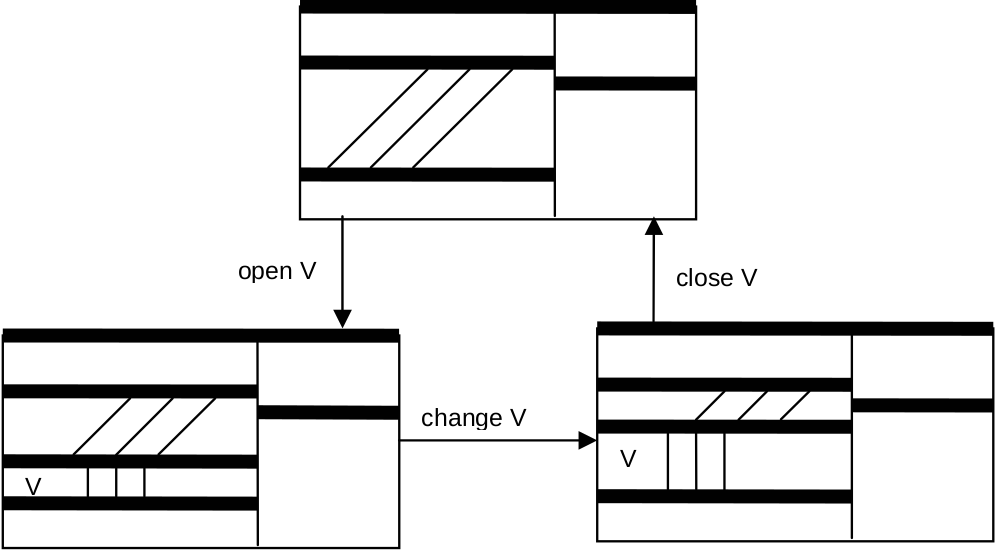
\includegraphics[width=.75\textwidth]{i/8}
  \caption{Basic operations on viewers}
  \label{fig:operation}
\end{figure}

The last group provides miscellaneous services.
\begin{itemize}
  \item \verb|This| identifies the viewer displayed at \verb|(X, Y)|.
  \item \verb|Next| returns the next upper neighbor of a given displayed viewer \verb|V|.
  \item \verb|Recall| allows recalling and restoring the most recently closed viewer.
  \item \verb|Locate| assists heuristic allocation of new viewers.
    For any given track and desired minimum height, it offers a choice
    of some distinguished viewers in this track:
    \begin{itemize}
      \item the \verb|fil|\textcolor{gray}{ler} viewer,
      \item the one at \verb|bot|\textcolor{gray}{tom},
      \item an \verb|alt|\textcolor{gray}{ernative} choice, and
      \item the viewer of \verb|max|\textcolor{gray}{imum} height.
    \end{itemize}
  \item Finally, \verb|Broadcast| broadcasts a message to the display area, that is,
    sends the given message to all currently displayed viewers.
\end{itemize}

It is now a good time to throw a glance behind the scenes.
Let us start with revealing \verb|Viewer| internal data structure.
Remember that according to the principle of information hiding
an internal data structure is fully private to the containing module
and accessible only through the module’s procedural interface.  Fig \ref{fig:snapshot}
shows a data structure view of the display snapshot taken in Fig \ref{fig:overlay}.
Note that the overlaid tracks and viewers are still part of the internal data structure.
\begin{figure}[h!]
  \centering
  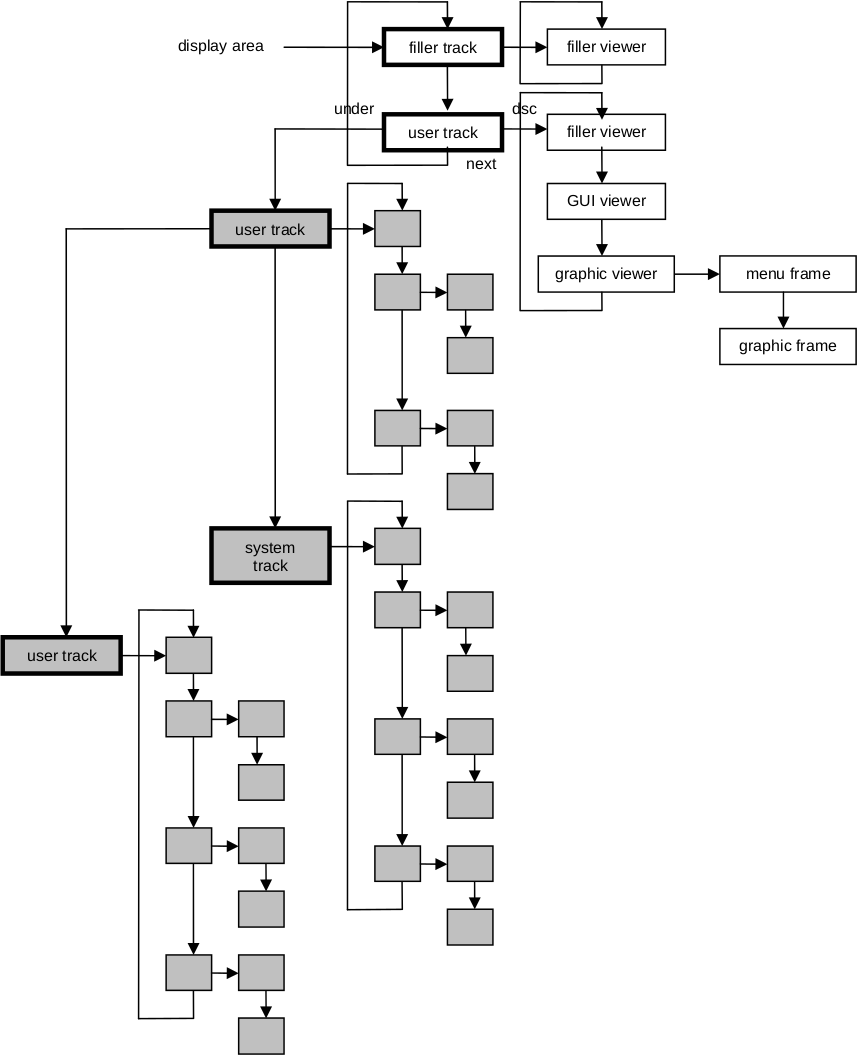
\includegraphics[width=\textwidth]{i/9}
  \caption{Internal data structure snapshot of Fig \ref{fig:overlay}}
  \label{fig:snapshot}
\end{figure}

In the data structure we recognize an anchor that represents the display area
and points to a list of tracks, each track pointing to a list of viewers,
each viewer in turn pointing to a list of arbitrary sub-frames.
Both the list of tracks and the list of viewers are closed to a ring,
where the filler track (filling up the display area)
and the filler viewers (filling up the tracks) act as anchors.
Additionally, each track points to a (possibly empty) list of tracks lying underneath.
These frames are invisible on the display, and shaded in Fig \ref{fig:snapshot}.

Technically, the track descriptor \verb|TrackDesc| is a private extension
of the viewer descriptor \verb|ViewerDesc|.
Repeating the declarations of viewer descriptors and frame descriptors,
we get to this hierarchy of types:
\begin{verbatim}
   TrackDesc = RECORD (ViewerDesc)
                      under: Display.Frame   END;

  ViewerDesc = RECORD (FrameDesc) state: INT END;

   FrameDesc = RECORD  next, dsc: Frame;
                      X, Y, W, H: INT;
                          handle: Handler    END;
\end{verbatim}

It is noteworthy that the data structure of the VM is heterogeneous with \verb|Frame| as base type.
It provides a nice example of a nested hierarchy of frames with the additional property
that the 1st 2 levels correspond to the 1st 2 levels in the type hierarchy defined by
\verb|Track|, \verb|Viewer|, and \verb|Frame|.

In an object-oriented environment objects are autonomous entities in principle.  However,
they may be bound to some higher instance (other than the system) temporarily.  For example,
we can look at the objects belonging to a module's private data structure as bound to this module.
Deciding if an object is currently bound then becomes a fundamental problem.  In the case of viewers,
this information is contained in an extra instance variable called \verb|state|.

As a system invariant, we have for every viewer $V$
\[ V\text{ is bound to module }Viewers \Leftrightarrow V.state \neq 0 \]
If we call any displayed viewer \emph{visible} and
each covered by an overlaying track \emph{suspended}, we can refine this invariant to
\begin{align*}
\{V\text{ is }&  visible\!\!\!\!\!\!\!\!\!\!\!\!\!\!\!\!\!\!\!\!\!\!\!\!\!\!\!&\Leftrightarrow V.state > 0\}&\text{ and }\\
\{V\text{ is }&suspended\!\!\!\!\!\!\!\!\!\!\!\!\!\!\!\!\!\!\!\!\!\!\!\!\!\!\!&\Leftrightarrow V.state < 0\}&
\end{align*}
In addition,
more detailed information about the kind of viewer $V$ is given by the magnitude $|V.state|$:
\begin{table}[h!]
  \centering
  \begin{tabular}{r l}
    $|V.state|$ & kind of viewer \\\hline
              0 & closed \\
              1 & filler \\
             -1 & productive
  \end{tabular}
\end{table}
\\The magnitude $|V.state|$ is kept invariant by \verb|Viewers|.
It could be used, for example, to distinguish different levels of importance or preference
with the aim of supporting a smarter algorithm for heuristic new viewers allocation.
$state$ is read-only to modules other than \verb|Viewers|.

We are now sufficiently prepared to understand how the exported \verb|Viewers| procedures
work behind.  They all operate on the internal dynamic data structure just explained.
\begin{itemize}
  \item \verb|This|, \verb|Next|, \verb|Locate|, \verb|Change| use it as a reference only
    or operate on individual elements
  \item \verb|InitTrack|, \verb|OpenTrack|, \verb|Open| add new elements, and
  \item \verb|CloseTrack|, \verb|Close| remove elements.
\end{itemize}
Most have side-effects on existing elements ($size$ or $state$).

Let us now change perspective and look at \verb|Viewers| as
a general low-level viewer manager (VMer) whose exact contents are unknown to it
(and whose controlling software might have been developed years later).
In short, let us look at \verb|Viewers| as a manager of black boxes.
Such an abstraction immediately makes it impossible for the implementation to call fixed procedures
for, say, changing a viewer's size or state.
The facility needed is a \emph{message-oriented interface}.
\begin{verbatim}
  TYPE ViewerMsg = RECORD (Display.FrameMsg) id,
                          X, Y, W, H, state: INT END;
\end{verbatim}

There're 3 variants of \verb|Viewer| messages, discriminated by \verb|id|:
\begin{table}[h!]
  \centering
  \begin{tabular}{l}
    restore contents, \\
    modify height (extend or reduce at bottom), and \\
    suspend (close temporarily or permanently).
  \end{tabular}
\end{table}
\\The additional components of the message inform about the desired new location, size, and state.
The following table lists senders, messages, and recipients of viewer messages.
\begin{table}[h!]
  \setlength{\tabcolsep}{1pt}
  \begin{tabular}{l|l|c r}
    \small{Originator} & \multicolumn{1}{c}{Message} & \multicolumn{2}{|c}{Recipients} \\\hline
    \small{OpenTrack}  & \small{suspend temporarily}
                       & \multicolumn{2}{l}{\small{viewers covered by opening track}} \\
    \small{CloseTrack} & \small{suspend permanently}
                       & \multicolumn{2}{l}{\small{viewers in closing track}}         \\
    \small{Open}       & \small{modify or suspend}
                       &        upper        &  opening viewer \\
    \small{Change}     & \small{modify}
                       & \small{neighbor of} & changing viewer \\
    \small{Close}      & \small{suspend permanently} & \multicolumn{2}{r}{closing viewer}
  \end{tabular}
\end{table}

\subsection{Menu Viewers}
\label{sub:menuviewers}
So far, we have treated viewers abstractly.
Next step we focus on a special class called \emph{menu viewers}.
From the earlier definition we know they're characterized by a structure
consisting of 2 vertically tiled \emph{descendant} frames,
\begin{table}[h!]
  \centering
  \begin{tabular}{r l}
    a frame of & at the \\\hline
    menu       & top, and \\
    contents   & bottom.
  \end{tabular}
\end{table}
\\Because the nature and contents of these frames are typically unknown
by their “ancestor” (or “parent”) viewer,
a collection of abstract messages is again a postulating form of interface.
As net effect, the handling of menu viewers boils down to a combination
of preprocessing, transforming and forwarding messages to the descendant frames.
In short, the display space is hierarchically organized and message passing within it
obeys the pattern of strict parental control.

Again, we start detailed discussion with module interface:
\begin{verbatim}
  DEFINITION MenuViewers;
    IMPORT Viewers, Display;        (*message ids*)
    CONST extend = 0; reduce = 1; move = 2;
    TYPE Viewer = POINTER TO ViewerDesc;
         ViewerDesc = RECORD (Viewers.ViewerDesc)
                             menuH: INT        END;
         ModifyMsg = RECORD (Display.FrameMsg)
                            id, dY, Y, H: INT  END;
  
    PROC Handle(       V: Display.Frame;
                   VAR M: Display.FrameMsg);

    PROC New(Menu , Main: Display.Frame;
             menuH, X, Y: INT             ): Viewer;
  END MenuViewers.
\end{verbatim}
The interface represented by this definition is conspicuously narrow.
There are just 2 procedures:
\begin{itemize}
  \item[a] generator procedure \verb|New|, and

    Returns a newly created menu viewer displaying the 2 (arbitrary) frames passed as parameters.

  \item[a] standard message handler \verb|Handle|.

    Implements the entire “behavior” of an object and in particular
    the above message dispatching functionality.
\end{itemize}

Message handlers in Oberon are implemented in the form of procedure variables that obviously
must be initialized properly at object creation time.  In other words, some concrete behavior
must explicitly be bound to each object, where different instances of the same object type
could potentially have a different behavior and/or the same instance could change its behavior
during its lifetime.  Our object model is therefore \emph{instance-centered}.

Conceptually, the creation of an object is an atomic action consisting of 3 basic steps:
\begin{enumerate}
  \item Allocate memory block;
  \item Install message handler;
  \item Initialize state variables.
\end{enumerate}
In the case of a standard menu \verb|V|\textcolor{gray}{iewer} creation:
\begin{verbatim}
  NEW(V); V.handle := Handle; V.dsc      := Menu;
          V.menuH  := menuH ; V.dsc.next := Main
\end{verbatim}
\verb|New| equals to \verb|create V; open V at X,Y|.
Opening \verb|V| needs \verb|Viewers|' assistance.

Implementing \verb|Handle| embodies the standard message handling strategy.
This is a coarse-grained view:
\begin{verbatim}
IF message reports about user interaction THEN
  IF variant is mouse tracking THEN
    IF mouse is in menu region THEN
      IF mouse is in upper menu region and
         left key is pressed THEN
        handle changing of viewer
      ELSE delegate handling to menu-frame
      END
    ELSE
      IF mouse is in main-frame THEN
        delegate handling to main-frame
      END
    END
  ELSIF variant is keyboard input THEN
    delegate handling to menu frame;
    delegate handling to main frame
  END

ELSIF message defines generic operation THEN
  IF message requests copy (clone) THEN
    send copy-message to menu frame to get a copy;
    send copy-message to main frame to get a copy;
    create menu viewer clone from copies
  ELSE
    delegate handling to menu frame;
    delegate handling to main frame
  END

ELSIF message reports about change of contents THEN
  delegate handling to menu frame;
  delegate handling to main frame

ELSIF message requests change of location/size THEN
  IF operation is restore THEN
    draw viewer area and border;
    send menu frm modify-msg to make extend from H 0;
    send main frm modify-msg to make extend from H 0
  ELSIF operation is modify THEN
    IF operation is extend THEN
      extend viewer area and border;
      send modify-msg to menu frm to make it extend;
      send modify-msg to main frm to make it extend
    ELSE (*reduce*)
      send modify-msg to main frm to make it reduce;
      send modify-msg to menu frm to make it reduce;
      reduce viewer area and border
    END
  ELSIF operation is suspend THEN
    send main frm modify-msg to make reduce to H 0;
    send menu frm modify-msg to make reduce to H 0
  END
END
\end{verbatim}

In principle, the handler acts as a message dispatcher that either processes a message directly
and/or delegates its processing to the descendant frames. Note that the handler's main alternative
statement discriminates precisely among the 4 basic categories of messages.

From the above outlined algorithm, handling copy messages, that is, requests for generating
a copy or clone of a menu viewer, we can derive a general recursive scheme for the creation
of a clone of an arbitrary frame:
\begin{enumerate}
  \item Send copy message to each element in the list of descendants;
  \item Generate copy of the original frame descriptor;
  \item Attach copies of descendants to the copy of descriptor.
\end{enumerate}

The essential point here is the use of new outgoing messages
in order to process a given incoming message.
We can regard message processing as a transformation
mapping incoming messages into a set of outgoing ones, with possible side-effects.
The simplest one, the input message being simply passed on to descendant(s),
is called \emph{delegation}.

As a fine point we clarify that the above algorithm is designed to create a deep copy
of a composite object (a menu viewer in our case).  If a shallow copy would be desired,
the descendants would not have to be copied, and the original descendants
instead of their copies would be attached to the copy of the composite object.

Another example of message handling is provided by mouse tracking.  Assume that
a mouse message is received by a menu viewer while the mouse is located in the upper part
of its menu frame and the left mouse key is kept down.  This means "change viewer's height
by moving its top line vertically".  No message to express the required transformation
of the sub-frames yet exists.  Consequently, module \verb|MenuViewer|s takes advantage of
our open (extensible) message model and simply introduces one called:
\begin{verbatim}
  ModifyMsg = RECORD (Display.FrameMsg)
                id, dY, Y, H: INT
              END;
\end{verbatim}
Field \verb|id| specifies one of the following 2 variants:
\begin{enumerate}
  \item \emph{extend}, or

    Requests the frame to move by the vertical translation vector \verb|dY|
    and then extend to height \verb|H| at bottom.

  \item \emph{reduce}.

    Requests the frame to reduce to height \verb|H| at bottom
    and then move by \verb|dY|.
\end{enumerate}
In both cases \verb|Y| indicates the Y-coordinate of the new lower-left corner.
Fig \ref{fig:modify} summarizes this graphically.
\begin{figure}[h!]
  \centering
  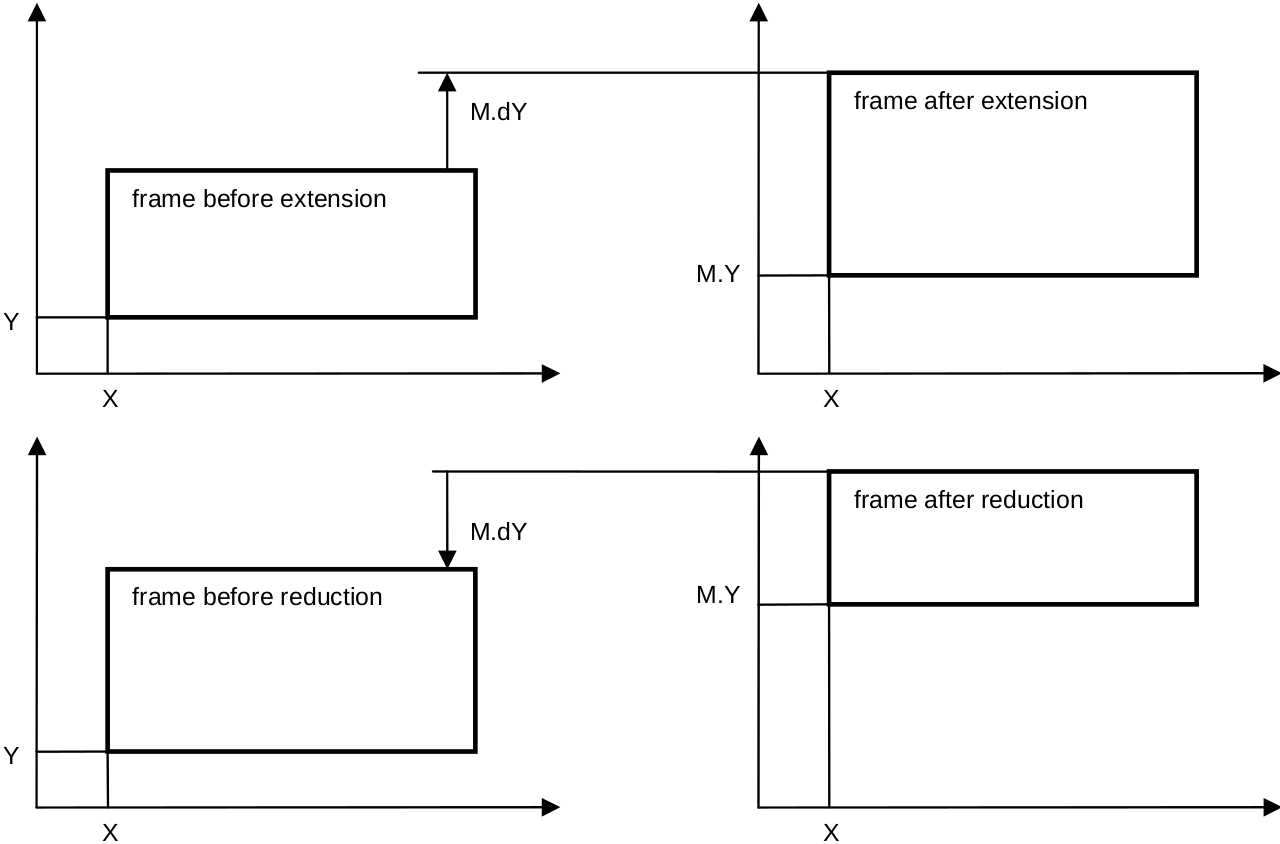
\includegraphics[width=.9\textwidth]{i/a}
  \caption{The modify frame operation}
  \label{fig:modify}
\end{figure}

Messages arriving from the VMer requesting the receiving viewer to extend or reduce
at its bottom are also mapped into \verb|ModifyMsg|s. Of course, no translation, $dY = 0$.

The attentive reader might perhaps have asked why the standard handler
is exported by \verb|MenuViewers| at all.  The thought behind is code reusability.
For example, a message handler for a subclass of menu viewers could be implemented effectively
by reusing menu viewer's standard one.  After having first handled all new or differing cases
it would simply (super-)call the standard handler subsequently.

\subsection{Cursor Management}
Traditionally, a cursor indicates and visualizes on the screen the current location of the caret
in a text or, more generally, the current \emph{focus of attention}.
A small arrow or similar graphic symbol is typically used for this purpose.
In Oberon, we have slightly generalized and abstracted this concept.
A cursor is a path in the logical display area whose current position can be made visible by a \emph{marker}.

The VMer and the cursor handler are 2 concurrent users of the same display area.
Actually, we should imagine 2 parallel planes,
\begin{table}[h!]
  \centering
  \begin{tabular}{r l}
              & displaying \\\hline
          one & viewers, and \\
    the other & cursors.
  \end{tabular}
\end{table}
\\If there's just 1 physical plane we take care of painting markers non-destructively, for example
in inverse-video mode.  Then, no precondition must be established before drawing a marker.
However, in the case of a viewer task painting destructively in its viewer's area,
the area must be locked first after turning invisible all markers in the area.

The technical support of cursor management is also contained in \verb|Oberon|.
The corresponding API:
\begin{verbatim}
DEFINITION Oberon;
  TYPE Marker = RECORD Fade,Draw: PROC(x,y: INT) END;
       Cursor = RECORD marker: Marker; X,Y: INT;
                                        on: BOOL END;
  VAR Arrow, Star   : Marker;
      Mouse, Pointer: Cursor;

  PROC OpenCursor(VAR c: Cursor);
  PROC FadeCursor(VAR c: Cursor);
  PROC DrawCursor(VAR c: Cursor;
                  VAR m: Marker; X, Y: INT);
  PROC MarkedViewer(): Viewers.Viewer;
  PROC RemoveMarks(X, Y, W, H: INT);
  ...
END Oberon.
\end{verbatim}
The state of a cursor is given by
\begin{table}[h!]
  \centering
  \begin{tabular}{r l}
    \verb|on|     & its mode of visibility, \\
    \verb|(X, Y)| & its position in the display area, and \\
    \verb|marker| & the current marker.
  \end{tabular}
\end{table}
\\\verb|Marker| is an abstract data type with an interface consisting of operations
  \verb|Fade| and
  \verb|Draw|.
The main benefit of this abstraction is once more conceptual independence
of the underlying hardware.  For example, they can
\begin{itemize}
  \item adapt to a given monitor hardware with built-in cursor support or,
    in case of absence of such support, simply
  \item be implemented as identical procedures (an involution)
    drawing the marker pattern in inverse video mode.
\end{itemize}

The functional interface to cursors consists of 3 operations:
\begin{table}[h!]
  \centering
  \begin{tabular}{l l}
    ~-\verb|Cursor| & to \\\hline
    \verb|Open| & open a new cursor, \\
    \verb|Fade| & switch off the marker of an open cursor, and \\
    \verb|Draw| & extend the path of a cursor to a new position \\
                & and mark it with the given marker.
  \end{tabular}
\end{table}
\\We emphasize that
the marker representing a given cursor can change its shape dynamically on the fly.

2 cursors are predefined:
\begin{table}[h!]
  \centering
  \begin{tabular}{r c l}
    cursor         & represents & \small{built-in }marker\small{ typically} \\\hline
    \verb|Mouse|   & the mouse  & \small{a small NW-pointing }\verb|Arrow| \\
    \verb|Pointer| &  a global  & \small{a }\verb|Star|\small{ symbol} \\
                   & \small{system pointer}
  \end{tabular}
\end{table}
\\The pointer can be used to mark any displayed object.
It serves primarily as an implicit parameter of commands.

2 assisting service procedures are added in connection with the predefined cursors:
\begin{table}[h!]
  \setlength{\tabcolsep}{3pt}
  \begin{tabular}{l|l}
    \verb|Marked| & \small{returns the viewer currently marked by the pointer,} \\
    \verb|-Viewer|& \small{equivalent to \verb|Viewers.This(Pointer.X, Pointer.Y)|.} \\\hline
    \verb|Remove| & \small{turns invisible within a given rectangle in display area,} \\
    \verb|-Marks| & \small{used to lock the rectangle for its caller.}
  \end{tabular}
\end{table}

Summary the essential concept points of cursor handling:
\begin{itemize}
  \item By virtue of the use of
    \begin{itemize}
      \item abstract markers, and
      \item the logical display area,
    \end{itemize}
    any potential hardware dependence is encapsulated in system modules
    and is therefore hidden from the application programmer.
    Cursors are moving uniformly within the whole display area,
    even across screen boundaries.

  \item Cursor handling is decentralized by delegating it to the individual handlers
    that are installed in viewers.  Typically, a handler reacts on the receipt
    of a mouse tracking message by drawing the mouse cursor at the indicated new position.
    The benefit of such individualized handling is flexibility.  For example,
    a smart local handler might choose the shape of the visualizing marker
    depending on the exact location, or it might force the cursor onto a grid point.

  \item Even though cursor handling is decentralized, there is some intrinsic support
    for cursor drawing built into the \verb|Cursor| declaration.
    Cursors are full value objects and, as such, can "memorize" their current state.
    Consequently, the interface operations \verb|FadeCursor| and \verb|DrawCursor|
    need to refer to the desired future state only.

  \item Looking at the VMer as one user of the display area, the cursor handler
    is the 2nd (and logically concurrent) user of the same resource.  If there is
    just one physical plane implementing the display area, any region must be locked
    by a current user before destructive painting.  Therefore,
    markers are usually painted non-destructively in inverse-video mode.
\end{itemize}

Let us now recapitulate the entire section.
\begin{itemize}
  \item The central resource managed by the display subsystem is the \emph{logical display area}
    whose purpose is abstraction from the underlying display monitor hardware.

    The display area is primarily used by the VMer for the accommodation of tracks and viewers,
    which are merely the 1st 2 levels of a potentially unlimited nested hierarchy of display frames.
    For example, standard menu viewers contain 2 subordinate frames:
    \begin{itemize}
      \item a menu frame, and
      \item a main frame of contents.
    \end{itemize}

  \item Viewers are treated as black boxes by the VMer and are addressed via messages.

    Viewers and, more generally frames, are used as elements of \emph{message-based interfaces}
    connecting the display subsystem with other subsystems like
    \begin{itemize}
      \item the task scheduler, and
      \item the various document managers.
    \end{itemize}

  \item Finally, the display area is also the living room of cursors.  In Oberon,
    a cursor is a marked path, 2 standard cursors \verb|Mouse| and \verb|Pointer| are predefined.
\end{itemize}

\chapter{Statements and Expressions}
The specification of an action is called a statement. Statements can be interpreted (executed), and
that interpretation (execution) has an effect. The effect is a transformation of the state of the
computation, the state being represented by the collective values of the program's variables. The most
elementary action is the assignment of a value to a variable. The assignment statement has the form
\begin{verbatim}
  assignment = designator ":=" expression.
\end{verbatim}
and its corresponding action consists of 3 parts in this sequence:
\begin{enumerate}
  \item Evaluate the designator designating a variable.
  \item Evaluate the expression yielding a value.
  \item Replace the value of the variable identified in 1. by the value obtained in 2.
\end{enumerate}
Simple examples of assignments are:
\begin{verbatim}
  i := 1    x := y+z
\end{verbatim}
Here $i$ obtains the value 1, and $x$ the sum of $y$ and $z$, and the previous values are lost.
Evidently, every variable in an expression must previously have been assigned a value. Observe that
the following pairs of statements, executed in sequence, do not have the same effect:
\begin{verbatim}
  i := i+1; j := 2*i
  j := 2*i; i := i+1
\end{verbatim}
Assuming the initial value $i = 0$, the 1st pair yields $i = 1$, $j = 2$, whereas the 2nd pair yields
$j = 0$.  If we wish to exchange the values of variables $i$ and $j$, the statement sequence
\begin{verbatim}
  i := j; j := i
\end{verbatim}
will not have the desired effect. We must introduce a temporary value holder, say $k$, and specify
the 3 consecutive assignments
\begin{verbatim}
  k := i; i := j; j := k
\end{verbatim}
An expression is in general composed of several operands and operators. Its evaluation consists of
applying the operators to the operands in a prescribed sequence, in general taking the operators
from left to right. The operands may be constants, or variables, or functions. (The latter will be
explained in a later chapter.) The identification of a variable will, in general, again require the
evaluation of a designator. Here we shall confine our presentation to simple variables designated
by an identifier. Arithmetic expressions (there exist other expressions too) involve numbers,
numeric variables, and arithmetic operators. These include the basic operations of addition (+),
subtraction (-), multiplication (*), and division. They will be discussed in detail in the chapter on
basic data types. Here it may suffice to mention that the slash (/) is reserved for dividing real
numbers, and that for integers we use the operator DIV which truncates the quotient.

An expression consists of consecutive terms. The expression
\begin{verbatim}
  T0 + T1 + ... + Tn
\end{verbatim}
is equivalent to
\begin{verbatim}
  ((T0 + T1) + ...) + Tn
\end{verbatim}
and is syntactically defined by the rules
\begin{verbatim}
  SimpleExpression =[+|-] term {AddOperator term}.
  AddOperator = + | - | OR
\end{verbatim}

\textbf{Note}: for the time being, the reader may consider the syntactic entities expression and
SimpleExpression as equivalent. Their difference and the operators OR, AND, and NOT will be
explained in the chapter on the data type BOOL.

Each term similarly consists of factors. The term
\begin{verbatim}
  F0 * F1 * ... * Fn
\end{verbatim}
is equivalent to
\begin{verbatim}
  ((F0 * F1) * ... ) * Fn
\end{verbatim}
and is syntactically defined by the rules
\begin{verbatim}
  term = factor {MulOperator factor}.
  MulOperator = * | / | DIV | MOD | &.
\end{verbatim}
Each factor is either a constant, a variable, a function, or an expression itself enclosed by
parentheses.

Examples of (arithmetic) expressions are
\begin{verbatim}
  2*3 + 4*5       = (2*3)+(4*5)   = 26
  15 DIV 4 * 4    = (15 DIV 4)*4  = 12
  15 DIV (4*4)    = 15 DIV 16     = 0
  2 + 3*4 - 5     = 2 + (3*4) - 5 = 9
  6.25/1.25 + 1.5 = 5.0 + 1.5     = 6.5
\end{verbatim}
The syntax of factors, implying that a factor may itself be an expression, is evidently recursive. The
general form of designators will be explained later; here it suffices to know that an identifier
denoting a variable or a constant is a designator.
\begin{verbatim}
  factor = number | string | set | designator
    [ActualParameters] | (expression) | ~factor.
\end{verbatim}
The rules governing expressions are actually quite simple, and complicated expressions are rarely
used. Nevertheless, we must point out a few basic rules that are well worth remembering.
\begin{enumerate}
  \item Every variable in an expression must previously have been assigned a value.
  \item 2 operators must never be written side by side. For instance \verb|a * -b| is illegal and
    must be written as \verb|a*(-b)|.
  \item The multiplication sign must never be omitted when a multiplication is required. For
    example, \verb|2n| is illegal and must be written as \verb|2*n|.
  \item MulOperators are binding more strongly than AddOperators.
  \item When in doubt about evaluation rules (i.e. precedence of operators), use additional
    parentheses to clarify. For example, \verb|a+b*c| may just as well be written as
    \verb|a+(b*c)|.
\end{enumerate}
The assignment is but one of the possible forms of statements. Other forms will be introduced in the
following chapters. We enumerate these forms by the following syntactic definition
\begin{verbatim}
  statement = [ assignment | ProcedureCall | IfStatement
    | WhileStatement | RepeatStatement | ForStatement ].
\end{verbatim}
Several of these forms are structured statements, i.e. some of their components may be statements
again. Hence, the definition of statement is, like that of expressions, recursive.

The most basic structure is the sequence. A computation is a sequence of actions, where each
action is specified by a statement, and is executed after the preceding action is completed. This
strict sequentiality in time is an essential assumption of sequential programming. If a statement
$S_1$ follows $S_0$, then we indicate this sequentiality by a semicolon
\[  S_0; S_1 \]
This statement separator (not terminator) indicates that the action specified by $S_0$ is to be
followed immediately by the action corresponding to $S_1$. A sequence of statements is syntactically
defined as
\begin{verbatim}
  StatementSequence = statement {; statement}.
\end{verbatim}
The syntax of statements implies that a statement may consist of no symbols at all. In this case, the
statement is said to be empty and evidently denotes the null action. This curiosity among statements
has a definite reason: it allows semicolons to be inserted at places where they are actually
superfluous, such as at the end of a statement sequence.

\chapter{Control Structures}
It is a prime characteristic of computers that individual actions can be selected, repeated, or
performed conditionally depending on some previously computed results. Hence the sequence of
actions performed is not always identical with the sequence of their corresponding statements. The
sequence of actions is determined by control structures indicating repetition, selection, or
conditional execution of given statements.

\section{Repetitive Statements}
The most common situation is the repetition of a statement or statement sequence under control of
a condition: the repetition continues as long as the condition is met. This is expressed by the 
\emph{while statement}. Its syntax is
\begin{verbatim}
  WhileStatement = WHILE expr DO StatementSequence END
\end{verbatim}
and its corresponding action is:
\begin{enumerate}
  \item Evaluate the condition which takes the form of an expression yielding
    the value \verb|TRUE| or \verb|FALSE|;
  \item If the value is \verb|TRUE|, execute the statement sequence and then repeat with step 1;
    if the value is \verb|FALSE|, terminate.
\end{enumerate}
The expression is of type \verb|BOOL|. This will be further discussed in the chapter on data types.
Here it suffices to know that a simple comparison is a Boolean expression. An example was given
in the introductory example, where repetition terminates when the 2 comparands have become
equal. Further examples involving while statements are:
\begin{enumerate}
  \item Initially, let $q = 0$ and $r = x$; then count the number of times $y$ can be subtracted
    from $x$, i.e. compute the quotient $q = x$\verb| DIV |$y$, and remainder $r = x$\verb| MOD |$y$,
    if $x$ and $y$ are natural numbers.
    \begin{verbatim}
      WHILE r >= y DO r := r-y; q := q+1 END
    \end{verbatim}
  \item Initially, let $z = 1$ and $i = k$; then multiply $z$ $k$ times by $x$, i.e. compute
    $z = xk$, if z and k are natural numbers:
    \begin{verbatim}
      WHILE i > 0 DO z := z*x; i := i-1 END
    \end{verbatim}
\end{enumerate}
When dealing with repetitions, it is important to remember the following points:
\begin{enumerate}
  \item During each repetition, progress must be made towards meeting the goal, namely "getting
    closer" to satisfying the termination condition. An obvious corollary is that the condition
    must be somehow affected from within the repeated computation. The following statements are
    either incorrect or dependent on some critical precondition as stated.
    \begin{verbatim}
      WHILE i > 0 DO
        k := 2*k (*i is not changed*)
      END
 
      WHILE i # 0 DO
        i := 1-2 (*i must be even and positive*)
      END
 
      WHILE n # i DO
        n := n*i; i := i+1
      END
    \end{verbatim}
  \item If the condition is not satisfied initially, the statement is vacuous, i.e. no action
    is performed.

  \item In order to obtain a grasp of the effect of the repetition, we need to establish a
    relationship that is stable, called an invariant. In the division example above, this is the
    equation $q*y + r = x$ holding each time the repetition is started. In the exponentiation
    example it is $z * x^i = x^k$ which, together with the termination condition $i = 0$ yields
    the desired result $z = x^k$.

  \item The repetition of identical computations should be avoided (although a computer has
    infinite patience and will not complain). A simple rule is to avoid expressions within
    repetitive statements, in which no variable changes its value. For example, the statement
    \begin{verbatim}
      WHILE i < 3*N DO tab[i] := x + y*z + z*i;
                       i := i+1 END
    \end{verbatim}
    should be formulated more effectively as
    \begin{verbatim}
      n := 3*N; u := x + y*z;
      WHILE i < n DO tab[i] := u + z*i; i := i+1 END
    \end{verbatim}
\end{enumerate}

In addition to the while statement, there is the \emph{repeat statement}, syntactically defined as
\begin{verbatim}
  RepeatStatement = REPEAT StatementSequence UNTIL expr
\end{verbatim}
The essential difference to the while statement is that the termination condition is checked each
time after (instead of before) execution of the statement sequence. As a result, the sequence is
executed at least once. An advantage is that the condition may involve variables that are undefined
when the repetition is started.
\begin{verbatim}
  REPEAT i := i+5; j := j+7; k := i DIV j UNTIL k > 23
  REPEAT r := r-y; q := q+1 UNTIL r < y
\end{verbatim}

\section{Conditional Statements}
The conditional statement, also called if statement, has the form
\begin{verbatim}
IfStatement = IF expr THEN StatementSequence
          {ELSIF expr THEN StatementSequence}
                     [ELSE StatementSequence]
              END
\end{verbatim}
The following example illustrates its general form.
\begin{verbatim}
     IF R1 THEN S1
  ELSIF R2 THEN S2
  ELSIF R3 THEN S3
           ELSE S4 END
\end{verbatim}
The meaning is obvious from the wording. However, it must be remembered that the expressions
\verb|R1 ... R3| are evaluated one after the other, and that as soon as one yields the value
\verb|TRUE|, its corresponding statement sequence is executed, whereafter the \verb|IF| statement
is considered as completed. No further conditions are tested. Examples are:
\begin{verbatim}
     IF x = 0 THEN s :=  0
  ELSIF x < 0 THEN s := -1
              ELSE s :=  1 END

  IF ODD(k) THEN z := z*x END
  IF k > 10 THEN k := k-10; d := 1
            ELSE d := 0 END
\end{verbatim}

The constructs discussed so far enable us to develop a few simple, complete programs as
subsequently described. The 1st example is an extension of our introductory example computing
the greatest common divisor $gcd$ of 2 natural numbers $x$ and $y$. The extension consists in
the addition of 2 variables $u$ and $v$, and statements which lead to the computation of the
least common multiple $lcm$ of $x$ and $y$. The $lcm$ and $gcd$ are related by the equation
\begin{verbatim}
  lcm(x,y) * gcd(x,y) = x*y
\end{verbatim}

As explained earlier, this and following examples will be formulated as command procedures and
are assumed to be embedded in module \verb|Pattern| defined in \ref{ch:1ex} which imports
modules \verb|Texts| and \verb|Oberon|.
\begin{verbatim}
  PROC gcdlcm*;
    VAR x, y, u, v: INT; S: Texts.Scanner;
  BEGIN Texts.OpenScanner(S, Oberon.Par.text,
                             Oberon.Par.pos):
    Texts.Scan(S); x := S.i;
    Texts.WriteString(W, " x =");
    Texts.WriteInt(W, x, 6);
    Texts.Scan(S); y := S.i;
    Texts.WriteString(W, " y =");
    Texts.WriteInt(W, y, 6);
    u := x; v := y;
    (*gcd(x,y) = gcd(x0,yO), x*v + y*u = 2*x0*y0*)
    WHILE x # y DO
      IF x > y THEN x := x-y; u := u+v
               ELSE y := y-x; v := v+u
      END
    END;
    Texts.WriteInt(W, x, 6);
    Texts.WriteInt(W, (u+v) DIV 2, 6);
    Texts.WriteLn(W);
    Texts.Append(Oberon.Log, W.buf)
  END gcdlcm.
\end{verbatim}
This example again shows the nesting of control structures. The repetition expressed by a while
statement includes a conditional structure expressed by an if statement, which in turn includes
2 statement sequences, each consisting of 2 assignments. This hierarchical structure is made
transparent by appropriate indentation of the "inner" parts.

Another example demonstrating a hierarchical structure computes the real number $x$ raised to
the power $i$, where $i$ is a non-negative integer.
\begin{verbatim}
  PROC Power*;
    VAR i: INT; x, z: REAL; S: Texts.Scanner;
  BEGIN Texts.OpenScanner(S, Oberon.Par.text,
                             Oberon.Par.pos);
    Texts.Scan(S);
    WHILE S.class = Texts.Real DO
      x := S.x; Texts.WriteString(W, " x =");
      Texts.WriteReal(W, x, 16); Texts.Scan(S);
      i := S.i; Texts.WriteString(W, " i =");
      Texts.WriteInt(W, i, 4);
      z= 1.0:
      (* z * x^i = x0^i0 *)
      WHILE i > 0 DO z := z*x; i := i-1 END;
      Texts.WriteReal(W, z, 16);
      Texts.WriteLn(W); Texts.Scan(S)
    END;
    Texts.Append(Oberon.Log, W.buf)
  END Power.
\end{verbatim}
Here we subject the computation to yet another repetition: Each time a result has been computed,
another value pair $x, i$ is requested. This outermost repetition is controlled by the relation
\verb|S.class = Texts.Real|, which indicates whether a real number $x$ had actually been read.
As an example, activation of the command
\begin{verbatim}
  M.Power 5.0 2   2.0 5   3.0 3 ~
\end{verbatim}
will generate the results \verb|25.0, 32.0, 27.0|.

The straight-forward computation of a power by repeated multiplication is, although obviously
correct, not the most economical. We now present a more sophisticated and more efficient solution.
It is based on the following consideration: The goal of the repetition is to reach the value $i = 0$.
This is done by successively reducing $i$, while maintaining the invariant $z * x^i = x_0^{i_0}$,
where $x_0$ and $i_0$ denote the initial values of $x$ and $i$. A faster algorithm therefore must
rely on decreasing $i$ in larger steps. The solution given here halves $i$. But this is only possible,
if $i$ is even. Hence, if $i$ is odd, it is 1st decremented by 1. Of course, each change of $i$ must
be accompanied by a corrective action on $z$ in order to maintain the invariant.
\begin{itemize}
  \item A detail: the subtraction of 1 from $i$ is not expressed by an explicit statement, because
    it is performed implicitly by the subsequent division by 2.
  \item 2 further details are noteworthy:
  \begin{enumerate}
    \item The function \verb|ODD(i)| is \verb|TRUE|, if $i$ is an odd number, \verb|FALSE| otherwise.
    \item $x$ and $z$ denote real values, as opposed to integer values. Hence, they can represent
      fractions, too.
  \end{enumerate}
\end{itemize}
\begin{verbatim}
  PROC Power*;
    VAR i: INT; x, z: REAL; S: Texts.Scanner;
  BEGIN Texts.OpenScanner(S, Oberon.Par.text,
                             Oberon.Par.pos);
    Texts.Scan(S);
    WHILE S.class = Texts.Real DO
      x := S.x; Texts.WriteString(W, " x =");
      Texts.WriteReal(W, x, 16): Texts.Scan(S);
      i := S.i; Texts.WriteString(W, " i=");
      Texts.WriteInt(W, i, 4);
      z := 1.0;
      WHILE i > 0 DO
        (* z* x^i = x0^i0 *)
        IF ODD(i) THEN z := z*x END;
        x := x*x; i := i DIV 2
      END;
      Texts.WriteReal(W, z, 16);
      Texts.WriteLn(VW); Texts.Scan(S)
    END;
    Texts.Append(Oberon.Log, W.buf)
  END Power.
\end{verbatim}

The next sample command has a structure that is almost identical to the preceding program. It
computes the logarithm of a real number $x$ whose value lies between 1 and 2. The invariant in
conjunction with the termination condition ($b=0$) implies the desired result $sum=\log_2{x}$.
\begin{verbatim}
  PROC Log2*;
    VAR x, a, b, sum: REAL; S: Texts.Scanner;
  BEGIN Texts.OpenScanner(S, Oberon.Par.text,
                             Oberon.Par.pos);
    Texts.Scan(S);
    WHILE S.class = Texts.Real DO
      x := S.x; Texts.WriteReal(W, x, 15); (*1<=x<2*)
      a :=x; b := 1.0; sum := 0.0;
      REPEAT (*log_2(x) = sum + b*log_2(a)*)
        a := a*a; b := 0.5*b;
        IF a >= 2.0 THEN
          sum := sum + b; a := 0.5*a
        END
      UNTIL b < 1.0E-7;
      Texts.WriteReal(W, sum, 16);
      Texts.WriteLn(W); Texts.Scan(S)
    END;
    Texts.Append(Oberon.Log, W.buf)
  END Log2.
\end{verbatim}

Normally, routines for computing standard mathematical functions need not be programmed in
detail, because they are available from a collection of modules similar to those for input
and output. Such a collection is, somewhat inappropriately, called a library. In the following
example, again exhibiting the use of a repetitive statement, we use routines for computing the
cosine and the exponential function from a library called Math and generate a table of values
for a damped oscillation. Typically, the available standard routines include the $sin$, $cos$,
$exp$, $ln$ (logarithm), $sqrt$ (square root), and the $arctan$ functions.
\begin{verbatim}
  PROC Oscillation*;
    CONST dx = 0.19634953; (*pi/16*)
    VAR i, n: INT; x, y, REAL; S: Texts.Scanner;
  BEGIN Texts.OpenScanner(S, Oberon.Par.text,
                             Oberon.Par.pos):
    Texts.Scan(S); n := S.i; Texts.WriteInt(W, n, 6);
    Texts.Scan(S); r := S.x; Texts.WriteReal(W, r, 15);
    Texts.WriteLn(W); i := 0; x := 0.0;
    REPEAT x := x + dx; i := i+1;
           y := Math.exp(-r*x) * Math.cos(x);
           Texts.WriteReal(W, x, 15);
	   Texts.WriteReal(W, y, 15);
	   Texts.WriteLn(W)
    UNTIL i >= n;
    Texts.Append(Oberon.Log, W.buf)
  END Oscillation.
\end{verbatim}

\chapter{Text}
\label{ch:text}
At the beginning of the computing era, text was the only medium mediating information
between users and computers.  Not only was a textual notation used to denote
all kinds of data and objects via names and numbers
(represented by sequences of characters and digits respectively),
but also for the specification of programs
(based on the notions of formal language and syntax) and tasks.
Actually, not even the most modern and most sophisticated computing environments
have been able to make falter the dominating role of text substantially.
At most, they have introduced alternative models like graphical user interfaces (GUI)
as a graphical replacement for \emph{command lines}.

There are many reasons for the popularity of text in general
and in connection with computers in particular.  To name but a few:
\begin{itemize}
  \item Text containing any arbitrary amount of information can be built
    from a small alphabet of widely standardized elements (characters),
  \item their building pattern is extremely simple (lining up elements), and
  \item the resulting structure is most elementary (a sequence).
\end{itemize}
And perhaps most importantly, \emph{syntactically structured text
can be parsed and interpreted by a machine}.

In computing terminology, sequences of elements are called \emph{files} and,
in particular, sequences of characters are known as \emph{text files}.
Looking at their binary representation, we find text files excellently suited
to be stored in computer memories and on external media.
Remember that individual characters are usually encoded in 1 byte each (ASCII).
We can therefore identify the binary structure of text files with sequences of bytes,
matching perfectly the structure of any underlying computer storage.
We should recall at this point that, with the possible exception of line-break control characters,
rendering information is not part of ordinary text files.
For example, the choices of character style and of paragraph formatting parameters
are entirely left to the rendering interpreter.

Unfortunately, in conventional computing environments, text is merely used for input/output,
and its potential is not nearly exploited optimally.
Input texts are typically read from the keyboard under control of some text editor,
interpreted and then discarded.  Output text is volatile.
Once displayed on the screen it is no longer available to any other parts of the program.
The root of the problem is easily located:
Conventional OSes neither feature an integrated management
nor an abstract programming interface (PI) for texts.

Of course,
such poor support of text on the level of programming must reflect itself on the user surface.
More often than not, users are forced to retype a certain piece of text
instead of simply copy/pasting it from elsewhere on the screen.
Investigations have shown that, in average,
up to 80\% of required input text is already displayed somewhere.

Motivated by our positive experience with integrated text in the Cedar system \cite{Teitelman}
we decided to provide a central text management in Oberon at a sufficiently low system level.
However, this is not enough.  We actually need an abstract PI for text, that is,
an abstract data type \verb|Text|, together with a complete set of operations.
We shall devote \ref{sec:textyp} to the explanation of this data type.
In \ref{sec:textmanagement}, we take a closer look at the basic text management,
including data structures and algorithms used for the implementation of type \verb|Text|.

Text frames are a special class of display frames.  They appear typically (but not necessarily)
as frames within a menu viewer (see \ref{sub:menuviewers}).  Their role is double-faced:
\begin{itemize}
  \item[a)] Rendering text on the display screen, and
  \item[b)] interpreting interactive editing commands.
\end{itemize}
The details will be discussed in \ref{sec:textframes}.

With the aim of exploiting the power of modern bitmap-displays
and also of reusing the results of earlier projects in the field of digital font design,
we decided in favor of supporting “rich texts” in Oberon, including graphical attributes
and in particular font specification.  In \ref{sec:fontmachinery} we shall explain the font machinery,
starting from an abstract level and proceeding down to the level of raster data.

\chapter{Overview}
\section{History \& Motivation}
How could anyone diligently concentrate on his work in an afternoon with such warmth, splendid
sunshine, and blue sky. This rhetorical question was one I asked many times while spending a
sabbatical leave in California in 1985. Back home everyone would feel compelled to profit from the
sunny spells to enjoy life at leisure in the country-side, wandering or engaging in one's favourite
sport. But here, every day was like that, and giving in to such temptations would have meant the
end of all work. And, had I not chosen this location in the world because of its inviting, enjoyable climate?

Fortunately, my work was also enticing, making it easier to buckle down. I had the privilege of
sitting in front of the most advanced and powerful workstation anywhere, learning the secrets of
perhaps the newest fad in our fast developing trade, pushing colored rectangles from one place of
the screen to another. This all had to happen under strict observance of rules imposed by physical
laws and by the newest technology. Fortunately, the advanced computer would complain
immediately if such a rule was violated, it was a rule checker and acted like your big brother,
preventing you from making steps towards disaster. And it did what would have been impossible for
oneself, keeping track of thousands of constraints among the thousands of rectangles laid out. This
was called computer-aided design. "Aided" is rather a euphemism, but the computer did not
complain about the degradation of its role.

While my eyes were glued to the colorful display, and while I was confronted with the evidence of
my latest inadequacy, in through the always open door stepped my colleague (JG). He also
happened to spend a leave from duties at home at the same laboratory, yet his face did not exactly
express happiness, but rather frustration. The chocolate bar in his hand did for him what the coffee
cup or the pipe does for others, providing temporary relaxation and distraction. It was not the first
time he appeared in this mood, and without words I guessed its cause. And the episode would
reoccur many times.

His days were not filled with the great fun of rectangle-pushing; he had an assignment. He was
charged with the design of a compiler for the same advanced computer. Therefore, he was forced
to deal much more closely, if not intimately, with the underlying software system. Its rather frequent
failures had to be understood in his case, for he was programming, whereas I was only using it
through an application; in short, I was an end-user! These failures had to be understood not for
purposes of correction, but in order to find ways to avoid them. How was the necessary insight to
be obtained? I realized at this moment that I had so far avoided this question; I had limited
familiarization with this novel system to the bare necessities which sufficed for the task on my mind.

It soon became clear that a study of the system was nearly impossible. Its dimensions were simply
awesome, and documentation accordingly sparse. Answers to questions that were momentarily
pressing could best be obtained by interviewing the system's designers, who all were in-house. In
doing so, we made the shocking discovery that often we could not understand their language.
Explanations were fraught with jargon and references to other parts of the system which had
remained equally enigmatic to us.

So, our frustration-triggered breaks from compiler construction and chip design became devoted to
attempts to identify the essence, the foundations of the system's novel aspects. What made it
different from conventional OSes? Which of these concepts were essential, which
ones could be improved, simplified, or even discarded? And where were they rooted? Could the
system's essence be distilled and extracted, like in a chemical process?

During the ensuing discussions, the idea emerged slowly to undertake our own design. And
suddenly it had become concrete. "Crazy" was my first reaction, and "impossible". The sheer
amount of work appeared as overwhelming. After all, we both had to carry our share of teaching
duties back home. But the thought was implanted and continued to occupy our minds.

Sometime thereafter, events back home suggested that I should take over the important course
about System Software. As it was the unwritten rule that it should primarily deal with operating
system principles, I hesitated. My scruples were easily justified: After all I had never designed such
a system nor a part of it. And how can one teach an engineering subject without first-hand experience?

Impossible? Had we not designed compilers, OSes, and document editors in small
teams? And had I not repeatedly experienced that an inadequate and frustrating program could be
programmed from scratch in a fraction of source code used by the original design? Our brainstorming
continued, with many intermissions, over several weeks, and certain shapes of a system
structure slowly emerged through the haze. After some time, the preposterous decision was made:
we would embark on the design of an OS for our workstation (which happened to be
much less powerful than the one used for my rectangle-pushing) from scratch.

The primary goal, to personally obtain first-hand experience, and to reach full understanding of
every detail, inherently determined our manpower: two part-time programmers. We tentatively set
our time-limit for completion to three years. As it later turned out, this had been a good estimate;
programming was begun in early 1986, and a first version of the system was released in the fall of 1988.

Although the search for an appropriate name for a project is usually a minor problem and often left
to chance and whim of the designers, this may be the place to recount how Oberon entered the
picture in our case. It happened that around the time of the beginning of our effort, the space probe
Voyager made headlines with a series of spectacular pictures taken of the planet Uranus and of its
moons, the largest of which is named Oberon. Since its launch I had considered the Voyager
project as a singularly well-planned and successful endeavor, and as a small tribute to it I picked
the name of its latest object of investigation. There are indeed very few engineering projects whose
products perform way beyond expectations and beyond their anticipated lifetime; mostly they fail
much earlier, particularly in the domain of software. And, last but not least, we recall that Oberon is
famous as the king of elfs.

The consciously planned shortage of manpower enforced a single, but healthy, guideline:
Concentrate on essential functions and omit embellishments that merely cater to established
conventions and passing tastes. Of course, the essential core had first to be recognized and
crystallized. But the basis had been laid. The ground rule became even more crucial when we
decided that the result should be able to be used as teaching material. I remembered C.A.R. Hoare's
plea that books should be written presenting actually operational systems rather than half baked,
 abstract principles. He had complained in the early 1970s that in our field engineers were
told to constantly create new artifacts without being given the chance to study previous works that
had proven their worth in the field. How right was he, even to the present day!

The emerging goal to publish the result with all its details let the choice of programming language
appear in a new light: it became crucial. Modula-2 which we had planned to use, appeared as not
quite satisfactory. Firstly, it lacked a facility to express extensibility in an adequate way. And we had
put extensibility among the principal properties of the new system. By "adequate" we include
machine-independence. Our programs should be expressed in a manner that makes no reference
to machine peculiarities and low-level programming facilities, perhaps with the exception of device
interfaces, where dependence is inherent.

Hence, Modula-2 was extended with a feature that is now known as type extension. We also
recognized that Modula-2 contained several facilities that we would not need, that do not genuinely
contribute to its power of expression, but at the same time increase the complexity of the compiler.
But the compiler would not only have to be implemented, but also to be described, studied, and
understood. This led to the decision to start from a clean slate also in the domain of language
design, and to apply the same principle to it: concentrate on the essential, purge the rest. The new
language, which still bears much resemblance to Modula-2, was given the same name as the
system: Oberon [1, 2]. In contrast to its ancestor it is terser and, above all, a significant step
towards expressing programs on a high level of abstraction without reference to machine-specific
features.

We started designing the system in late fall 1985, and programming in early 1986. As a vehicle we
used our workstation Lilith and its language Modula-2. First, a cross-compiler was developed, then
followed the modules of the inner core together with the necessary testing and down-loading
facilities. The development of the display and the text system proceeded simultaneously, without
the possibility of testing, of course. We learned how the absence of a debugger, and even more so
the absence of a compiler, can contribute to careful programming.

Thereafter followed the translation of the compiler into Oberon. This was swiftly done, because the
original had been written with anticipation of the later translation. After its availability on the target
computer Ceres, together with the operability of the text editing facility, the umbilical cord to Lilith
could be cut off. The Oberon had become real, at least its draft version. This happened
around the middle of 1987; its description was published thereafter [3], and a manual and guide
followed in 1991 [5].

The system's completion took another year and concentrated on connecting the workstations in a
network for file transfer [4], on a central printing facility, and on maintenance tools. The goal of
completing the system within three years had been met. The system was introduced in the middle
of 1988 to a wider user community, and work on applications could start. A service for electronic
mail was developed, a graphics system was added, and various efforts for general document
preparation systems proceeded. The display facility was extended to accommodate two screens,
including color. At the same time, feedback from experience in its use was incorporated by
improving existing parts. Since 1989, Oberon has replaced Modula-2 in our introductory programming courses.

\section{Overview}
This book consists of 3 main parts, excluding this preface and overview(PO) part:
\begin{enumerate}
	\item OS
	\item apps
	\item hardware computer
\end{enumerate}

First, OS. Implementation of a system proceeds bottom-up naturally, because higher level modules are
clients of those lower level and cannot function without their imports. Description, on the contrary,
should better be arranged in the reverse top-down way. This is because a system is designed with its
expected applications and functions in mind. Decomposition into a hierarchy of modules is justified by
the use of auxiliary functions and abstractions, or by postponing more detailed explanation later, when the need has been fully motivated. Thus, we will describe the OS part top-down essentially.

\ref{ch:struct} first explains the most important basic concepts like Viewers, Commands, Tasks and Texts, etc. which will be further elaborated in the following chapters. It ends with the system structure, to share readers a high-level overview understanding to the whole system.

Chapters 3 - 5 describe the outer core system:
%\newcounter{chnum}% chapter number
%\newenvironment{chintro}{% chapter intro
%	\begin{list}{% labeling
%		Chapter \arabic{chnum}
%	}{% spacing
%		\usecounter{chnum}
%		\setlength{\labelsep}{0em}
%		\setlength{\labelwidth}{4em}
%		\setlength{\itemindent}{4em}
%		\setlength{\leftmargin}{0em}
%	}
%}{
%	\end{list}
%}

\ref{ch:task} focuses on the dynamic aspects. In particular, it introduces the fundamental operational 
units of task and command.
Oberon's tasking model distinguishes the categories of interactive tasks and background tasks.
The former are represented on the display screen by rectangular areas, so-called viewers.
Yet the latter need not be connected with any displayed object. They are scheduled with low
priority when interactions are absent. A good example of a background task is the memory garbage
collecting. Both of them are mapped to a single process by the task
scheduler. Commands in Oberon are explicit, atomic units of interactive operations. They are
realized in the form of exported parameterless procedures and replace the heavier-weight notion of
program known from more conventional OSes. This chapter continues with a definition
of a software toolbox as a logically connected collection of commands. It terminates with an outline
of the system control toolbox.

\ref{ch:display} explains Oberon's display system. It starts with a discussion of our choice of a
hierarchical tiling strategy for the allocation of viewers. A detailed study of the exact role of Oberon
viewers follows. Type Viewer is presented as an object class with an open message interface
providing a conceptual basis for far-reaching extensibility. Viewers are then recognized as just a
special case of so-called frames that may be nested. A category of standard viewers containing a
menu frame and a frame of contents is investigated. The next topic is cursor handling. A cursor in
Oberon is a marked path. Both viewer manager and cursor handler operate on an abstract logical
display area rather than on individual physical monitors. This allows a unified handling of display
requests, independent of number and types of monitors assigned. For example, smooth transitions
of the cursor across screen boundaries are conceptually guaranteed. The chapter continues with
the presentation of a concise and complete set of raster operations that is used to place textual and
graphical elements in the display area. An overview of the system display toolbox concludes the chapter.

\ref{ch:text} introduces Text. Oberon distinguishes itself by treating Text as an abstract data type that
is integrated in the central system. Numerous fundamental consequences are discussed. For
example, a text can be produced by one command, edited by a user, and then consumed by a next
command. Commands themselves can be represented textually in the form M.P, followed by a
textual parameter list. Consequently, any command can be called directly from within a text (so called tool)
simply by pointing at it with the mouse. However, the core of this chapter is a
presentation of Oberon's text system as a case study in program modularization. The concerns of
managing a text and displaying it are nicely separated. Both the text manager and the text display
feature an abstract public interface as well as an internally hidden data structure. Finally in this
chapter, Oberon's type-font management and the toolbox for editing are discussed.

Chapters 6 - 9 describe the inner core system:

\ref{ch:ML} explains the loader of modules and motivates the intro of data type $Module$.
The chapter includes the management of the memory part holding program code and defines the format
in which compiled modules are stored as object files. Furthermore, it discusses the problems of
binding separately compiled modules together and of referencing objects defined in other modules.

\ref{ch:FS} is devoted to the file system(FS), a part of crucial importance, because files are involved in
almost every program and computation. The chapter consist of two distinct parts, the first
introducing the type File and describing the structure of files, i.e. their representation on disk
storage with its sequential characteristics, the second describing the directory of file names and
its organisation as a B-tree for obtaining fast searches.

\ref{ch:MM} the memory management. A single, central storage management
was one of the key design decisions, guaranteeing an efficient and economical use of storage. The
chapter explains the store's partitioning into specific areas. Its central concern, however, is the
discussion of dynamic storage management in the partition called the heap. The algorithm for
allocation (corresponding to the intrinsic procedure NEW) and for retrieval (called garbage
collection) are explained in detail.

\ref{ch:DD} describes the lowest level of the module hierarchy: device drivers,
which contains drivers for some widely accepted interface standards. The first is PS-2, a serial
transmission with synchronous clock. This is used for the keyboard and for the Mouse. The second
is SPI, a standard for bi-directional, serial transmission with synchronous clock. This is used for
the "disk", represented by an SDI-card (flash memory), and for the network. And the third standard
is RS-232 typically used for simple and slow data links. It is bidirectional and asynchronous.

The second part, consisting of Chapters 10 - 15, is devoted to what may be called first
applications of the basic Oberon. These chapters are therefore independent to each other,
only making reference to the upper Chapters 3 - 9.

Although the Oberon is well-suited for operating stand-alone workstations, a facility for
connecting a set of computers should be considered as fundamental. Module $Net$, which makes
transmission of files among workstations connected by a bus-like network possible, is the subject of
\ref{ch:net}. It presents not only the problems of network access, of transmission failures and
collisions, but also those of naming partners. The solutions are implemented in a surprisingly
compact module which uses a network driver presented in \ref{ch:DD}.

When a set of workstations is connected in a network, the desire for a central server appears. A
central facility serving as a file distribution service, as a printing station, and as a storage for
electronic mail is presented in \ref{ch:mail}. It emerges by extending the Net module of \ref{ch:net},
and is a convincing application of the tasking facilities explained in Section 2.2. In passing we note
that the server operates on a machine that is not under observation by a user. This circumstance
requires an increased degree of robustness, not only against transmission failures, but also against
data that do not conform to defined formats.

The presented system of servers demonstrates that Oberon's single-thread scheme need not be
restricted to single-user systems. The fact that every command or request, once accepted, is
processed until completion, is acceptable if the request does not occupy the processor for too long,
which is mostly the case in the presented server applications. Requests arriving when the
processor is engaged are queued. Hence, the processor handles requests one at a time instead of
interleaving them which, in general, results in faster overall performance due to the absence of
frequent task switching.

\ref{ch:compiler} describes the Oberon compiler. It translates source text in Oberon into target code, i.e.
instruction sequences of some target computer. Its principles and techniques are explained in [6].
Both, source language and target architecture must be understood before studying a compiler. Both
source language and the target computer's RISC architecture are presented in the Appendix.

Although here the compiler appears as an application module, it naturally plays a distinguished role,
because the system (and the compiler itself) is formulated in the language which the compiler
translates into code. Together with the text editor it was the principal tool in the system's
development. The use of straight-forward algorithms for parsing and symbol table organization led
to a reasonably compact piece of software. A main contributor to this result is the language's
definition: the language is devoid of complicated structures and rarely used embellishments.

The compiler and thereby the chapter is partitioned into two main parts. The first is language specific,
but does not refer to any particular target computer. It consist of the scanner and the
parser. This part is therefore of most general interest to the readership. The second part is,
essentially, language-independent, but is specifically tailored to the instruction set of the target
computer. It is called the code generator.

Texts play a predominant role in the Oberon. Their preparation is supported by the
system's major tool, the editor. In \ref{ch:editor} we describe another one, which handles graphic
objects. At first, only horizontal or vertical lines and short captions are introduced as objects. The
major difference to texts lies in the fact that their coordinates in the drawing plane do not follow from
those of their predecessor automatically, because they form a set rather than a sequence. Each
object carries its own, independent coordinates. The influence of this seemingly small difference
upon an editor are far-reaching and permeate the entire design. There exist hardly any similarities
between a text and a graphics editor. Perhaps one should be mentioned: the partitioning into three
parts. The bottom module defines the respective abstract data structure for texts or graphics,
together with, of course, the procedures handling the structure, such as searches, insertions, and
deletions. The middle module in the hierarchy defines a respective frame and contains all
procedures concerned with displaying the respective objects including the frame handler defining
interpretation of mouse and keyboard events. The top modules are the respective tool modules
(Edit, Draw). The presented graphics editor is particularly interesting in so far as it constitutes a
convincing example of Oberon's extensibility. The graphics editor is integrated into the entire
system; it embeds its graphic frames into menu-viewers and uses the facilities of the text system for
its caption elements. And lastly, new kinds of elements can be incorporated by the mere addition of
new modules, i.e. without expanding, even without recompiling the existing ones. Two examples
are shown in \ref{ch:editor} itself: rectangles and circles.

The Draw System has been extensively used for the preparation of diagrams of electronic circuits.
This application suggests a concept that is useful elsewhere too, namely a recursive definition of
the notion of object. A set of objects may be regarded as an object itself and be given a name.
Such an object is called a macro. It is a challenge to the designer to implement a macro facility
such that it is also extensible, i.e. in no way refers to the type of its elements, not even in its 
input operations of files on which macros are stored.

\ref{ch:tools} presents two other tools, namely one used for installing an Oberon on a bare
machine, and one used to recover from failures of the file store. Although rarely employed, the first
was indispensable for the development of the system. The maintenance or recovery tools are
invaluable assets when failures occur. And they do! \ref{ch:tools} covers material that is rarely
presented in the literature.

\ref{ch:daemon} is devoted to tools that are not used by the Oberon presented so far, but may
be essential in some applications. The first is a data link with a protocol based on the RS-232
standard shown in \ref{ch:DD}. Another is a standard set of basic mathematical functions. And the
third is a tool for creating new macros for the Draw System.

The last part is a detailed description of the hardware:

\ref{ch:cpu} defines
the processor, for which the compiler generates code. The target computer is a truly simple and
regular processor called RISC with only 14 instructions, represented not by a commercial
processor, but implemented with an FPGA, a Field Programmable Gate Array. It allows its
structure to be described in full detail. It is a straight-forward, von Neumann type device consisting
of a register bank, an arithmetic-logic unit, including a floating-point unit. Typical optimization
facilities, like pipelining and cache memory, have been omitted for the sake of transparency and
simplicity. The processor circuit is described in the language Verilog.

\ref{ch:env} describes the environment in which the processor is embedded. This environment
consists of the interfaces to main memory and to all external devices.

\section*{References}
\begin{enumerate}
	\item N. Wirth. The programming language Oberon. Software - Practice and Experience 18, 7, (July 1988) 671-690.
	\item M. Reiser and N. Wirth. Programming in Oberon - Steps beyond Pascal and Modula. AddisonWesley, 1992.
	\item N. Wirth and J. Gutknecht. The Oberon. Software - Practice and Experience, 19, 9 (Sept. 1989), 857-893.
	\item N. Wirth. Ceres-Net: A low-cost computer network. Software - Practice and Experience, 20, 1 (Jan. 1990), 13-24.
	\item M. Reiser. The Oberon - User Guide and Programmer's Manual. Addison-Wesley, 1991.
	\item N. Wirth. Compiler Construction. Addison-Wesley, Reading, 1996. ISBN 0-201-40353-6
\end{enumerate}

%\section{Analog vs. Digital: Binary/Decimal}
In the 1960s, the computing world consisted of two camps: the analog and the
digital world. It was by no means clear to which the future would belong. Typically,
mathematicians belonged to the digital, electrical engineers to the analog camps.
Digital computers were exact, but required very many expensive components,
whereas engineers were used to live with approximate results, correct to perhaps 3
or 4 decimal digits. In the analog world, only addition and integration (over time) is
easily achieved, whereas multiplication and division are difficult or almost
impossible. Today, the then heated controversy over analog vs. digital has
completely vanished. This is not only due to the enormous reduction in price of
digital circuitry, but primarily because analog values were very hard, if not
impossible, to store. Computers are now not so much used to compute, but rather
to store data. As a consequence, analog computers have died out.

Remains to be noted that digital is actually an illusion. The physical world is analog
except deep down on the atomic level of quantum physics. Even stored values are
often not digital (not binary). Modern memories (2016) consist of cells capable of
distinguishing between 8 (analog) values.

As an aside, the adjective digital stems from the Latin word digis (digitis) meaning
finger. This suggests that digital computers count by holding up fingers like first
year pupils. The adjective analog reflects the fact that a computed value is
represented by an analogous quantity, typically a voltage. It would be much more
sensible to distinguish between discrete and continuous, rather than digital and
analog.

Within the digital community, there existed a further schism. It divided the world
into binary and decimal camps. Binary computers - which are the rule today -
represent integers as binary numbers, i.e. as a sequence of binary digits (bits), the
one at position $n$ with weight 2". Decimal computers represent them as sequences
of decimal digits, the one at position $n$ with weight 10", each decimal digit being
encoded by 4 bits. Large companies offered both kinds of computers at
considerable expense, although evidently the binary representation is definitely
more economical. The reason behind this separation lay in the financial world's
insistence that computers produce in every case exactly the same results as
calculation by hand would, even if erroneous. Such errors may happen in the case
of division.

The dilemma was "solved" in 1964 by IBM's System 360 by offering both number
representations by a large instruction set.

%\chapter{Syntax Notation}
A formal language is an infinite set of sequences of symbols. The members of this set are called
sentences, and in the case of a programming language these sentences are programs. The
symbols are taken from a finite set called the vocabulary. Since the set of programs is infinite, it
cannot be enumerated, but is instead defined by rules for their composition. Sequences of symbols
that are composed according to these rules are said to be syntactically correct programs; the set of
rules is the syntax of the language.

Programs in a formal language then correspond to grammatically correct sentences of spoken
languages. Every sentence has a structure and consists of distinct parts, such as subject, object,
and predicate. Similarly, a program consists of parts, called syntactic entities, such as statements,
expressions, or declarations. lf a construct A consists of B followed by C, i.e. the concatenation BC,
then we call B and C syntactic factors and describe A by the syntactic formula
\begin{verbatim}
  A = BC
\end{verbatim}
If, on the other hand, an A consists of a B or, alternatively, of a C, we call B and C syntactic terms
and express A as
\begin{verbatim}
  A = B|C
\end{verbatim}
Parentheses may be used to group terms and factors. It is noteworthy that here A, B, and C denote
syntactic entities of the formal language to be described, whereas the symbols =, | , parentheses,
and the period are symbols of the meta-notation describing syntax. The latter are called meta-
symbols, and the meta-notation introduced here is called Extended Backus-Naur Formalism (EBNF).

In addition to concatenation and choice, EBNF also allows to express option and repetition. If a
construct A may be either a B or nothing (empty), this is expressed as
\begin{verbatim}
  A = [B]
\end{verbatim}
and if an A consists of the concatenation of any number of Bs (including none), this is denoted by
\begin{verbatim}
  A = {B}
\end{verbatim}
This is all there is to EBNF! A few examples show how sets of sentences are defined by EBNF formulas:
\begin{verbatim}
  (A|B)(C|D): AC AD BC BD
       A[B]C: ABC AC
       A{BA}: A ABA ABABA ABABABA ...
      {A|B}C: C AC BC AAC ABC BBC BAC...
\end{verbatim}
Evidently, EBNF is itself a formal language. If it suits its purpose, it must at least be able to describe
itself! In the following definition of EBNF in EBNF, we use the following names for entities:
\begin{itemize}
  \item statement: a syntactic equation
  \item expression: a list of alternative terms
  \item term: a concatenation of factors
  \item factor: a single syntactic entity or a parenthesized expression
\end{itemize}

The formal definition of EBNF is now given as follows:
\begin{verbatim}
  syntax = {statement}
  statement = identifier "=" expression
  expression = term {"|" term}
  term = factor {factor}
  factor = identifier | string | "(" expression ")"
          | "[" expression "]" | "{" expression "}"
\end{verbatim}
Identifiers denote syntactic entities; strings are sequences of symbols taken from the defined
language's vocabulary. For the denotation of identifiers we adopt the widely used conventions
for programming languages, namely:
\begin{itemize}
  \item An identifier consists of a sequence of letters and digits, the 1st of which must be a letter;
  \item A string consists of any sequence of characters enclosed by quote marks (or apostrophes).
\end{itemize}
A formal statement of these rules in terms of EBNF is given in subsequent chapters.

%\section{Display management}
\label{sec:dispmanagement}
Oberon's display system comprises 2 main topics:
\begin{enumerate}
  \item \emph{viewer management} (VM), and
  \item \emph{cursor handling}.
\end{enumerate}
Let us 1st turn to the much more involved topic of 1 and postpone 2 to the end of this section.
Before we can actually begin our explanations
we need to introduce the concept of the \emph{logical display area}.
It is modeled as a 2-dimensional Cartesian plane
housing the totality of objects to be displayed.
The essential point of this abstraction is a rigorous decoupling
of any aspects of physical display devices.  As a matter of fact,
any concrete assignment of display monitors to certain finite regions of the display area
is a pure matter of configuring the system.

Being a subsystem of OS with well-defined modular structure,
the display system appears in the form of a small hierarchy of modules.
Its core is a linearly ordered set consisting of 3 modules:
\begin{table}[h!]
  \centering
  \begin{tabular}{l}
    \verb|Display|, \\
    \verb|Viewer|s, and \\
    \verb|MenuViewer|s,
  \end{tabular}
\end{table}
\\the latter building upon the former.  Conceptually, each module contributes
an associated class of display-oriented objects and a collection of related service routines.

The following is an overview of the subsystem VM.
\begin{table}[h!]
  \setlength{\tabcolsep}{2pt}
  \begin{tabular}{l|l|l}
    Module     &Type   &Service \\\hline
    MenuViewer &Viewer &Message handling for menu viewers \\
    Viewers    &Viewer &Tiling VM \\
    Display    &Frame  &Block-oriented raster operations
  \end{tabular}
\end{table}
\begin{table}[h!]
  \setlength{\tabcolsep}{2pt}
  \begin{tabular}{r l l}
    Modules&on upper lines&import lower ones, and \\
      types&on upper lines&extend those on lower.
  \end{tabular}
\end{table}

Inspecting the "Type" column we recognize precisely our familiar types
\begin{table}[h!]
  \centering
  \begin{tabular}{l}
    \verb|Frame|, \\
    \verb|Viewer|, and \\
    \verb|MenuViewer| respectively,
  \end{tabular}
\end{table}
\\where the last is an abbreviation of \verb|MenuViewers.Viewer|.
\\In addition to the core modules of the display system
a section in \verb|Oberon| provides a specialized API that simplifies the use of the VM package
by applications in the case of standard Oberon display configurations.
We shall come back to this topic in \S \ref{sec:stdispconf}.

For this moment let us concentrate on the VM core and in particular the \verb|Viewer|s
and \verb|MenuViewer|s, saving the \verb|Display| for the next section.
Typically, we start a module presentation by listing and commenting its definition,
and refer to subsequent listings for its implementation.

\subsection{Viewers}
Focusing 1st on module \verb|Viewer|s we can roughly define the domain of its responsibility as
\emph{initializing and maintaining the global layout of the display area}.  From the previous discussion
we are well acquainted already with the structure of the global display space as well as its building blocks:
\begin{quote}
The display area is hierarchically tiled with frames, where the first two levels
in the frame hierarchy correspond to \emph{tracks} and \emph{viewers} respectively.
\end{quote}
The formal definition:
\begin{verbatim}
DEFINITION Viewers;
  IMPORT Display;              (*message ids*)
  CONST restore = 0; modify  = 1; suspend = 2;
  TYPE Viewer = POINTER TO ViewerDesc;
       ViewerDesc = RECORD (Display.FrameDesc)
                           state: INT  END;
       ViewerMsg = RECORD (Display.FrameMsg)
                          id, X, Y, W, H: INT;
                          state: INT  END;
  VAR curW: INT; (*currently configured width*)

  PROC InitTrack(W, H: INT; Filler: Viewer);
  PROC OpenTrack(X, W: INT; Filler: Viewer);
  PROC CloseTrack(X: INT);        (*track handling*)

  PROC Open(V: Viewer; X, Y: INT);
  PROC Change(V: Viewer; Y: INT);
  PROC Close(V: Viewer);         (*viewer handling*)

  PROC This(X, Y: INT): Viewer;
  PROC Next(V: Viewer): Viewer;
  PROC Recall(VAR V: Viewer);      (*miscellaneous*)
  PROC Locate(X,H: INT; VAR fil,bot,alt,max: Viewer);
  PROC Broadcast(VAR M: Display.FrameMsg);
END Viewers.
\end{verbatim}

The 1st 3 support the track structure of the display area.
\begin{itemize}
  \item \verb|InitTrack| creates a new track of width \verb|W| and height \verb|H|
    by partitioning off a vertical strip of width \verb|W| from the display area.

    In addition, it initializes the newly created one with a $3^{rd}$ parameter, a filler viewer.
    The filler viewer essentially serves as background filling up the track at its top end.
    It reduces to height 0 if the track is covered completely by productive viewers.

    Configuring the display area is part of system initialization.
    It amounts to executing a sequence of steps:
    \begin{verbatim}
      NEW(Filler);
      Filler.handle := HandleFiller;
      InitTrack(W, H, Filler)
    \end{verbatim}
    where \verb|HandleFiller| is supposed to handle messages
    that require modifications of size and cursor drawing.
 
  \item The global variable \verb|curW| indicates the already configured part width of the display area.
    Note that configuring starts with \verb|x = 0| and is non-reversible in sense that
    the grid defined by the initialized tracks cannot be refined later.  However, remember that
    it can be coarsened at any time by overlaying a contiguous sequence of existing tracks by a single new track.
 
    \verb|OpenTrack| serves exactly this purpose. The track (or sequence of tracks) to be overlaid
    in the display area must be spanned by the segment \verb|[X, X + W)|.
    
  \item \verb|CloseTrack|, inverse to \verb|OpenTrack|, is called to
    \begin{itemize}
      \item close the (topmost) track located at \verb|X| in the display area, and
      \item restore the previously covered track (or sequence of tracks).
    \end{itemize}
\end{itemize}

The 2nd 3 are to organize viewers within individual tracks.
\begin{itemize}
  \item \verb|Open| allocates a viewer at given position.  More precisely,
    \begin{enumerate}
      \item locates the viewer containing point \verb|(X, Y)|,
      \item splits it horizontally at height \verb|Y|, and
      \item opens the new one \verb|V| in the lower part of area.
    \end{enumerate}
    In the special case of \verb|Y| coinciding with the upper boundary line of viewer in 1,
    it is closed automatically.
  \item \verb|Change| allows to change the height of a given viewer \verb|V|
    by moving its upper boundary line to a new location \verb|Y| (within the limits of its neighbors).
  \item \verb|Close| removes the given \verb|V| from the display area.
\end{itemize}
Fig \ref{fig:operation} makes these operations clear.
\begin{figure}[h!]
  \centering
  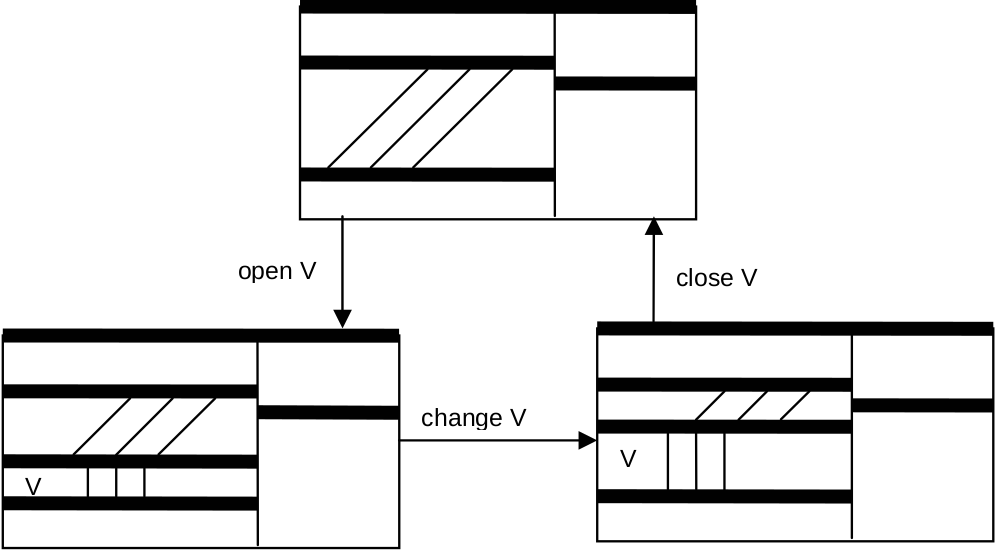
\includegraphics[width=.75\textwidth]{i/8}
  \caption{Basic operations on viewers}
  \label{fig:operation}
\end{figure}

The last group provides miscellaneous services.
\begin{itemize}
  \item \verb|This| identifies the viewer displayed at \verb|(X, Y)|.
  \item \verb|Next| returns the next upper neighbor of a given displayed viewer \verb|V|.
  \item \verb|Recall| allows recalling and restoring the most recently closed viewer.
  \item \verb|Locate| assists heuristic allocation of new viewers.
    For any given track and desired minimum height, it offers a choice
    of some distinguished viewers in this track:
    \begin{itemize}
      \item the \verb|fil|\textcolor{gray}{ler} viewer,
      \item the one at \verb|bot|\textcolor{gray}{tom},
      \item an \verb|alt|\textcolor{gray}{ernative} choice, and
      \item the viewer of \verb|max|\textcolor{gray}{imum} height.
    \end{itemize}
  \item Finally, \verb|Broadcast| broadcasts a message to the display area, that is,
    sends the given message to all currently displayed viewers.
\end{itemize}

It is now a good time to throw a glance behind the scenes.
Let us start with revealing \verb|Viewer| internal data structure.
Remember that according to the principle of information hiding
an internal data structure is fully private to the containing module
and accessible only through the module’s procedural interface.  Fig \ref{fig:snapshot}
shows a data structure view of the display snapshot taken in Fig \ref{fig:overlay}.
Note that the overlaid tracks and viewers are still part of the internal data structure.
\begin{figure}[h!]
  \centering
  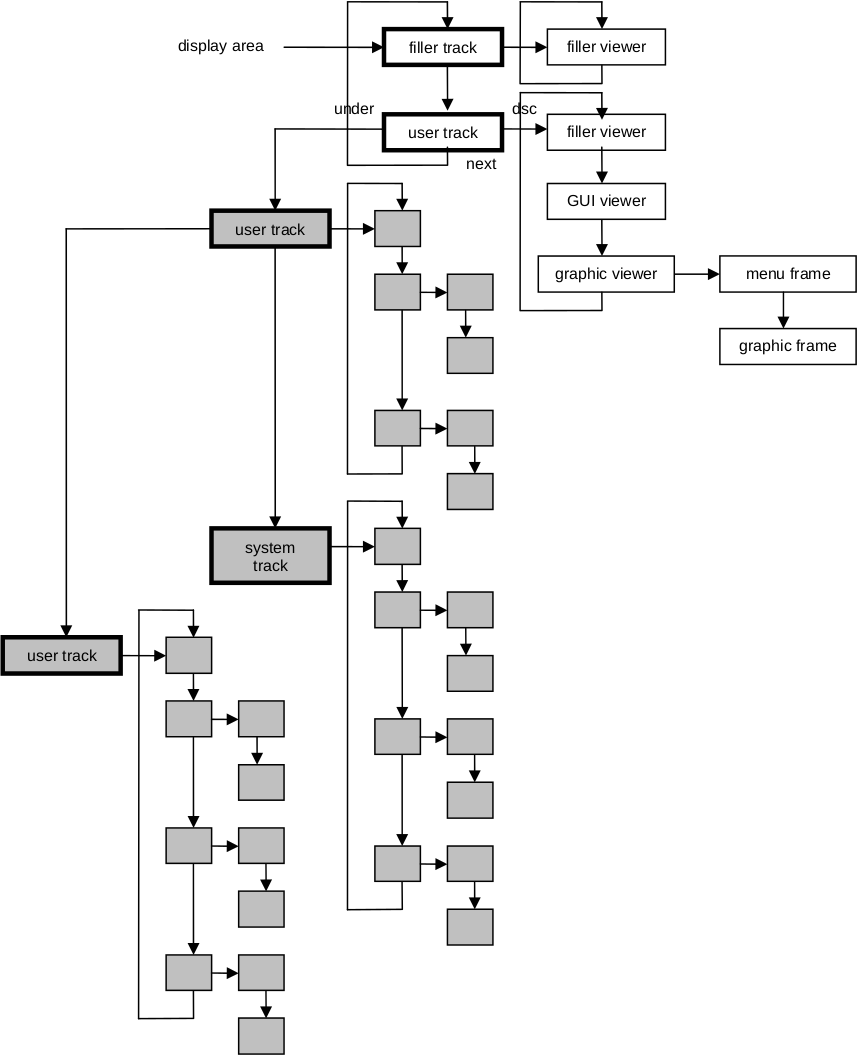
\includegraphics[width=\textwidth]{i/9}
  \caption{Internal data structure snapshot of Fig \ref{fig:overlay}}
  \label{fig:snapshot}
\end{figure}

In the data structure we recognize an anchor that represents the display area
and points to a list of tracks, each track pointing to a list of viewers,
each viewer in turn pointing to a list of arbitrary sub-frames.
Both the list of tracks and the list of viewers are closed to a ring,
where the filler track (filling up the display area)
and the filler viewers (filling up the tracks) act as anchors.
Additionally, each track points to a (possibly empty) list of tracks lying underneath.
These frames are invisible on the display, and shaded in Fig \ref{fig:snapshot}.

Technically, the track descriptor \verb|TrackDesc| is a private extension
of the viewer descriptor \verb|ViewerDesc|.
Repeating the declarations of viewer descriptors and frame descriptors,
we get to this hierarchy of types:
\begin{verbatim}
   TrackDesc = RECORD (ViewerDesc)
                      under: Display.Frame   END;

  ViewerDesc = RECORD (FrameDesc) state: INT END;

   FrameDesc = RECORD  next, dsc: Frame;
                      X, Y, W, H: INT;
                          handle: Handler    END;
\end{verbatim}

It is noteworthy that the data structure of the VM is heterogeneous with \verb|Frame| as base type.
It provides a nice example of a nested hierarchy of frames with the additional property
that the 1st 2 levels correspond to the 1st 2 levels in the type hierarchy defined by
\verb|Track|, \verb|Viewer|, and \verb|Frame|.

In an object-oriented environment objects are autonomous entities in principle.  However,
they may be bound to some higher instance (other than the system) temporarily.  For example,
we can look at the objects belonging to a module's private data structure as bound to this module.
Deciding if an object is currently bound then becomes a fundamental problem.  In the case of viewers,
this information is contained in an extra instance variable called \verb|state|.

As a system invariant, we have for every viewer $V$
\[ V\text{ is bound to module }Viewers \Leftrightarrow V.state \neq 0 \]
If we call any displayed viewer \emph{visible} and
each covered by an overlaying track \emph{suspended}, we can refine this invariant to
\begin{align*}
\{V\text{ is }&  visible\!\!\!\!\!\!\!\!\!\!\!\!\!\!\!\!\!\!\!\!\!\!\!\!\!\!\!&\Leftrightarrow V.state > 0\}&\text{ and }\\
\{V\text{ is }&suspended\!\!\!\!\!\!\!\!\!\!\!\!\!\!\!\!\!\!\!\!\!\!\!\!\!\!\!&\Leftrightarrow V.state < 0\}&
\end{align*}
In addition,
more detailed information about the kind of viewer $V$ is given by the magnitude $|V.state|$:
\begin{table}[h!]
  \centering
  \begin{tabular}{r l}
    $|V.state|$ & kind of viewer \\\hline
              0 & closed \\
              1 & filler \\
             -1 & productive
  \end{tabular}
\end{table}
\\The magnitude $|V.state|$ is kept invariant by \verb|Viewers|.
It could be used, for example, to distinguish different levels of importance or preference
with the aim of supporting a smarter algorithm for heuristic new viewers allocation.
$state$ is read-only to modules other than \verb|Viewers|.

We are now sufficiently prepared to understand how the exported \verb|Viewers| procedures
work behind.  They all operate on the internal dynamic data structure just explained.
\begin{itemize}
  \item \verb|This|, \verb|Next|, \verb|Locate|, \verb|Change| use it as a reference only
    or operate on individual elements
  \item \verb|InitTrack|, \verb|OpenTrack|, \verb|Open| add new elements, and
  \item \verb|CloseTrack|, \verb|Close| remove elements.
\end{itemize}
Most have side-effects on existing elements ($size$ or $state$).

Let us now change perspective and look at \verb|Viewers| as
a general low-level viewer manager (VMer) whose exact contents are unknown to it
(and whose controlling software might have been developed years later).
In short, let us look at \verb|Viewers| as a manager of black boxes.
Such an abstraction immediately makes it impossible for the implementation to call fixed procedures
for, say, changing a viewer's size or state.
The facility needed is a \emph{message-oriented interface}.
\begin{verbatim}
  TYPE ViewerMsg = RECORD (Display.FrameMsg) id,
                          X, Y, W, H, state: INT END;
\end{verbatim}

There're 3 variants of \verb|Viewer| messages, discriminated by \verb|id|:
\begin{table}[h!]
  \centering
  \begin{tabular}{l}
    restore contents, \\
    modify height (extend or reduce at bottom), and \\
    suspend (close temporarily or permanently).
  \end{tabular}
\end{table}
\\The additional components of the message inform about the desired new location, size, and state.
The following table lists senders, messages, and recipients of viewer messages.
\begin{table}[h!]
  \setlength{\tabcolsep}{1pt}
  \begin{tabular}{l|l|c r}
    \small{Originator} & \multicolumn{1}{c}{Message} & \multicolumn{2}{|c}{Recipients} \\\hline
    \small{OpenTrack}  & \small{suspend temporarily}
                       & \multicolumn{2}{l}{\small{viewers covered by opening track}} \\
    \small{CloseTrack} & \small{suspend permanently}
                       & \multicolumn{2}{l}{\small{viewers in closing track}}         \\
    \small{Open}       & \small{modify or suspend}
                       &        upper        &  opening viewer \\
    \small{Change}     & \small{modify}
                       & \small{neighbor of} & changing viewer \\
    \small{Close}      & \small{suspend permanently} & \multicolumn{2}{r}{closing viewer}
  \end{tabular}
\end{table}

\subsection{Menu Viewers}
\label{sub:menuviewers}
So far, we have treated viewers abstractly.
Next step we focus on a special class called \emph{menu viewers}.
From the earlier definition we know they're characterized by a structure
consisting of 2 vertically tiled \emph{descendant} frames,
\begin{table}[h!]
  \centering
  \begin{tabular}{r l}
    a frame of & at the \\\hline
    menu       & top, and \\
    contents   & bottom.
  \end{tabular}
\end{table}
\\Because the nature and contents of these frames are typically unknown
by their “ancestor” (or “parent”) viewer,
a collection of abstract messages is again a postulating form of interface.
As net effect, the handling of menu viewers boils down to a combination
of preprocessing, transforming and forwarding messages to the descendant frames.
In short, the display space is hierarchically organized and message passing within it
obeys the pattern of strict parental control.

Again, we start detailed discussion with module interface:
\begin{verbatim}
  DEFINITION MenuViewers;
    IMPORT Viewers, Display;        (*message ids*)
    CONST extend = 0; reduce = 1; move = 2;
    TYPE Viewer = POINTER TO ViewerDesc;
         ViewerDesc = RECORD (Viewers.ViewerDesc)
                             menuH: INT        END;
         ModifyMsg = RECORD (Display.FrameMsg)
                            id, dY, Y, H: INT  END;
  
    PROC Handle(       V: Display.Frame;
                   VAR M: Display.FrameMsg);

    PROC New(Menu , Main: Display.Frame;
             menuH, X, Y: INT             ): Viewer;
  END MenuViewers.
\end{verbatim}
The interface represented by this definition is conspicuously narrow.
There are just 2 procedures:
\begin{itemize}
  \item[a] generator procedure \verb|New|, and

    Returns a newly created menu viewer displaying the 2 (arbitrary) frames passed as parameters.

  \item[a] standard message handler \verb|Handle|.

    Implements the entire “behavior” of an object and in particular
    the above message dispatching functionality.
\end{itemize}

Message handlers in Oberon are implemented in the form of procedure variables that obviously
must be initialized properly at object creation time.  In other words, some concrete behavior
must explicitly be bound to each object, where different instances of the same object type
could potentially have a different behavior and/or the same instance could change its behavior
during its lifetime.  Our object model is therefore \emph{instance-centered}.

Conceptually, the creation of an object is an atomic action consisting of 3 basic steps:
\begin{enumerate}
  \item Allocate memory block;
  \item Install message handler;
  \item Initialize state variables.
\end{enumerate}
In the case of a standard menu \verb|V|\textcolor{gray}{iewer} creation:
\begin{verbatim}
  NEW(V); V.handle := Handle; V.dsc      := Menu;
          V.menuH  := menuH ; V.dsc.next := Main
\end{verbatim}
\verb|New| equals to \verb|create V; open V at X,Y|.
Opening \verb|V| needs \verb|Viewers|' assistance.

Implementing \verb|Handle| embodies the standard message handling strategy.
This is a coarse-grained view:
\begin{verbatim}
IF message reports about user interaction THEN
  IF variant is mouse tracking THEN
    IF mouse is in menu region THEN
      IF mouse is in upper menu region and
         left key is pressed THEN
        handle changing of viewer
      ELSE delegate handling to menu-frame
      END
    ELSE
      IF mouse is in main-frame THEN
        delegate handling to main-frame
      END
    END
  ELSIF variant is keyboard input THEN
    delegate handling to menu frame;
    delegate handling to main frame
  END

ELSIF message defines generic operation THEN
  IF message requests copy (clone) THEN
    send copy-message to menu frame to get a copy;
    send copy-message to main frame to get a copy;
    create menu viewer clone from copies
  ELSE
    delegate handling to menu frame;
    delegate handling to main frame
  END

ELSIF message reports about change of contents THEN
  delegate handling to menu frame;
  delegate handling to main frame

ELSIF message requests change of location/size THEN
  IF operation is restore THEN
    draw viewer area and border;
    send menu frm modify-msg to make extend from H 0;
    send main frm modify-msg to make extend from H 0
  ELSIF operation is modify THEN
    IF operation is extend THEN
      extend viewer area and border;
      send modify-msg to menu frm to make it extend;
      send modify-msg to main frm to make it extend
    ELSE (*reduce*)
      send modify-msg to main frm to make it reduce;
      send modify-msg to menu frm to make it reduce;
      reduce viewer area and border
    END
  ELSIF operation is suspend THEN
    send main frm modify-msg to make reduce to H 0;
    send menu frm modify-msg to make reduce to H 0
  END
END
\end{verbatim}

In principle, the handler acts as a message dispatcher that either processes a message directly
and/or delegates its processing to the descendant frames. Note that the handler's main alternative
statement discriminates precisely among the 4 basic categories of messages.

From the above outlined algorithm, handling copy messages, that is, requests for generating
a copy or clone of a menu viewer, we can derive a general recursive scheme for the creation
of a clone of an arbitrary frame:
\begin{enumerate}
  \item Send copy message to each element in the list of descendants;
  \item Generate copy of the original frame descriptor;
  \item Attach copies of descendants to the copy of descriptor.
\end{enumerate}

The essential point here is the use of new outgoing messages
in order to process a given incoming message.
We can regard message processing as a transformation
mapping incoming messages into a set of outgoing ones, with possible side-effects.
The simplest one, the input message being simply passed on to descendant(s),
is called \emph{delegation}.

As a fine point we clarify that the above algorithm is designed to create a deep copy
of a composite object (a menu viewer in our case).  If a shallow copy would be desired,
the descendants would not have to be copied, and the original descendants
instead of their copies would be attached to the copy of the composite object.

Another example of message handling is provided by mouse tracking.  Assume that
a mouse message is received by a menu viewer while the mouse is located in the upper part
of its menu frame and the left mouse key is kept down.  This means "change viewer's height
by moving its top line vertically".  No message to express the required transformation
of the sub-frames yet exists.  Consequently, module \verb|MenuViewer|s takes advantage of
our open (extensible) message model and simply introduces one called:
\begin{verbatim}
  ModifyMsg = RECORD (Display.FrameMsg)
                id, dY, Y, H: INT
              END;
\end{verbatim}
Field \verb|id| specifies one of the following 2 variants:
\begin{enumerate}
  \item \emph{extend}, or

    Requests the frame to move by the vertical translation vector \verb|dY|
    and then extend to height \verb|H| at bottom.

  \item \emph{reduce}.

    Requests the frame to reduce to height \verb|H| at bottom
    and then move by \verb|dY|.
\end{enumerate}
In both cases \verb|Y| indicates the Y-coordinate of the new lower-left corner.
Fig \ref{fig:modify} summarizes this graphically.
\begin{figure}[h!]
  \centering
  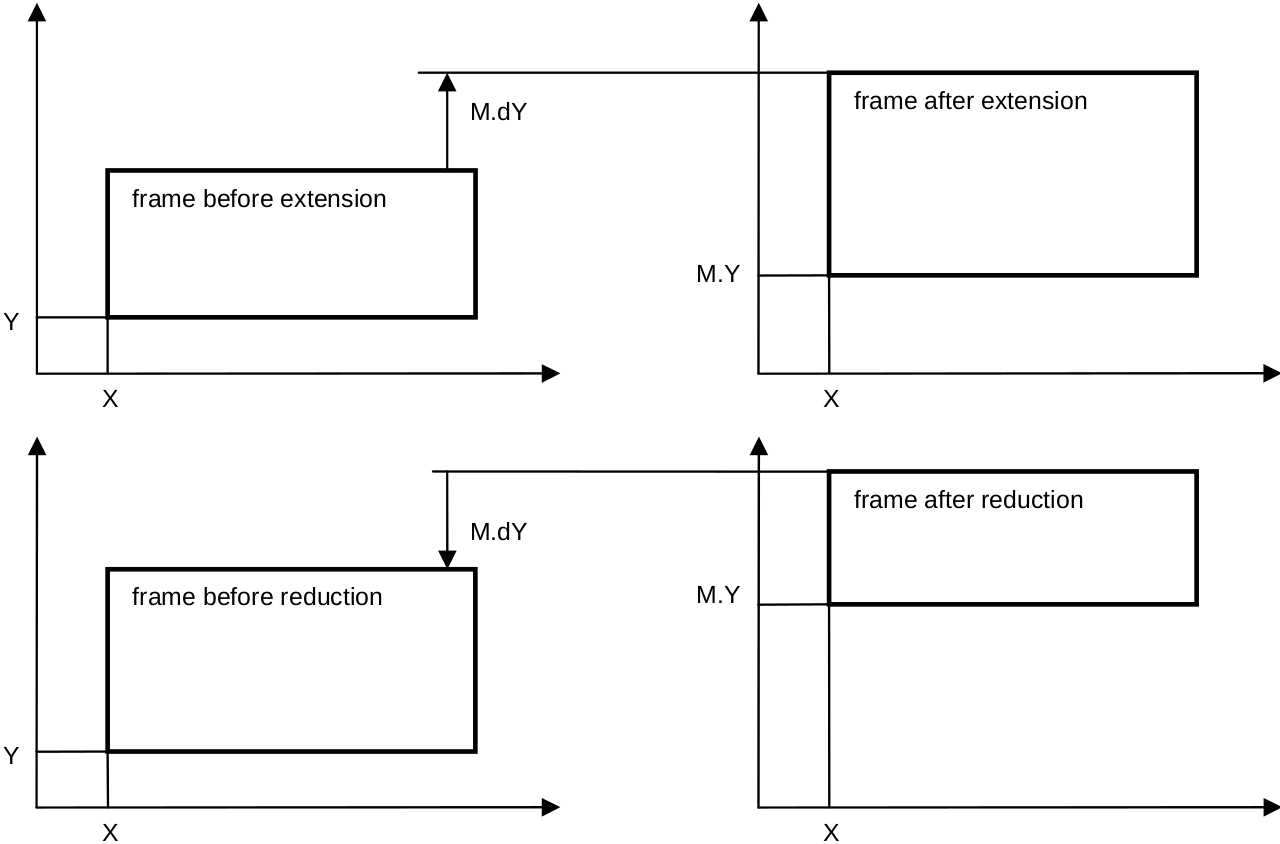
\includegraphics[width=.9\textwidth]{i/a}
  \caption{The modify frame operation}
  \label{fig:modify}
\end{figure}

Messages arriving from the VMer requesting the receiving viewer to extend or reduce
at its bottom are also mapped into \verb|ModifyMsg|s. Of course, no translation, $dY = 0$.

The attentive reader might perhaps have asked why the standard handler
is exported by \verb|MenuViewers| at all.  The thought behind is code reusability.
For example, a message handler for a subclass of menu viewers could be implemented effectively
by reusing menu viewer's standard one.  After having first handled all new or differing cases
it would simply (super-)call the standard handler subsequently.

\subsection{Cursor Management}
Traditionally, a cursor indicates and visualizes on the screen the current location of the caret
in a text or, more generally, the current \emph{focus of attention}.
A small arrow or similar graphic symbol is typically used for this purpose.
In Oberon, we have slightly generalized and abstracted this concept.
A cursor is a path in the logical display area whose current position can be made visible by a \emph{marker}.

The VMer and the cursor handler are 2 concurrent users of the same display area.
Actually, we should imagine 2 parallel planes,
\begin{table}[h!]
  \centering
  \begin{tabular}{r l}
              & displaying \\\hline
          one & viewers, and \\
    the other & cursors.
  \end{tabular}
\end{table}
\\If there's just 1 physical plane we take care of painting markers non-destructively, for example
in inverse-video mode.  Then, no precondition must be established before drawing a marker.
However, in the case of a viewer task painting destructively in its viewer's area,
the area must be locked first after turning invisible all markers in the area.

The technical support of cursor management is also contained in \verb|Oberon|.
The corresponding API:
\begin{verbatim}
DEFINITION Oberon;
  TYPE Marker = RECORD Fade,Draw: PROC(x,y: INT) END;
       Cursor = RECORD marker: Marker; X,Y: INT;
                                        on: BOOL END;
  VAR Arrow, Star   : Marker;
      Mouse, Pointer: Cursor;

  PROC OpenCursor(VAR c: Cursor);
  PROC FadeCursor(VAR c: Cursor);
  PROC DrawCursor(VAR c: Cursor;
                  VAR m: Marker; X, Y: INT);
  PROC MarkedViewer(): Viewers.Viewer;
  PROC RemoveMarks(X, Y, W, H: INT);
  ...
END Oberon.
\end{verbatim}
The state of a cursor is given by
\begin{table}[h!]
  \centering
  \begin{tabular}{r l}
    \verb|on|     & its mode of visibility, \\
    \verb|(X, Y)| & its position in the display area, and \\
    \verb|marker| & the current marker.
  \end{tabular}
\end{table}
\\\verb|Marker| is an abstract data type with an interface consisting of operations
  \verb|Fade| and
  \verb|Draw|.
The main benefit of this abstraction is once more conceptual independence
of the underlying hardware.  For example, they can
\begin{itemize}
  \item adapt to a given monitor hardware with built-in cursor support or,
    in case of absence of such support, simply
  \item be implemented as identical procedures (an involution)
    drawing the marker pattern in inverse video mode.
\end{itemize}

The functional interface to cursors consists of 3 operations:
\begin{table}[h!]
  \centering
  \begin{tabular}{l l}
    ~-\verb|Cursor| & to \\\hline
    \verb|Open| & open a new cursor, \\
    \verb|Fade| & switch off the marker of an open cursor, and \\
    \verb|Draw| & extend the path of a cursor to a new position \\
                & and mark it with the given marker.
  \end{tabular}
\end{table}
\\We emphasize that
the marker representing a given cursor can change its shape dynamically on the fly.

2 cursors are predefined:
\begin{table}[h!]
  \centering
  \begin{tabular}{r c l}
    cursor         & represents & \small{built-in }marker\small{ typically} \\\hline
    \verb|Mouse|   & the mouse  & \small{a small NW-pointing }\verb|Arrow| \\
    \verb|Pointer| &  a global  & \small{a }\verb|Star|\small{ symbol} \\
                   & \small{system pointer}
  \end{tabular}
\end{table}
\\The pointer can be used to mark any displayed object.
It serves primarily as an implicit parameter of commands.

2 assisting service procedures are added in connection with the predefined cursors:
\begin{table}[h!]
  \setlength{\tabcolsep}{3pt}
  \begin{tabular}{l|l}
    \verb|Marked| & \small{returns the viewer currently marked by the pointer,} \\
    \verb|-Viewer|& \small{equivalent to \verb|Viewers.This(Pointer.X, Pointer.Y)|.} \\\hline
    \verb|Remove| & \small{turns invisible within a given rectangle in display area,} \\
    \verb|-Marks| & \small{used to lock the rectangle for its caller.}
  \end{tabular}
\end{table}

Summary the essential concept points of cursor handling:
\begin{itemize}
  \item By virtue of the use of
    \begin{itemize}
      \item abstract markers, and
      \item the logical display area,
    \end{itemize}
    any potential hardware dependence is encapsulated in system modules
    and is therefore hidden from the application programmer.
    Cursors are moving uniformly within the whole display area,
    even across screen boundaries.

  \item Cursor handling is decentralized by delegating it to the individual handlers
    that are installed in viewers.  Typically, a handler reacts on the receipt
    of a mouse tracking message by drawing the mouse cursor at the indicated new position.
    The benefit of such individualized handling is flexibility.  For example,
    a smart local handler might choose the shape of the visualizing marker
    depending on the exact location, or it might force the cursor onto a grid point.

  \item Even though cursor handling is decentralized, there is some intrinsic support
    for cursor drawing built into the \verb|Cursor| declaration.
    Cursors are full value objects and, as such, can "memorize" their current state.
    Consequently, the interface operations \verb|FadeCursor| and \verb|DrawCursor|
    need to refer to the desired future state only.

  \item Looking at the VMer as one user of the display area, the cursor handler
    is the 2nd (and logically concurrent) user of the same resource.  If there is
    just one physical plane implementing the display area, any region must be locked
    by a current user before destructive painting.  Therefore,
    markers are usually painted non-destructively in inverse-video mode.
\end{itemize}

Let us now recapitulate the entire section.
\begin{itemize}
  \item The central resource managed by the display subsystem is the \emph{logical display area}
    whose purpose is abstraction from the underlying display monitor hardware.

    The display area is primarily used by the VMer for the accommodation of tracks and viewers,
    which are merely the 1st 2 levels of a potentially unlimited nested hierarchy of display frames.
    For example, standard menu viewers contain 2 subordinate frames:
    \begin{itemize}
      \item a menu frame, and
      \item a main frame of contents.
    \end{itemize}

  \item Viewers are treated as black boxes by the VMer and are addressed via messages.

    Viewers and, more generally frames, are used as elements of \emph{message-based interfaces}
    connecting the display subsystem with other subsystems like
    \begin{itemize}
      \item the task scheduler, and
      \item the various document managers.
    \end{itemize}

  \item Finally, the display area is also the living room of cursors.  In Oberon,
    a cursor is a marked path, 2 standard cursors \verb|Mouse| and \verb|Pointer| are predefined.
\end{itemize}

%\chapter{Statements and Expressions}
The specification of an action is called a statement. Statements can be interpreted (executed), and
that interpretation (execution) has an effect. The effect is a transformation of the state of the
computation, the state being represented by the collective values of the program's variables. The most
elementary action is the assignment of a value to a variable. The assignment statement has the form
\begin{verbatim}
  assignment = designator ":=" expression.
\end{verbatim}
and its corresponding action consists of 3 parts in this sequence:
\begin{enumerate}
  \item Evaluate the designator designating a variable.
  \item Evaluate the expression yielding a value.
  \item Replace the value of the variable identified in 1. by the value obtained in 2.
\end{enumerate}
Simple examples of assignments are:
\begin{verbatim}
  i := 1    x := y+z
\end{verbatim}
Here $i$ obtains the value 1, and $x$ the sum of $y$ and $z$, and the previous values are lost.
Evidently, every variable in an expression must previously have been assigned a value. Observe that
the following pairs of statements, executed in sequence, do not have the same effect:
\begin{verbatim}
  i := i+1; j := 2*i
  j := 2*i; i := i+1
\end{verbatim}
Assuming the initial value $i = 0$, the 1st pair yields $i = 1$, $j = 2$, whereas the 2nd pair yields
$j = 0$.  If we wish to exchange the values of variables $i$ and $j$, the statement sequence
\begin{verbatim}
  i := j; j := i
\end{verbatim}
will not have the desired effect. We must introduce a temporary value holder, say $k$, and specify
the 3 consecutive assignments
\begin{verbatim}
  k := i; i := j; j := k
\end{verbatim}
An expression is in general composed of several operands and operators. Its evaluation consists of
applying the operators to the operands in a prescribed sequence, in general taking the operators
from left to right. The operands may be constants, or variables, or functions. (The latter will be
explained in a later chapter.) The identification of a variable will, in general, again require the
evaluation of a designator. Here we shall confine our presentation to simple variables designated
by an identifier. Arithmetic expressions (there exist other expressions too) involve numbers,
numeric variables, and arithmetic operators. These include the basic operations of addition (+),
subtraction (-), multiplication (*), and division. They will be discussed in detail in the chapter on
basic data types. Here it may suffice to mention that the slash (/) is reserved for dividing real
numbers, and that for integers we use the operator DIV which truncates the quotient.

An expression consists of consecutive terms. The expression
\begin{verbatim}
  T0 + T1 + ... + Tn
\end{verbatim}
is equivalent to
\begin{verbatim}
  ((T0 + T1) + ...) + Tn
\end{verbatim}
and is syntactically defined by the rules
\begin{verbatim}
  SimpleExpression =[+|-] term {AddOperator term}.
  AddOperator = + | - | OR
\end{verbatim}

\textbf{Note}: for the time being, the reader may consider the syntactic entities expression and
SimpleExpression as equivalent. Their difference and the operators OR, AND, and NOT will be
explained in the chapter on the data type BOOL.

Each term similarly consists of factors. The term
\begin{verbatim}
  F0 * F1 * ... * Fn
\end{verbatim}
is equivalent to
\begin{verbatim}
  ((F0 * F1) * ... ) * Fn
\end{verbatim}
and is syntactically defined by the rules
\begin{verbatim}
  term = factor {MulOperator factor}.
  MulOperator = * | / | DIV | MOD | &.
\end{verbatim}
Each factor is either a constant, a variable, a function, or an expression itself enclosed by
parentheses.

Examples of (arithmetic) expressions are
\begin{verbatim}
  2*3 + 4*5       = (2*3)+(4*5)   = 26
  15 DIV 4 * 4    = (15 DIV 4)*4  = 12
  15 DIV (4*4)    = 15 DIV 16     = 0
  2 + 3*4 - 5     = 2 + (3*4) - 5 = 9
  6.25/1.25 + 1.5 = 5.0 + 1.5     = 6.5
\end{verbatim}
The syntax of factors, implying that a factor may itself be an expression, is evidently recursive. The
general form of designators will be explained later; here it suffices to know that an identifier
denoting a variable or a constant is a designator.
\begin{verbatim}
  factor = number | string | set | designator
    [ActualParameters] | (expression) | ~factor.
\end{verbatim}
The rules governing expressions are actually quite simple, and complicated expressions are rarely
used. Nevertheless, we must point out a few basic rules that are well worth remembering.
\begin{enumerate}
  \item Every variable in an expression must previously have been assigned a value.
  \item 2 operators must never be written side by side. For instance \verb|a * -b| is illegal and
    must be written as \verb|a*(-b)|.
  \item The multiplication sign must never be omitted when a multiplication is required. For
    example, \verb|2n| is illegal and must be written as \verb|2*n|.
  \item MulOperators are binding more strongly than AddOperators.
  \item When in doubt about evaluation rules (i.e. precedence of operators), use additional
    parentheses to clarify. For example, \verb|a+b*c| may just as well be written as
    \verb|a+(b*c)|.
\end{enumerate}
The assignment is but one of the possible forms of statements. Other forms will be introduced in the
following chapters. We enumerate these forms by the following syntactic definition
\begin{verbatim}
  statement = [ assignment | ProcedureCall | IfStatement
    | WhileStatement | RepeatStatement | ForStatement ].
\end{verbatim}
Several of these forms are structured statements, i.e. some of their components may be statements
again. Hence, the definition of statement is, like that of expressions, recursive.

The most basic structure is the sequence. A computation is a sequence of actions, where each
action is specified by a statement, and is executed after the preceding action is completed. This
strict sequentiality in time is an essential assumption of sequential programming. If a statement
$S_1$ follows $S_0$, then we indicate this sequentiality by a semicolon
\[  S_0; S_1 \]
This statement separator (not terminator) indicates that the action specified by $S_0$ is to be
followed immediately by the action corresponding to $S_1$. A sequence of statements is syntactically
defined as
\begin{verbatim}
  StatementSequence = statement {; statement}.
\end{verbatim}
The syntax of statements implies that a statement may consist of no symbols at all. In this case, the
statement is said to be empty and evidently denotes the null action. This curiosity among statements
has a definite reason: it allows semicolons to be inserted at places where they are actually
superfluous, such as at the end of a statement sequence.

%\chapter{Control Structures}
It is a prime characteristic of computers that individual actions can be selected, repeated, or
performed conditionally depending on some previously computed results. Hence the sequence of
actions performed is not always identical with the sequence of their corresponding statements. The
sequence of actions is determined by control structures indicating repetition, selection, or
conditional execution of given statements.

\section{Repetitive Statements}
The most common situation is the repetition of a statement or statement sequence under control of
a condition: the repetition continues as long as the condition is met. This is expressed by the 
\emph{while statement}. Its syntax is
\begin{verbatim}
  WhileStatement = WHILE expr DO StatementSequence END
\end{verbatim}
and its corresponding action is:
\begin{enumerate}
  \item Evaluate the condition which takes the form of an expression yielding
    the value \verb|TRUE| or \verb|FALSE|;
  \item If the value is \verb|TRUE|, execute the statement sequence and then repeat with step 1;
    if the value is \verb|FALSE|, terminate.
\end{enumerate}
The expression is of type \verb|BOOL|. This will be further discussed in the chapter on data types.
Here it suffices to know that a simple comparison is a Boolean expression. An example was given
in the introductory example, where repetition terminates when the 2 comparands have become
equal. Further examples involving while statements are:
\begin{enumerate}
  \item Initially, let $q = 0$ and $r = x$; then count the number of times $y$ can be subtracted
    from $x$, i.e. compute the quotient $q = x$\verb| DIV |$y$, and remainder $r = x$\verb| MOD |$y$,
    if $x$ and $y$ are natural numbers.
    \begin{verbatim}
      WHILE r >= y DO r := r-y; q := q+1 END
    \end{verbatim}
  \item Initially, let $z = 1$ and $i = k$; then multiply $z$ $k$ times by $x$, i.e. compute
    $z = xk$, if z and k are natural numbers:
    \begin{verbatim}
      WHILE i > 0 DO z := z*x; i := i-1 END
    \end{verbatim}
\end{enumerate}
When dealing with repetitions, it is important to remember the following points:
\begin{enumerate}
  \item During each repetition, progress must be made towards meeting the goal, namely "getting
    closer" to satisfying the termination condition. An obvious corollary is that the condition
    must be somehow affected from within the repeated computation. The following statements are
    either incorrect or dependent on some critical precondition as stated.
    \begin{verbatim}
      WHILE i > 0 DO
        k := 2*k (*i is not changed*)
      END
 
      WHILE i # 0 DO
        i := 1-2 (*i must be even and positive*)
      END
 
      WHILE n # i DO
        n := n*i; i := i+1
      END
    \end{verbatim}
  \item If the condition is not satisfied initially, the statement is vacuous, i.e. no action
    is performed.

  \item In order to obtain a grasp of the effect of the repetition, we need to establish a
    relationship that is stable, called an invariant. In the division example above, this is the
    equation $q*y + r = x$ holding each time the repetition is started. In the exponentiation
    example it is $z * x^i = x^k$ which, together with the termination condition $i = 0$ yields
    the desired result $z = x^k$.

  \item The repetition of identical computations should be avoided (although a computer has
    infinite patience and will not complain). A simple rule is to avoid expressions within
    repetitive statements, in which no variable changes its value. For example, the statement
    \begin{verbatim}
      WHILE i < 3*N DO tab[i] := x + y*z + z*i;
                       i := i+1 END
    \end{verbatim}
    should be formulated more effectively as
    \begin{verbatim}
      n := 3*N; u := x + y*z;
      WHILE i < n DO tab[i] := u + z*i; i := i+1 END
    \end{verbatim}
\end{enumerate}

In addition to the while statement, there is the \emph{repeat statement}, syntactically defined as
\begin{verbatim}
  RepeatStatement = REPEAT StatementSequence UNTIL expr
\end{verbatim}
The essential difference to the while statement is that the termination condition is checked each
time after (instead of before) execution of the statement sequence. As a result, the sequence is
executed at least once. An advantage is that the condition may involve variables that are undefined
when the repetition is started.
\begin{verbatim}
  REPEAT i := i+5; j := j+7; k := i DIV j UNTIL k > 23
  REPEAT r := r-y; q := q+1 UNTIL r < y
\end{verbatim}

\section{Conditional Statements}
The conditional statement, also called if statement, has the form
\begin{verbatim}
IfStatement = IF expr THEN StatementSequence
          {ELSIF expr THEN StatementSequence}
                     [ELSE StatementSequence]
              END
\end{verbatim}
The following example illustrates its general form.
\begin{verbatim}
     IF R1 THEN S1
  ELSIF R2 THEN S2
  ELSIF R3 THEN S3
           ELSE S4 END
\end{verbatim}
The meaning is obvious from the wording. However, it must be remembered that the expressions
\verb|R1 ... R3| are evaluated one after the other, and that as soon as one yields the value
\verb|TRUE|, its corresponding statement sequence is executed, whereafter the \verb|IF| statement
is considered as completed. No further conditions are tested. Examples are:
\begin{verbatim}
     IF x = 0 THEN s :=  0
  ELSIF x < 0 THEN s := -1
              ELSE s :=  1 END

  IF ODD(k) THEN z := z*x END
  IF k > 10 THEN k := k-10; d := 1
            ELSE d := 0 END
\end{verbatim}

The constructs discussed so far enable us to develop a few simple, complete programs as
subsequently described. The 1st example is an extension of our introductory example computing
the greatest common divisor $gcd$ of 2 natural numbers $x$ and $y$. The extension consists in
the addition of 2 variables $u$ and $v$, and statements which lead to the computation of the
least common multiple $lcm$ of $x$ and $y$. The $lcm$ and $gcd$ are related by the equation
\begin{verbatim}
  lcm(x,y) * gcd(x,y) = x*y
\end{verbatim}

As explained earlier, this and following examples will be formulated as command procedures and
are assumed to be embedded in module \verb|Pattern| defined in \ref{ch:1ex} which imports
modules \verb|Texts| and \verb|Oberon|.
\begin{verbatim}
  PROC gcdlcm*;
    VAR x, y, u, v: INT; S: Texts.Scanner;
  BEGIN Texts.OpenScanner(S, Oberon.Par.text,
                             Oberon.Par.pos):
    Texts.Scan(S); x := S.i;
    Texts.WriteString(W, " x =");
    Texts.WriteInt(W, x, 6);
    Texts.Scan(S); y := S.i;
    Texts.WriteString(W, " y =");
    Texts.WriteInt(W, y, 6);
    u := x; v := y;
    (*gcd(x,y) = gcd(x0,yO), x*v + y*u = 2*x0*y0*)
    WHILE x # y DO
      IF x > y THEN x := x-y; u := u+v
               ELSE y := y-x; v := v+u
      END
    END;
    Texts.WriteInt(W, x, 6);
    Texts.WriteInt(W, (u+v) DIV 2, 6);
    Texts.WriteLn(W);
    Texts.Append(Oberon.Log, W.buf)
  END gcdlcm.
\end{verbatim}
This example again shows the nesting of control structures. The repetition expressed by a while
statement includes a conditional structure expressed by an if statement, which in turn includes
2 statement sequences, each consisting of 2 assignments. This hierarchical structure is made
transparent by appropriate indentation of the "inner" parts.

Another example demonstrating a hierarchical structure computes the real number $x$ raised to
the power $i$, where $i$ is a non-negative integer.
\begin{verbatim}
  PROC Power*;
    VAR i: INT; x, z: REAL; S: Texts.Scanner;
  BEGIN Texts.OpenScanner(S, Oberon.Par.text,
                             Oberon.Par.pos);
    Texts.Scan(S);
    WHILE S.class = Texts.Real DO
      x := S.x; Texts.WriteString(W, " x =");
      Texts.WriteReal(W, x, 16); Texts.Scan(S);
      i := S.i; Texts.WriteString(W, " i =");
      Texts.WriteInt(W, i, 4);
      z= 1.0:
      (* z * x^i = x0^i0 *)
      WHILE i > 0 DO z := z*x; i := i-1 END;
      Texts.WriteReal(W, z, 16);
      Texts.WriteLn(W); Texts.Scan(S)
    END;
    Texts.Append(Oberon.Log, W.buf)
  END Power.
\end{verbatim}
Here we subject the computation to yet another repetition: Each time a result has been computed,
another value pair $x, i$ is requested. This outermost repetition is controlled by the relation
\verb|S.class = Texts.Real|, which indicates whether a real number $x$ had actually been read.
As an example, activation of the command
\begin{verbatim}
  M.Power 5.0 2   2.0 5   3.0 3 ~
\end{verbatim}
will generate the results \verb|25.0, 32.0, 27.0|.

The straight-forward computation of a power by repeated multiplication is, although obviously
correct, not the most economical. We now present a more sophisticated and more efficient solution.
It is based on the following consideration: The goal of the repetition is to reach the value $i = 0$.
This is done by successively reducing $i$, while maintaining the invariant $z * x^i = x_0^{i_0}$,
where $x_0$ and $i_0$ denote the initial values of $x$ and $i$. A faster algorithm therefore must
rely on decreasing $i$ in larger steps. The solution given here halves $i$. But this is only possible,
if $i$ is even. Hence, if $i$ is odd, it is 1st decremented by 1. Of course, each change of $i$ must
be accompanied by a corrective action on $z$ in order to maintain the invariant.
\begin{itemize}
  \item A detail: the subtraction of 1 from $i$ is not expressed by an explicit statement, because
    it is performed implicitly by the subsequent division by 2.
  \item 2 further details are noteworthy:
  \begin{enumerate}
    \item The function \verb|ODD(i)| is \verb|TRUE|, if $i$ is an odd number, \verb|FALSE| otherwise.
    \item $x$ and $z$ denote real values, as opposed to integer values. Hence, they can represent
      fractions, too.
  \end{enumerate}
\end{itemize}
\begin{verbatim}
  PROC Power*;
    VAR i: INT; x, z: REAL; S: Texts.Scanner;
  BEGIN Texts.OpenScanner(S, Oberon.Par.text,
                             Oberon.Par.pos);
    Texts.Scan(S);
    WHILE S.class = Texts.Real DO
      x := S.x; Texts.WriteString(W, " x =");
      Texts.WriteReal(W, x, 16): Texts.Scan(S);
      i := S.i; Texts.WriteString(W, " i=");
      Texts.WriteInt(W, i, 4);
      z := 1.0;
      WHILE i > 0 DO
        (* z* x^i = x0^i0 *)
        IF ODD(i) THEN z := z*x END;
        x := x*x; i := i DIV 2
      END;
      Texts.WriteReal(W, z, 16);
      Texts.WriteLn(VW); Texts.Scan(S)
    END;
    Texts.Append(Oberon.Log, W.buf)
  END Power.
\end{verbatim}

The next sample command has a structure that is almost identical to the preceding program. It
computes the logarithm of a real number $x$ whose value lies between 1 and 2. The invariant in
conjunction with the termination condition ($b=0$) implies the desired result $sum=\log_2{x}$.
\begin{verbatim}
  PROC Log2*;
    VAR x, a, b, sum: REAL; S: Texts.Scanner;
  BEGIN Texts.OpenScanner(S, Oberon.Par.text,
                             Oberon.Par.pos);
    Texts.Scan(S);
    WHILE S.class = Texts.Real DO
      x := S.x; Texts.WriteReal(W, x, 15); (*1<=x<2*)
      a :=x; b := 1.0; sum := 0.0;
      REPEAT (*log_2(x) = sum + b*log_2(a)*)
        a := a*a; b := 0.5*b;
        IF a >= 2.0 THEN
          sum := sum + b; a := 0.5*a
        END
      UNTIL b < 1.0E-7;
      Texts.WriteReal(W, sum, 16);
      Texts.WriteLn(W); Texts.Scan(S)
    END;
    Texts.Append(Oberon.Log, W.buf)
  END Log2.
\end{verbatim}

Normally, routines for computing standard mathematical functions need not be programmed in
detail, because they are available from a collection of modules similar to those for input
and output. Such a collection is, somewhat inappropriately, called a library. In the following
example, again exhibiting the use of a repetitive statement, we use routines for computing the
cosine and the exponential function from a library called Math and generate a table of values
for a damped oscillation. Typically, the available standard routines include the $sin$, $cos$,
$exp$, $ln$ (logarithm), $sqrt$ (square root), and the $arctan$ functions.
\begin{verbatim}
  PROC Oscillation*;
    CONST dx = 0.19634953; (*pi/16*)
    VAR i, n: INT; x, y, REAL; S: Texts.Scanner;
  BEGIN Texts.OpenScanner(S, Oberon.Par.text,
                             Oberon.Par.pos):
    Texts.Scan(S); n := S.i; Texts.WriteInt(W, n, 6);
    Texts.Scan(S); r := S.x; Texts.WriteReal(W, r, 15);
    Texts.WriteLn(W); i := 0; x := 0.0;
    REPEAT x := x + dx; i := i+1;
           y := Math.exp(-r*x) * Math.cos(x);
           Texts.WriteReal(W, x, 15);
	   Texts.WriteReal(W, y, 15);
	   Texts.WriteLn(W)
    UNTIL i >= n;
    Texts.Append(Oberon.Log, W.buf)
  END Oscillation.
\end{verbatim}

%\section{1964: Family Notion and 8-bit Byte}
IBM's System 360 was announced in 1964. It brought 2 other innovations. The
1st was the notion of a computer family. Up to this time, every computer had its
own structure and performance; it was sort of unique. Now System 360 consisted
of many incarnations of one and the same instruction set. Each incarnation, called
model, had its distinct performance figures, size and price. But all of them looked
the same to the programmer. In this sense they formed a family; they featured the
same architecture. This is where the word architecture in connection with
computers appeared.

It goes without saying that the different models had very different implementations
of the hardware, although they were handling the same software. For the first time,
the technique of emulation was used extensively. The smaller models used the
novel technique of micro-programs. The genuine hardware always interpreted the
same program, namely an interpreter of the 360 instruction set. The interpreter
was defined in so-called microcode. This micro-code rested in a small but very fast
microcode memory, typically a read-only memory implemented in a proprietary
technology. The consequence was that some of the 360's instructions were fast,
others slow in comparison. It was possible to include some very complex and hard
to understand instructions. Some of them even included loops in the micro-code.

The 2nd novelty was that the smallest individually addressable unit in memory
was not the word, but the byte, and that this byte consisted of 8 bits. So far, that
unit was considered as consisting of 6 bits, and the word length of all computers
were multiples of 6. An immediate negative consequence had been the limitation of
character sets (ASCII and IBM's EBCDIC) to 64 characters. The extension to 256
characters was a welcome benefit.

This revolutionary step also dispensed with "variable length data computers", such
as the ubiquitous IBM 1401, which featured string instructions, which operated on
sequences of 9-bit bytes, the 9th bit acting as a string termination indicator.

%\chapter{Storage Layout and Management}
\label{ch:MM}
Centralized RM (CRM) is a crucial property of Oberon.
\begin{description}
  \item[Its advantage] is that replication of management algorithms and a premature partitioning
    of resources are avoided.
  \item[The disadvantage] is that management algorithms are fixed once and forever and remain
    the same for all applications.
\end{description}
The success of a CRM therefore depends crucially on its flexibility and its efficient implementation.
This chapter presents the scheme and the algorithms governing main storage in Oberon.

\section{Layout and run-time organization}
The storage layout of Oberon is determined by the structure of code and data typical in the
use of modular, high-level PLs, and in particular of the language Oberon.
It suggests the subdivision of storage into 3 areas:
\begin{description}
  \item[module space] Each module specifies procedures (code) and global (static) variables.
    Its initialization can be regarded as a procedure implicitly called upon loading. Space
    must be allocated for code and data in \emph{blocks} by the loader. Typically, modules
    contain very few global variables, hence the space size is primarily determined by code.
  \item[workspace (stack)] Execution of every command invokes a sequence of procedures, each
    of which uses (possibly zero) parameters and local variables. Since procedure calls and
    completions follow a strict first-in last-out order, the stack is the uniquely suited
    strategy for local storage allocation. Deallocation upon completion of a procedure is
    achieved by merely resetting the pointer identifying the top of the stack. Since this
    operation is performed by a single instruction, it costs virtually no time. Because
    Oberon is a single-process system, a single stack suffices. Furthermore, after completion
    of a command, the stack is empty. This fact will be important in simplifying the scheme
    for reclamation of dynamically allocated space.
  \item[dynamic space (heap)] Apart from global (static) variables, and local (stack-allocated)
    variables, a program may refer to anonymous variables referenced through pointers. Such
    variables are allocated truly dynamically through calls of an explicit \verb|NEW| operation.
    These variables are allocated in the so-called \emph{heap}. Their deallocation is "automatic",
    when free storage is needed and they are no longer referenced from any of the loaded modules.
    This process is called \emph{garbage collection} (GC). Every record allocated in the heap
    contains a (hidden) pointer to the type descriptor, called \emph{type tag}, used by GC.
\end{description}
Unfortunately, the number of distinct spaces is larger than 2. If it were 2, no arbitrary
size limitation would be necessary; merely the sum of their sizes would be inherently limited
by the size of the store. In the case of 3 spaces, arbitrarily determined size limits are
unavoidable. Address mapping hardware can alleviate (and delegate) this problem using a
virtual address space which is so large that limits will hardly ever be reached.

Such a scheme is implemented by tables mapping virtual into physical addresses, requiring
multiple memory accesses for every reference. Of course, the need for a double or a triple
access for every memory reference is avoided by a translation cache in the (hardware) unit.
Nevertheless, a decrease in performance is unavoidable for each cache miss. Furthermore,
an additional subcycle is required for every access in order to look up the cached translation
table. Without a virtual address scheme, each module block must consist of an integral number
of physically adjacent pages. Holes generated by the release of modules must be reused. We
employ the simple scheme of marking the released space as a hole, and of allocating a new
block in the 1st hole encountered that is large enough (1st-fit strategy). Considering the
relative infrequency of module releases, efforts to improve the strategy are not worth the
resulting added complexity.

It is remarkable that the code for module allocation and release without virtual addressing
is only marginally more complicated than with it. The only remaining advantages of an MMU are a
better storage utilization, because no holes occur (a negligible advantage), and that inadvertent
references to unloaded modules, e.g. via installed procedures, lead to an invalid address trap.

It is worth recalling that the concept of address mapping was introduced as a requirement for
virtual memory implemented with disks as backing store, where pages could be moved into the
background in order to obtain space for newly required pages, and could then be retrieved from
disk on demand, i.e. when access was requested. This scheme is called \emph{demand paging}.
It is not used in Oberon, and one may fairly state that demand paging has lost its significance
with the availability of large, primary stores.

Experience in the use of the RISC predecessor Ceres leads to the conclusion that whereas
address translation through an MMU was an essential feature for multi-user OSes, it constitutes
a dispensible overkill for single-user workstations. The fact that modern semiconductor technology
made it possible to integrate the entire translation and caching scheme into a single chip,
or even into the processor itself, led to the hiding (and ignoring) of the scheme's considerable
complexity. Its side effects on execution speed are essentially unpredictable. This makes systems
with MMU virtually unusable for applications with tight real-time constraints. The RISC processor
does indeed not feature an address mapping unit.
\begin{figure}[h!]
  \label{fig:storage-layout}
  \centering
  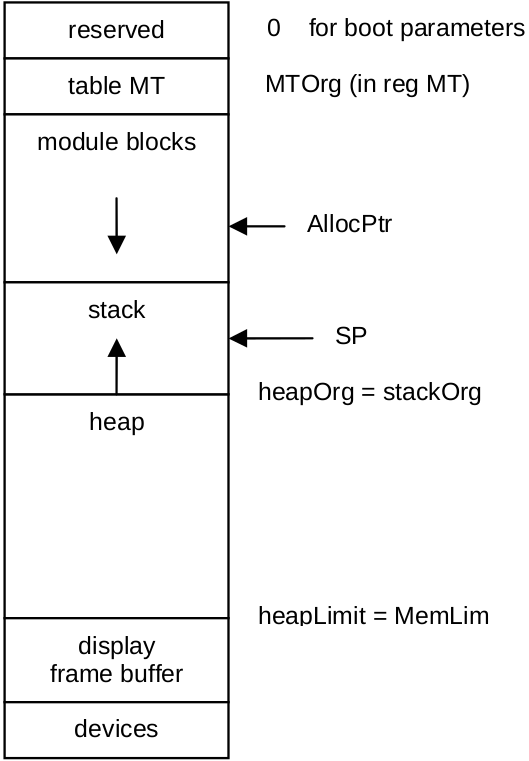
\includegraphics[width=.6\textwidth]{i/q}
  \caption{Storage layout}
\end{figure}

The RISC processor features 16 registers (of 32 bits). R0 - R11 are for expression evaluation.
R12 - R15 have fixed, system-wide usage:
\begin{table}[h!]
  \centering
  \begin{tabular}{l l}
    R12 & address of the module table MT (typically constant) \\
    R13 & base address for variables in the current module SB \\
        & (static base) \\
    R14 & stack pointer SP \\
    R15 & return address LNK (fixed by RISC's BL instruction)
  \end{tabular}
\end{table}

The used memory layout is shown in Figure \ref{fig:storage-layout}.

\section{Heap Management}
The term \emph{dynamic storage} is used here for all variables that are allocated neither
statically (global variables) nor on the stack (local variables), but through invocation
of the intrinsic procedure \verb|NEW| in the heap. Such variables are anonymous and are
referenced exclusively via pointers.

The space allocated to such dynamic variables becomes free and reusable as soon as the last
reference to it vanishes. This event is hard, and in multiprocess systems even impossible
to detect. The usual remedy is to ignore it and instead to determine the accessibility of
all allocated variables (records, objects) only at the time when more storage space is needed.
This process is then called \emph{garbage collection}.

Oberon does not provide an explicit deallocation procedure allowing the programmer to signal
that a variable will no longer be referenced. The 1st reason for this omission is that
usually a programmer would not know when to call for deallocation. And 2ndly, this "hint"
could not be taken as trustworthy. An erroneous deallocation, i.e. one occurring when there
still exist references to the object in question, could lead to a multiple allocation of
the same space with disastrous consequences. Hence, it appears wise to fully rely on system
management to determine which areas of the store are truly reusable.

Before discussing the scheme for storage reclamation, which is the primary subject of
heap management, we turn our attention to the problem of allocation, i.e. the implementation
of procedure \verb|NEW|. The simplest solution is to maintain a list of free blocks and to
pick the 1st one large enough. This strategy leads to a relatively large fragmentation of
space and produces many small elements, particularly in the 1st part of the list. We
therefore employ a somewhat more refined scheme and maintain 4 lists of available space.
3 of them contain pieces of fixed size, namely 32, 64, and 128 bytes. The 4th list contains
pieces whose size is any multiple of 256. We note that the choice of the values permits the
merging of any 2 contiguous elements into an element of the next list. This scheme keeps
fragmentation, i.e. the emergence of small pieces in large numbers, reasonably low with
minimal effort. The body of procedure \verb|NEW| consists of relatively few instructions,
and typically only a small fraction of them needs to be executed.

The statement \verb|NEW(p)| is compiled into an instruction sequence assigning the address
of pointer variable $p$ to a fixed register (\verb|R0|) and the type tag to another register
(\verb|R1|). The type tag is a pointer to a type descriptor containing information required
by GC. This includes the size of the space occupied and now to be allocated. The effect of
\verb|NEW| is the assignment of the address of the allocated block to $p$, and the assignment
of the tag to a prefix of the block. (see Fig. \ref{fig:allocation})
\begin{figure}[h!]
  \label{fig:allocation}
  \centering
  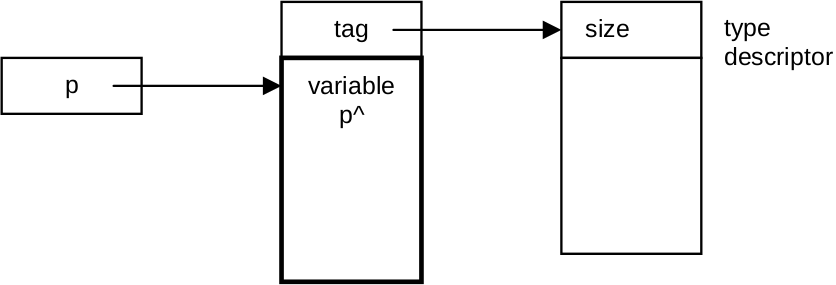
\includegraphics[width=\textwidth]{i/r}
  \caption{Heap allocation of dynamic variable $p$\^{} by NEW($p$)}
\end{figure}

In conclusion, we emphasize that this scheme makes the allocation of an object very efficient.
Nevertheless, it is considerably more costly than that of a variable explicitly declared
and therefore allocated either globally or on the stack. We now turn to the problem of
storage reclamation or GC. There exist 2 essentially different schemes:
\begin{itemize}
  \item[$1^{st}$,] the reference counting, and
  \item[$2^{nd}$,] the mark-scan schemes.
\end{itemize}
In the former, every object carries a (hidden) \emph{reference count}, indicating the number
of existing references to it. The scheme works as follows:
\begin{enumerate}
  \item \verb|NEW(p)| initializes the reference count of $p$\^{} to 1.
  \item An assignment \verb|q := p| decrements the reference count of $q$\^{} by 1, performs
    the assignment, then increments the reference count of $p$\^{} by 1.
\end{enumerate}
When a reference count reaches zero, the element is linked into the free list. There are 2
disadvantages inherent in this approach:
\begin{enumerate}
  \item the non-negligible overhead in pointer assignments.
  \item circular data structures never become recognized as free,
    even if no external references point to their elements.
\end{enumerate}

Oberon employs the 2nd scheme which involves no hidden operations like the 1st one, but
relies on a process initiated when free storage has become scarce and more is needed.
It consists of 2 phases:
\begin{description}
  \item[mark phase] all referenced and therefore still accessible elements are marked.
  \item[scan phase] their unmarked complement is released.
\end{description}
Its primary disadvantage is that the process may be started at moments unpredictable to the
system's user. During the process, the computer then appears to be blocked. It follows that
an interactive system using mark-scan GC must guarantee that the process is sufficiently
fast in order to be hardly noticeable. Modern processors make this possible, even with
large main stores. Nevertheless, finding all accessible nodes in an entire computer system
within, say, a second appears to be a formidable feat.

We recognize that the mark phase essentially is a tree traversal, or rather a forest traversal.
The roots of the trees are all named pointer variables in existence. We shall postpone the
question of how these roots are to be found, and 1st present a quick tutorial about tree
traversal. In general, nodes of the traversed structure may contain many pointers (branches).
We shall, however, 1st restrict our attention to a binary tree, because the essential problem
and its solution can be explained better in this way.

The essential problem alluded to is that of storage utilization by the traversal algorithm itself.
Typically, information about the nodes already visited must be retained, be it explicitly, or
implicitly as in the case of use of recursion. Such a strategy is plainly unacceptable,
because the amount of storage needed is unpredictable and may become very large, and because
GC is typically initiated just when more storage is unavailable. The task may seem impossible,
yet a solution lies in the idea of inverting pointers along the path traversed, thus keeping
the return path open. It is embodied in the following procedure, whose task is to traverse
the tree given by the parameter root, and to mark every node. Mark values are assumed to
be initially 0. Let the data structure be defined by the types
\begin{verbatim}
  Ptr = POINTER TO Node;
  Node = RECORD m: INT; L, R: Ptr END;
\end{verbatim}
and the algorithm by the procedure
\begin{verbatim}
  PROC traverse(root: Ptr);
    VAR p, q, r: Ptr;
  BEGIN p := root; q := root;
    REPEAT (*p # NIL*) INC(p.m); (*mark*)
      IF p.L # NIL THEN (*pointer rotation*)
        r := p.L; p.L := p.R; p.R := q; q := p; p := r
      ELSE
        p.L := p.R; p.R := q; q := NIL
      END
    UNTIL p = q
  END traverse
\end{verbatim}
\begin{figure}[h!]
  \centering
  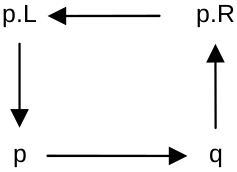
\includegraphics[width=.25\textwidth]{i/s}
  \label{fig:rotation}
  \caption{Rotation of four pointers}
\end{figure}
We note that only 3 local variables are required, independent of the size of the tree to be
traversed. The 3rd, $r$, is in fact merely an auxiliary variable to perform the rotation of
values $p.L$, $p.R$, $q$, and $p$ as shown in Fig. \ref{fig:rotation}. A snapshot of a tree
traversal is shown in Fig. \ref{fig:tree-traversal}.
\begin{figure}[h!]
  \centering
  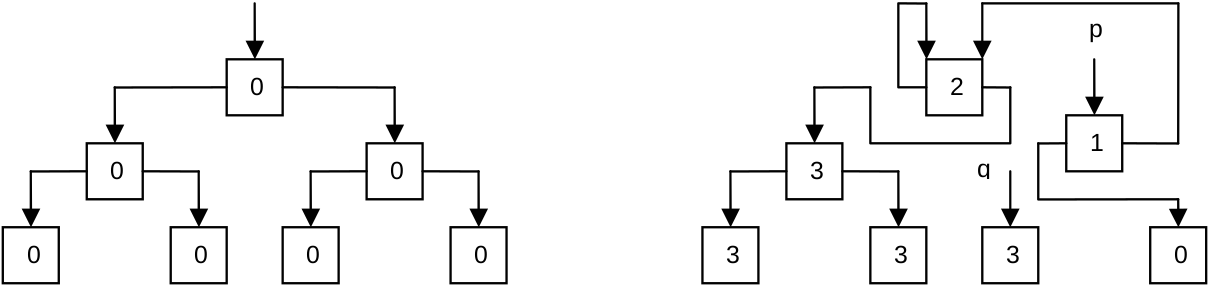
\includegraphics[width=\textwidth]{i/t}
  \label{fig:tree-traversal}
  \caption{Tree traversal (original at left, snapshot at right)}
\end{figure}

The pair $p$, $q$ of pointers marks the position of the process. The algorithm traverses
the tree in a left to right, depth 1st fashion. When it returns to the root, all nodes
have been marked. How are these claims convincingly supported? The best way is by analyzing
the algorithm at an arbitrary node. We start with the hypothesis H that, given the initial
state P, the algorithm will reach state Q, (see Fig \ref{fig:transition}). State Q differs
from P by the node and its descendants B and C having been marked, and by an exchange of p
and q. We now apply the algorithm to state P, assuming that B and C are not empty. The process
is illustrated in Fig \ref{fig:transition}. P0 stands for P in Fig. \ref{fig:tree-traversal}.
\begin{figure}[h!]
  \centering
  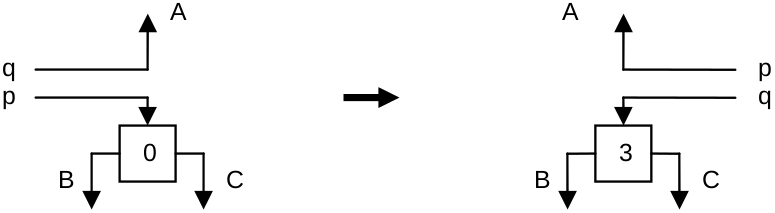
\includegraphics[width=\textwidth]{i/u}
  \label{fig:transition}
  \caption{Transition from state P to Q}
\end{figure}
Transitions $P0 \rightarrow P1$, $P2 \rightarrow P3$, and $P4 \rightarrow P5$ are the direct
results of applying the pointer rotation as specified by the sequence of five assignments
in the algorithm. Transitions $P1 \rightarrow P2$ and $P3 \rightarrow P4$ follow from the
hypothesis H being applied to the states P1 and P3: subtrees are marked and p, q interchanged.
We note in passing that the node is visited 3 times. Progress is recorded by the mark value
which is incremented from 0 to 3.

Fig. \ref{fig:transition-3-times}. demonstrates that, if H holds for steps $P1 \rightarrow P2$
and $P3 \rightarrow P4$, then it also holds for step $P1 \rightarrow P5$, which visits the
subtree p. Hence, it also holds for the step root $\rightarrow$ root, which traverses the entire tree.
\begin{figure}[h!]
  \label{fig:transition-3-times}
  \centering
  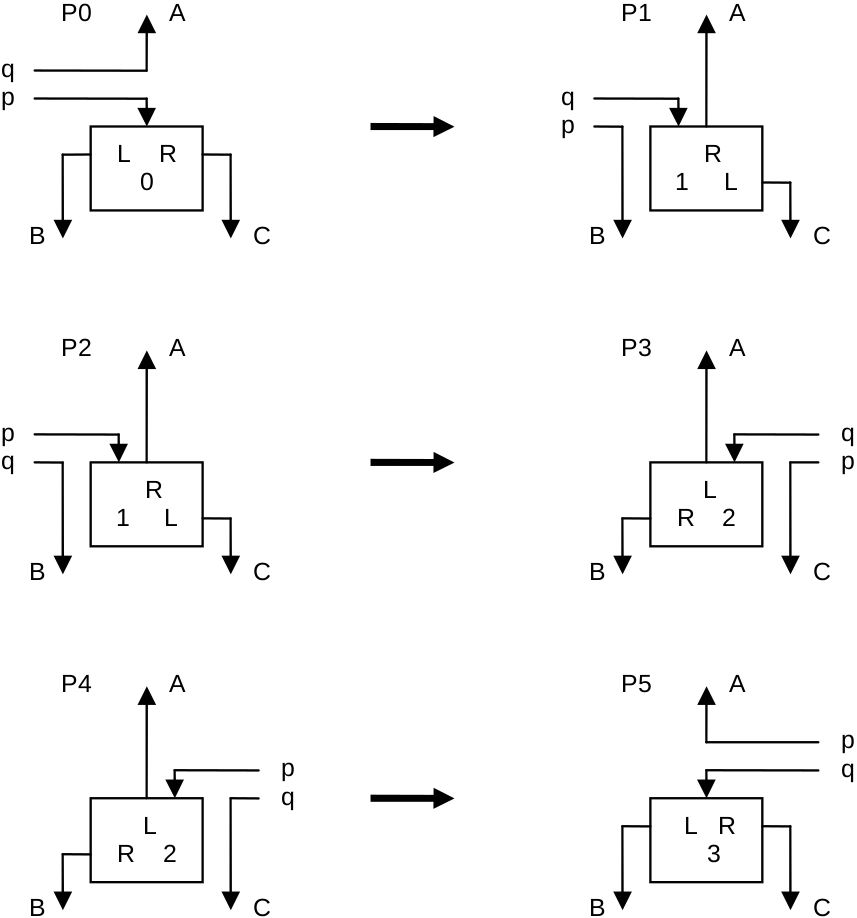
\includegraphics[width=.9\textwidth]{i/v}
  \caption{Transitions from P0 to P5, visiting nodes 3 times}
\end{figure}

This proof by recursion relies on the algorithm performing correct transitions also in the
case of p.L being NIL, i.e. B being the empty tree. In this case, state P1 is skipped; the
1st transition is $P0 \rightarrow P2$ (see Fig \ref{fig:transition-direct}).
If p.L is again NIL, i.e. also C is empty, the next transition is $P2 \rightarrow P4$.
This concludes the demonstration of the algorithm's correctness.
\begin{figure}[h!]
  \label{fig:transition-direct}
  \centering
  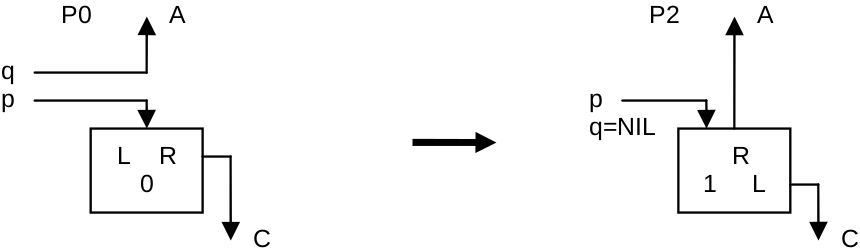
\includegraphics[width=\textwidth]{i/w}
  \caption{Direct transition from P0 to P2, if $p.L = NIL$}
\end{figure}

We now modify the algorithm of tree traversal to the case where the structure is not confined
to a binary tree, but may be a tree of any degree, i.e. each node may have any number $n$ of
descendants. For practical purposes, however, we restrict $n$ to be in the range $0 \leq n
\leq N$, and therefore may represent all nodes by the type
\begin{verbatim}
  Node = RECORD m, n: INT;
           dsc: ARRAY N OF Node
         END
\end{verbatim}
In principle, the binary tree traversal algorithm might be adopted almost without change,
merely extending the rotation of pointers from p.L, p.R, q, p to p.dsc[0], ... , p.dsc[n-1], q, p. However, this
would be an unnecessarily inefficient solution. The following is a more effective variant. Moreover, it
caters for the case of inhomogeneous graphs, where different nodes have different numbers of
descendants. The key lies in associating with every node, in addition to the tag, a 2nd private
field mk. It serves 2 purposes. The 1st is as a mark, with mk > 0 indicating that the node had
been visited. The 2nd is to store the address of the next descendant to be visited. The
underlying data structure is shown in Fig \ref{fig:record}. Type descriptors consist of the following fields:
\begin{table}[h!]
  \centering
  \setlength{\tabcolsep}{2pt}
  \begin{tabular}{l l}
    size & {\small in bytes, of the described record type,} \\
    base & {\small a table of pointers to the base types descriptors(3 elements only)} \\
    {\small offsets} & {\small of the descendant pointers in the described type(1 word each)}
  \end{tabular}
\end{table}
\begin{figure}[h!]
  \label{fig:record}
  \centering
  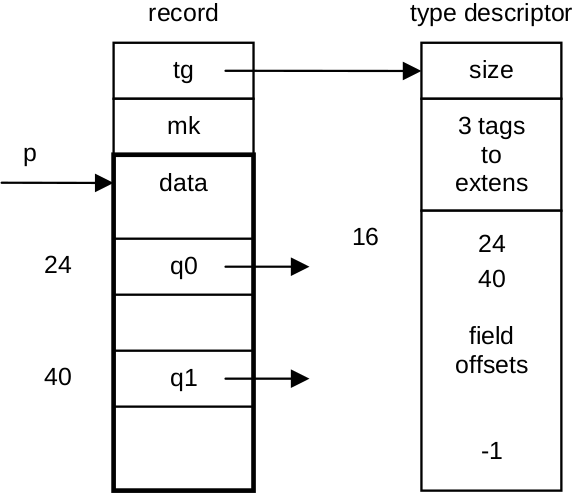
\includegraphics[width=.9\textwidth]{i/x}
  \caption{Record and its type descriptor}
\end{figure}

We note that the mark value, starting with zero (unmarked), is used as a counter of descendants
already traversed, and hence as an index to the descendant field to be processed next. The
algorithm can be applied not only to trees, but to arbitrary structures, including circular ones, if the
continuation condition p \# 0 (actually p >= heapOrg) is extended to (p >= heapOrg) \& (offadr = 0).
This causes a descendant that is already marked to be skipped. Here the array M stands for the
entire memory.
\begin{verbatim}
  PROC traverse(root: Ptr);
    VAR offadr, offset: INT; p, q, r: Ptr;
  BEGIN p := root; q := root;
    REPEAT (*p # NIL*) offadr := p.mk; (*mark*)
      IF offadr = 0 THEN
        tag := p.tg; offadr := tag + 16
      ELSE INC(offadr, 4) END;
      p.mk := offadr; offset := M[offadr];
      IF offset # -1 THEN (*move down*)
        r := M[p+offset]; offadr := M[r-4];
        IF offadr = 0 THEN
          M[p+offset] := q; q := p; p := r
        END
      ELSE (*move up*)
        offadr := M[q-4]; offset := M[offadr]
        IF p # q THEN
          r := M[q+offset]; M[q+offset] := p;
          p := q; q := r
        END
      END
    UNTIL (p = q) & (offset = -1)
  END traverse.
\end{verbatim}

The mark is included in each record's hidden prefix. The prefix takes 2 words only; the first is used
for the tag. The other is reserved for the garbage collector and used as mark and offset address.
The end of the list of descendant pointers is marked by an entry with value -1. And finally,
assignments involving M are expressed as
\begin{table}[h!]
  \centering
  \begin{tabular}{c|l}
    assignment & for \\\hline
    \verb|SYSTEM.GET(a, x)| & $x := M[a]$ \\
    \verb|SYSTEM.PUT(a, x)| & $M[a] := x$ \\
  \end{tabular}
\end{table}

The scan phase is performed by a relatively straight-forward algorithm. The heap, i.e. the storage
area between HeapOrg and HeapLimit (the latter is a variable), is scanned element by element,
starting at HeapOrg. Elements marked are unmarked, and unmarked elements are freed by linking
them into the appropriate list of available space.
As the heap may always contain free elements, the scan phase must be able to recognize them in
order to skip them or merge them with an adjacent free element. For this purpose, the free
elements are also considered as prefixed. The prefix serves to determine the element's size and to
recognize it as free due to a special (negative) mark value. The encountered mark values and the
action to be taken are:
\begin{table}[h!]
  \centering
  \begin{tabular}{c r c}
    $mk$ value &  state & action \\\hline
    $=0$     & unmarked & collect, mark free \\
    $>0$     &   marked & unmark \\
    $<0$     &     free & skip or merge
  \end{tabular}
\end{table}

\section{Kernel}
\label{sec:kernel}
The kernel lies at the bottom of the module hierarchy. It contains the procedures for
dynamic storage allocation and retrieval as described before. The procedures are \verb|New|,
\verb|Mark|, and \verb|Scan|. \verb|Kernel| also contains the driver routines for the disk.
They are used by modules \verb|FileDir| and \verb|Files|. The "disk" is actually an SD-card,
a high-volume flash-RAM. It is accessed purely sequentially, byte-wise, by a standard,
serial peripheral interface (SPI). Within \verb|Kernel| a table called \verb|SectorMap| is
allocated keeping track of blocks (sectors) occupied by files. A single bit indicates,
whether a sector is allocated or not. This table is accessed by the procedures
\verb|AllocSector|, \verb|MarkSector|, and \verb|FreeSector|. Reading and writing is done
sector-wise by procedures \verb|GetSector| and \verb|PutSector|. Sector numbers are always
a multiple of 29 for the purpose of redundancy checks.

Furthermore, the kernel contains a timer counting milliseconds and, perhaps, a real time
clock, showing date and time. Clock data are packed into a single word as follows:
\begin{figure}[h!]
  \label{fig:datetime}
  \centering
  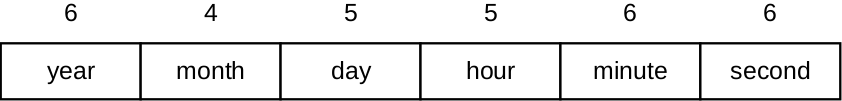
\includegraphics[width=\textwidth]{i/y}
  \caption{Encoding of date and time (year starting with 2000)}
\end{figure}
\begin{verbatim}
  DEFINITION Kernel;(*NW/PR 11.4.86/27.12.95/15.5.2013*)
    CONST SectorLength = 1024;
    TYPE Sector = ARRAY SectorLength OF BYTE;
    VAR allocated, NofSectors, heapOrg, heapLim,
        stackOrg, MemSize: INT;
    PROC New(VAR ptr: INT; tag: INT);
    PROC Mark(pref: INT);
    PROC Scan;
    PROC ResetDisk;
    PROC MarkSector(sec: INT);
    PROC FreeSector(sec: INT);
    PROC AllocSector(hint: INT; VAR sec: INT);
    PROC GetSector(src: INT; VAR dest: Sector);
    PROC PutSector(dest: INT; VAR src: Sector);
    PROC Time(): INT; (*milliseconds*)
    PROC Clock(): INT;
    PROC SetClock(dt: INT);
    PROC Install(adr, procadr: INT);
    PROC Init;
  END Kernel.
\end{verbatim}

\section{The storage management toolbox}
The user can obtain information about the system state and resources through its toolbox,
a set of commands contained in the too module \verb|System|. These commands are:
\begin{verbatim}
  PROC Watch;
  PROC Collect;  / n
  PROC SetClock; / year,month,day,hour,minute,second
\end{verbatim}
Command \verb|Watch| shows the amount of storage occupied in the heap, the number of disk
sectors allocated on the disk, and the number of tasks installed. The command \verb|Collect|
allows to control the frequency of GC. The number $n$ indicates how many commands are
executed before the next GC.

%\chapter{Device Driver(DD)}
\label{ch:DD}
\section{Overview}
Device drivers are collections of procedures that constitute the immediate interface between
hardware and software. They refer to those parts of the computer hardware that are usually called
peripheral. Computers typically contain a system bus which transmits data among its different parts.
Processor and memory are considered as its internal parts; the remaining parts, such as disk,
keyboard, display, etc, are considered as external or peripheral, notwithstanding the fact that they
are often contained in the same cabinet or board.

Such peripheral devices are connected to the system bus via special registers (data buffers) and
transceivers (switches, buffers in the sense of digital electronics). These registers and transceivers
are addressed by the processor in the same way as memory locations - they are said to be
memory-mapped - and they constitute the hardware interface between processor bus and device.
References to them are typically confined to specific driver procedures which constitute the
software interface.

Drivers are inherently hardware specific, and the justification of their existence is precisely that they
encapsulate these specifics and present to their clients an appropriate abstraction of the device.
Evidently, this abstraction must still reflect the essential characteristics of the device, but not the
details (such as e.g. the addresses of its interface registers).

Our justification to present the drivers connecting the Oberon with the RISC computer in
detail is on the one hand the desire for completeness. But on the other hand it is also in recognition
of the fact that their design represents an essential part of the engineering task in building a
system. This part may look trivial from a conceptual point of view; it certainly is not so in practice.
In order to reduce the number of interface types, standards have been established. The RISC
computer also uses such interface standards, and we will concentrate on them in the following
presentations. The following devices are presented:

\begin{enumerate}
	\item The Keyboard is considered as a serial device delivering one byte of input data per key stroke. It
is connected by a serial line according to the PS/2 and ASCII (American Standard Code for
Information Interchange) standards. The software is contained in module Input (Sect. 9.2), and the
hardware is explained in Sect. 17.2.1.
	\item The Mouse is a pointing device delivering coordinates in addition to key states. The software is
also part of module Input (Sect. 9.2).
	\item Display. The interface to the display is an area of memory that contains the displayed
information, exactly one bit per pixel for a monochrome display. This area is called frame buffer or
bitmap Here the size is of the display area is 768 lines and 1024 dots per line, representing a
raster. The software is module Display, which primarily consists of operations to draw frequently
occurring patterns. These operations are called raster-ops. They are explained in Section 4.5. The
actual display requires a hardware interface called a display controller. The connection between the
controller and the display follows the VGA-Standard (see Sect. 17.2.4).
	\item Disk. Our RISC computer does not use a magnetic, rotating disk for storing non-volatile data.
Instead, it uses an SD-card (flash-RAM). The driver is contained in module Kernel (Section 8.3).
The hardware is discussed in Sect. 17.2.2.
	\item Net. In the original text, a network was presented consisting of a bus connecting many
computers, based on the RS-485 standard. It was implemented by the serial communications
controller Zilog 8530, operating at a frequency of 230 Kb/s. The name SCC has been retained as a
generic interface, behind which the packet transport has now been re-implemented as a simple
wireless
network
(Nordic
nRF24L01
controller)
in
the
regulation-free
2.4GHz
industrial/scientific/medical (ISM) frequency band.
\end{enumerate}

In all driver modules the implementation-dependent procedures SYSTEM.PUT, SYSTEM.GET, and
SYSTEM.BIT are used to access the registers of the device interface. Their first parameter is the
address of the register, the second an expression or variable.

\section{Keyboard and mouse}
The driver procedures for the keyboard and the mouse are located in module Input. Available()
signals that a character has been typed on the keyboard, if its value is greater than 0. The
character is read by calling Read(ch). Module Input is restricting the data to the ASCII character set
Latin-1, i.e. the values lie in the range 0X <= ch < 80X (7-bit values). Mouse(k, x, y) yields the
current state of the mouse keys and the mouse's coordinates.
\begin{verbatim}
MODULE Input;
PROC Available(): INT;
PROC Read(VAR ch: CHAR);
PROC Mouse(VAR keys: SET; VAR x, y: INT);
PROC SetMouseLimits(w, h: INT);
PROC Init;
END Input.
\end{verbatim}

The driver software accesses the keyboard via the Standard PS/2 interface represented by an 8-bit
register for the received data kbdCode, and a single-bit flag indicating whether a byte had been
received.

The keyboard codes received from the keyboard via a PS/2 line are not identical with the character
values delivered to the Read procedure. A conversion is necessary. This is so, because modern
keyboards treat all keys in the same way, including the ones for upper case, control, alternative,
etc. Separate codes are sent to signal the pushing down and the release of a key, followed by
another code identifying which key had been pressed or released. This requires, besides a
translation table from codes to characters, a set of state variables. They are the global, Boolean
variables Recd, Up, Shift, Ctrl, and Ext. Procedure Peek determines whether an actual character is
present, or merely a code signalling a key shift. Peek controls the state.

Procedure Mouse fetches a word from the mouse interface register and decomposes it into its
components (key state and coordinates). (kb is the bit indicating whether a code had been received
from the keyboard).
\begin{figure}
	\label{fig:format}
	\centering
	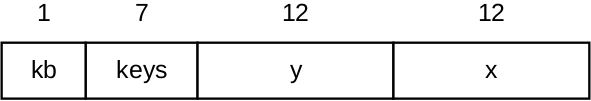
\includegraphics[width=.75\textwidth]{i/z}
	\caption{Format of the mouse register}
\end{figure}

\section{The SD-card (disk)}
SD-card are high-volume memory devices based on flash-store technology. They are typically
organized as individually accessible blocks of 1K bytes. The driver for the SD-card is contained in
module Kernel, which also handles allocation and reservation of blocks, here in analogy to rotating
disks still called sectors.
\begin{verbatim}
TYPE Sector = ARRAY SectorLength OF BYTE;
PROC GetSector(src: INT; VAR dst: Sector);
PROC PutSector(dst: INT; VAR src: Sector);
PROC AllocSector(hint: INT; VAR sec: INT);
PROC MarkSector(sec: INT);
PROC FreeSector(sec: INT);
\end{verbatim}

Data transfer is sequebtial and handled by procedures ReadSD and WriteSD by issuing
commands. These are for transmitting a block address, for receiving, and for sending a block of
data. Synchronous transmission of sequences of words follows the SPI standard, which uses 3
lines, one for data input, one for dats output, and one for the clock (see also Section 17.2.2). The
hardware interface contains a 32-bit register. The bit-rate is 8.3 MB/s.

\section{Serial asynchronous interface (RS 232)}
The RS-232 standard serves to transmit sequences of bytes over a data line asynchronously. This
implies that there is no separate clock line (see also Section 17.2.3). The hardware interface
contains a 10-bit register for the transmitter and one for the receiver. The data rate used here is
19200 bit/s. A byte is sent and received over the line by the following programs.
\begin{verbatim}
CONST data = -56; stat = -52; (*device register addresses*)
PROC Send(x: BYTE);
BEGIN
REPEAT UNTIL SYSTEM.BIT(stat, 1);
SYSTEM.PUT(data, x)
END Send;
PROC Rec(VAR x: BYTE);
BEGIN
REPEAT UNTIL SYSTEM.BIT(stat, 0);
SYSTEM.GET(data, x)
END Rec;
\end{verbatim}

These procedures are used in the driver module RS232 presented in Section 15.2. This module
itself is not used in the Oberon core, but it was instrumental in building the System on a host
computer and downloading it. It is characterized by a very simple interface.

\section{Serial communications controller (SCC)}
The interface of the driver for the network was taken over from the original design using a serial
communocations controller Zilog 8530. The implementation changed totally. It was designed by
Paul Reed for the wireless controller Nordic nRF24L01.
\begin{verbatim}
DEFINITION SCC;
TYPE Header =
RECORD valid: BOOL; dadr, sadr, typ: BYTE;
len: INT; (*of data following header*)
END ;
PROC Start(filter: BOOL);
PROC Send(VAR head: Header; buf: ARRAY OF BYTE);
PROC Available(): INT;
PROC ReceiveHead(VAR head: Header);
PROC Receive(VAR x: BYTE);
PROC Skip(m: INT);
PROC Stop;
END SCC.
\end{verbatim}

%\part{Apps}
%\section{1975: Micro Computers}
Microcomputers mentioned in the preceding paragraph were the visible result of
the immense progress made in semiconductor technology, in particular of the
efforts on miniaturization. Discrete transistors had been replaced by integrated
circuits containing themselves many transistors, all produced in the same
manufacturing step in a silicon foundry. Fairchild was leading the way, followed by
Intel, National Semiconductor, Motorola, and others. First, there was the (short-
lived) RTL technology (Resistor-Transistor Logic), soon to be super ceded by TTL
technology (Transistor-Transistor Logic). Packages of ICs successfully became
standardized founding the era of TTL chips, the series 74xxx. (Only the military
had their own, more expensive cookies, the 54xxx series). Also, a single supply
voltage of 5V belonged to the standard (only at the beginning augmented by -5V
and 12V for memory chips). This was definitely one of the most successful
standardization efforts in industrial history.

The building blocks of circuits were no longer transistors and resistors (and
occasionally a capacitor), but elementary circuits, such as gates, multiplexers,
decoders, adders, register arrays, and buffers. The heart of these micro computers
was a single chip of a novel dimension of complexity, a complete, small computer,
incorporating a simple arithmetic/logical unit, a set of data registers, an instruction
register and a program counter, that is, a complete control unit.

The (not quite) first microprocessor chips featured a data path of only 8 bits. The
prominent samples were the Intel 8080, the Motorola 6800, and the Rockwell
6502. Memory chips became available, first with 1K bits, then followed soon by 4K,
16K and even 64K (1980). As a result of this development it became relatively
easy to design and build small computers for modest amounts of money. Upgrades
of microprocessors followed soon, in particular the Motorola 6809 with a 16-bit
internal ALU.

A special line of microcomputers appeared soon thereafter (1975). They were
complete computer systems on a single chip, and they became known as micro-
controllers, to be used mostly in embedded systems. They consisted of a simple
ALU, a control unit, and a small amount of static memory (SRAM). They also
contained on-chip (programmable) program memory. In early versions, this
memory was writable only once (PROM), later versions contained erasable
memory (EPROM). The most successful ones came from Intel (8048, 8051) and
they were soon manufactured by the millions, driving down the cost to the order of
a dollar and entering cars, refridgerators, and television sets.

%\section{References}
  \begin{enumerate}
    \item \href{
      http://Awww.digilentinc.com/Data/Products/S3BOARD/S3BOARD_RM.pdf
    }{Xilinx, Spartan-3 Starter kit board user guide}

    \item \href{
      htto://www.inf.ethz.ch/personal/wirth/CompilerConstruction/index.html
    }{N. Wirth. Compiler Construction. Addison-Wesley, 1995.}
  \end{enumerate}

%\chapter{Parameters}
Procedures may be given parameters. They are the essential feature that make procedures so
useful. Consider again the previous example of procedure Add. Very likely a program contains
several arrays to which the procedure should be applicable. Redefining it for each such array would
be cumbersome, inelegant, and can be avoided by introducing its operand as a parameter as
follows.
\begin{verbatim}
  PROC Add(VAR x: Vector);
    VAR i: INT;
  BEGIN sum := 0:
    FOR i := 0 TO N-1 DO sum := x[i] + sum END
  END Add
\end{verbatim}
The parameter $x$ is introduced in the parameter list in the procedure heading. It thereby
automatically becomes a local object, in fact is a place-holder for the actual array that is
specified in the procedure calls
\begin{verbatim}
  Add(a); ... ; Add(b)
\end{verbatim}
The arrays $a$ and $b$ are called actual parameters which are substituted for $x$, which is called
formal parameter. The formal parameter's specification must contain its type. This enables a compiler
to check whether or not an appropriate actual parameter is supplied. We say that $a$ and $b$, the
actual parameters, must be compatible with the formal parameter $x$. In the example above, its type
is Vector, presumably declared in the environment of Add as
\begin{verbatim}
  TYPE Vector = ARRAY N OF REAL;
  VAR a, b: Vector
\end{verbatim}
A better version of Add would include not only the array, but also the result sum as a parameter.
We shall later return to this example. But first we need explain that there exist 2 kinds of formal
parameters, namely variable and value parameters. The former are characterized by the symbol
VAR, the latter by its absence.

We conclude this chapter by giving the syntax of procedure declarations and procedure calls:
\begin{verbatim}
  proc = prop | func
  prop = PROC id [params]; decls [BEGIN ss] END id
  func = PROC id [params]: type; decls [BEGIN ss]
                              [RETURN expr] END id
  params = ([param{; param}])
  param  = [VAR] ident{, ident}: {ARRAY OF} type
\end{verbatim}
Apart from the declaration of modules, we now have also encountered all forms of declarations.
\begin{verbatim}
  decls = [CONST {const;}] [TYPE {typdef;}]
          [VAR {field;}] {proc;}
\end{verbatim}

\section{Variable Parameters}
As its name indicates, the actual parameter corresponding to a formal variable parameter (specified
by the symbol VAR) must be a variable. The formal identifier then stands for that variable.
\begin{verbatim}
  PROC exchange(VAR x, y: INT);
    VAR z: INT;
  BEGIN z := x; x := y; y := z
  END exchange
\end{verbatim}
The procedure calls
\begin{verbatim}
  exchange(a, b); exchange(A[i], A[i+1])
\end{verbatim}
then have the effect of the above 3 assignments, each with appropriate substitutions made
upon the call. The following points should be remembered:
\begin{enumerate}
  \item Variable parameters may serve to transmit a computed result outside the procedure.
  \item The formal parameter acts as a place-holder for the substituted actual parameter.
  \item The actual parameter cannot be an expression, and therefore not a constant either,
    even if no assignment to its formal correspondent is made.
  \item If the actual parameter involves indices, these are evaluated when the formal-actual
    substitution is made.
  \item The types of corresponding formal and actual parameters must be the same.
\end{enumerate}

\section{Value Parameters}
Value parameters serve to pass a value from the calling side into the procedure and constitute the
predominant case of parameters. The corresponding actual parameter is an expression, of which a
variable or a constant are a particular and simple case. The formal value parameter must be
considered as a local variable of the indicated type. Upon call, the actual expression is evaluated
and the result is assigned to that local variable. As a consequence, the formal parameter may later
be assigned new values without affecting any part of the expression. In a sense, actual expression
and formal parameter become decoupled as soon as the procedure is entered. As an illustration,
we formulate the previously shown program to compute the power $z = x^i$ as a procedure. Note:
Assignments to value parameters are prohibited, if they are structured.
\begin{verbatim}
  PROC ComputePower(VAR z: REAL; x: REAL; i: INT);
  BEGIN z := 1.0:
    WHILE i > 0 DO
      IF ODD(i) THEN z := z*x END;
      x := x*x; i := i DIV 2
    END
  END ComputePower
\end{verbatim}
Possible calls are, for example
\begin{table}[h!]
  \centering
  \begin{tabular}{c|rll}
    procedure call & \multicolumn{3}{c}{for} \\\hline
    \verb|ComputePower(u   ,  2.5, 3)| &   $u$&:=&$2.5^3$ \\
    \verb|ComputePower(A[i], B[i], 2)| & $A_i$&:=&$B_i^2$ \\
  \end{tabular}
\end{table}

\textbf{Note}:
\begin{enumerate}
  \item If a formal parameter is an array or a record and not specified as a variable parameter,
    then assignments to elements are prohibited.
  \item In the example above $z$ and $x$ must be declared in distinct \verb|param|, because
    "\verb|VAR z, x: REAL|" would classify $x$ as a variable parameter too, making it impossible
    to place a general expression in its corresponding actual parameter place.
\end{enumerate}

\section{Open Array Parameters}
lf a formal parameter type denotes an array structure, its corresponding actual parameter
must be an array of the identical type. This implies that it must have elements of identical
type and the same bounds of the index range. Often this restriction is rather severe, and
more flexibility is highly desirable. It is provided by the facility of the so-called
\emph{open array} which requires that the types of the elements of the formal and actual
arrays be the same, but leaves the index range of the formal array open. In this case,
arrays of any size may be substituted as actual parameters. An open array is specified by
the element type preceded by \verb|ARRAY OF|. For example, a procedure declared as
\begin{verbatim}
  PROC P(s: ARRAY OF CHAR)
\end{verbatim}
allows calls with character arrays of arbitrary length. The actual length (number of
elements) is obtained by calling the standard function \verb|LEN(s)|.

%\chapter{Function Procedures}
So far we have encountered 2 possibilities to pass a result from a procedure body to its calling
place: the result is either assigned to a non-local variable or to a variable parameter. There
exists a 3rd method: the function procedure. It permits the use of the computed result (as an
intermediate value) in an expression. The function procedure identifier stands for a computation
as well as for the computed result. The procedure declaration is characterized by the indication
of the type of the result following the parameter list. As an example, we rephrase the power
computation given above.
\begin{verbatim}
  PROC power(x: REAL; i: INT): REAL;
    VAR z: REAL;
  BEGIN z := 1.0:
    WHILE i > 0 DO
      IF ODD(i) THEN z := z*x END;
      x := x*x; i := 1 DIV 2
    END;
    RETURN z
  END power
\end{verbatim}
Possible calls are
\begin{verbatim}
  u    := power(2.5, 3)
  A[i] := power(B[i], 2)
  u    := x + power(y, i+1) / power(z, i-1)
\end{verbatim}
The result of the function evaluation is specified as an expression following the symbol
\verb|RETURN| and immediately preceding the symbpl \verb|END|.

Calls inside an expression are called \emph{function designators}. Their syntax is the same
as that of procedure calls. However, a parameter list is mandatory, although it may be empty.
\begin{verbatim}
  ReturnStatement = "RETURN" [expression].
\end{verbatim}
We now revisit the previous example of adding the elements of an array and formulate it as
a function procedure:
\begin{verbatim}
  PROC sum(VAR a: Vector; n: INT): REAL;
    VAR i: INT; s: REAL;
  BEGIN s := 0.0:
    FOR i := 0 TO n-1 DO s := a[i]+s END;
    RETURN s
  END sum
\end{verbatim}
This procedure, as previously specified, sums the elements $a[0] \dots a[n-1]$, where $n$
is given as a value parameter, and may be different from (but not larger than!) the number
of elements $N$. A more elegant solution specifies $a$ as an open array, omitting the
explicit indication of the array's size.
\begin{verbatim}
  PROC sum(VAR x: ARRAY OF REAL): REAL;
    VAR i: INT; s: REAL;
  BEGIN s := 0.0:
    FOR i := 0 TOLEN(x)-1 DO's := x{i] +s END;
    RETURN s
  END sum
\end{verbatim}
Obviously, procedures are capable of generating more than one result by making assignments
to several variables. Only one value, however, can be returned as the result of a function.
This value, moreover, cannot be of a structured type. Therefore, the other results must be
passed to the caller via VAR parameter or assignment to variables that are not local to the
function procedure. Consider for example the following procedure which computes a primary
result denoted as the function's value and a secondary result used to count the number of
times the procedure is called.
\begin{verbatim}
  PROC square(x: INT): INT;
  BEGIN INC(n); RETURN x*x
  END square
\end{verbatim}
There is nothing remarkable about this example as long as the secondary result is used for
its indicated purpose. However, it might be misused as follows:
\begin{verbatim}
  m := square(m) +n
\end{verbatim}
Here the secondary result occurs as an argument of the expression containing the function
designator itself. The consequence is that e.g. the values \verb|square(m)+n| and
\verb|n+square(m)| differ, seemingly defying the basic law of commutativity of addition.

Assignments of values from within function procedures to non-local variables are called
\emph{side-effects}. The programmer should be fully aware of their capability of producing
unexpected results when the function is used inappropriately. We summarize:
\begin{enumerate}
  \item A function procedure specifies a result which is used at its place of call as an
    argument of an expression.
  \item The result of a function procedure cannot be structured.
  \item If a function procedure generates secondary results, it is said to have side-effects.
    These must be used with care. It is advisable to use a regular procedure instead,
    which passes its results via \verb|VAR| parameters.
  \item We recommend to choose function identifiers which are nouns rather than verbs. The
    noun then denotes the function's result. Boolean functions are appropriately labelled
    by an adjective.  In contrast, regular procedures should be designated by a verb
    describing their action.
\end{enumerate}

%\chapter{Recursion}
Procedures may not only be called, but can call procedures themselves. Since any procedure
that is visible can be called, a procedure may call itself. This self-reactivation is
called \emph{recursion}.  Its use is appropriate when an algorithm is recursively defined
and in particular when applied to a recursively defined data structure.

Consider as an example the task of listing all possible permutations of $n$ distinct objects
$a[0] \dots a[n-1]$. Calling this operation \verb|Permute(n)|, we can formulate its
algorithm as follows:
\begin{enumerate}
  \item[] First, keep $a[n-1]$ in its place and generate all permutations of $a[0] \dots
    a[n-2]$ by calling \verb|Permute(n-1)|;
  \item[] Then repeat the same process after having exchanged $a[n-1]$ with $a[0]$.
  \item[] Continue repeating for all values $i = 1\dots n-2$.
\end{enumerate}
This recipe is formulated as a program as follows, using characters as permuted objects.
\begin{verbatim}
  MODULE Permute;
    IMPORT Texts, Oberon;
    CONST M = 20;
    VAR a: ARRAY M OF CHAR; W: Texts.Writer;

    PROC permute(k: INT);
      VAR i: INT;
      PROC swap(i: INT)
        VAR c: CHAR
      BEGIN c := a[i]; a[i] := a[k]; a[k] := c
      END swap;
    BEGIN
      IF k = 0 THEN Texts.WriteString(W, a)
      ELSE permute(k-1);
        FOR i := 0 TO k-1 DO swap(i);
          permute(k-1);      swap(i);
        END
      END
    END permute;
 
    PROC Go*; (*command*)
      VAR S: Texts.Scanner;
      PROC len(): INT
        VAR n: INT;
      BEGIN n := 0;
        WHILE a[n] > 0X DO INC(n) END;
        RETURN n
      END len;
    BEGIN
      Texts.OpenScanner(S, Oberon.Par.text,
                           Oberon.Par.pos);
      Texts.Scan(S); COPY(S.s, a);
      permute(len()); Texts.WriteLn(W);
      Texts.Append(Oberon.Log, W.buf)
    END Go;
 
  BEGIN Texts.OpenWriter(W)
  END Permute.
\end{verbatim}
The data generated from the command \verb|Permute.Go ABC| are:
\begin{verbatim}
  ABC BAC CBA BCA ACB CAB
\end{verbatim}
Every chain of recursive calls must terminate at some time, and hence every recursive
procedure must place the recursive call within a conditional statement. In the example
given above, the recursion terminates when the number of the objects to be permuted is 1.
(Concerning input and output conventions, see \ref{sec:texts} and \ref{sec:stdio}).

The number of possible permutations can easily be derived from the algorithm's recursive
definition. We express this number appropriately as a function $np(n)$. Given $n$ elements,
there are $n$ choices for the element $a[n-1]$, and with each fixed $a[n-1]$ we obtain
$np(n-1)$ permutations. Hence the total number $np(n) = n*np(n-1)$. Evidently $np(1) = 1$.
The computation of $np$ is now expressible as a recursive function procedure.
\begin{verbatim}
  PROC np(n: INT): INT;
  BEGIN
    IF n <= 1 THEN n := 1
    ELSE RETURN n := n * np(n-1)
    END;
    RETURN n
  END np
\end{verbatim}
We recognize $np$ as the factorial function, defined as $f(n)=1*2*3*\dots *n$. This formula
suggests to program the algorithm using repetition instead of recursion:
\begin{verbatim}
  PROC np(n: INT): INT;
    VAR p: INT;
  BEGIN p := 1;
    WHILE n > 1 DO p := n*p; DEC(n) END;
    RETURN p
  END np
\end{verbatim}
This formulation will compute the result more efficiently than the recursive version. The
reason is that every call requires some “administrative” instructions whose execution
costs time. The instructions representing repetition are less time-consuming. Although
the difference may not be too relevant, it is recommended to employ a repetitive formulation
in place of the recursive one, whenever this is easily possible. It is always possible in
principle; however, the repetitive version may complicate and obscure the algorithm to
such a degree that the advantages turn into disadvantages. For example, a repetitive form
of the procedure permute is much less simple and obvious than the one shown above. To
illustrate the usefulness of recursion, 2 additional examples follow. They typically stem
from problems whose solution is naturally found and explained using recursion.

The 1st example belongs to the class of algorithms which operate on data whose structure
is also defined recursively. The specific problem consists of converting simple expressions
into their corresponding postfix form, i.e. a form in which the operator follows its operands.
An expression shall here be defined using EBNF as follows:
\begin{verbatim}
  expression = term {(+|-) term}
  term = factor {(*|/) factor}
  factor = letter | ( expression ) |"[" expression "]"
\end{verbatim}
Denoting terms as \verb|TO, T1|, and factors as \verb|FO, F1|, the rules of conversion are
\begin{verbatim}
  TO + T1 —> TO T1 +
  To - T1 —> TO T1 -
  FO * F1 -> FO F1 *
  FO / F1 -> FO F1 /
      (E) -> E
      [E] -> E
\end{verbatim}
The following program truthfully mirrors the structure of the syntax of accepted expressions.
As the syntax is recursive, so is the program. This close mirroring is the best guarantee
for the program's correctness. Note also that similarly repetition in the syntax, expressed
by the curly brackets, yields repetition in the program, expressed by while statements.
No procedure in this program calls itself directly. Instead, recursion occurs indirectly
by a call of expression on term, which calls factor, which calls expression. Indirect
recursion is obviously much less visible than direct recursion.

This example also illustrates a case of local procedures. Notably, factor is declared local
to term, and term local to expression, following the rule that objects should preferrably
be declared local to the scope in which they are used. This rule may not only be advisable,
but even crucial, as demonstrated by the variables \verb|addop| (local to term) and
\verb|mulop| (local to factor). If these variables were declared globally, the program
would fail. To find the explanation, we must recall the rule that local variables exist
(and are given storage) during the time in which their procedure is active. An immediate
consequence is that in the case of a recursive call, new incarnations of the local variables
are created. Hence, there exist as many as there are levels of recursion. This also implies
that a programmer must ensure that the depth of recursion never becomes inordinately large.
\begin{verbatim}
  MODULE Postfix;
    IMPORT Texts, Oberon:
    VAR c: CHAR; W: Texts.Writer;
                 R: Texts.Reader;

    PROC expression;
      VAR addop: CHAR;
      PROC term;
        VAR mulop: CHAR;

        PROC factor;
        BEGIN
          IF c = "(" THEN
            Texts.Read(R, c); expression;
            WHILE c # ")" DO Texts.Read(R, c) END
          ELSIF c = "[" THEN
            Texts.Read(R, c); expression;
            WHILE c # "]" DO Texts.Read(R, c) END
          ELSE
            WHILE (c<"a") OR (c>"z") DO
              Texts.Read(R,c)
            END;
            Texts.Write(W, c)
          END;
          Texts.Read(R, c)
        END factor;
      BEGIN (*term*) factor;
        WHILE (c = "*") OR (c = "/") DO
          mulop := c; Texts.Read(R, c);
          factor;  Texts.Write(W, mulop)
        END
      END term;
    BEGIN (*expression*) term;
      WHILE (c = "+") OR (c = "-") DO
        addop := c; Texts.Read(R, c);
        term;    Texts.Write(W, addop)
      END
    END expression;
  
    PROC Parse*;
    BEGIN
      Texts.OpenReader(R, Oberon.Par.text,
                          Oberon.Par.pos);
      Texts.Read(R, c);
      WHILE c # “~” DO
        expression; Texts.WriteLn(W);
        Texts.Append(Oberon.Log, W.buf);
        Texts.Read(R, c)
      END
    END Parse;
  BEGIN Texts.OpenWriter(W);
  END Postfix.
\end{verbatim}
A sample of data processed and generated by the command \verb|Postfix.Parse| is shown below:
\begin{verbatim}
  a + b                a b +
  a * b + c            a b * c +
  a + b * c            a b c * +
  a * (b / [c - d])    a b c d - / *
\end{verbatim}

The next program example demonstrating recursion belongs to the class of problems search
for a solution by trying and testing. A partial “solution” which is once "posted" may,
after testing had shown its invalidity, have to be retracted. This kind of approach is
therefore also called \emph{backtracking}. Recursion is often very convenient for the
formulation of such algorithms.

Our specific example is supposed to find all possible placement of 8 queens on a chess
board in such a fashion that none is checking any other piece, i.e. each row, column, and
diagonal must contain at most one piece. The approach consists of trying to place a queen
in column $i$, starting with $i = 0$, and, proceeding to the right, assuming that each
column to the left contains a correctly placed queen already. If no place is free in column
$i$, the next column to its left has to be reconsidered. The information necessary to
deduce whether or not a given square is still free, is represented by the 3 global variables
called \verb|row, d1, d2| such that:
\begin{verbatim}
  row[j] & d1[i+j] & d2[N-1+i-j] =
  "the square in column i and row j is free"
\end{verbatim}
Recursion occurs directly in procedure \verb|TryCol|. The auxiliary procedures \verb|PlaceQueen|
and \verb|RemoveQueen| could in principle be declared local to \verb|TryCol|. However, there
exists a single chess board only (represented by \verb|row, d1, d2|), and these procedures
are appropriately considered as belonging to these global data, and hence not as local to
(each incarnation of) \verb|TryCol|.
\begin{verbatim}
  MODULE Queens;
    IMPORT Texts, Oberon;
    CONST N = 8; (*no. of rows and columns*)

    (*x[i]=j: a queen is on field j in column i*)
    VAR x: ARRAY N OF INT;
      row: ARRAY N OF BOOL; (*No queen on i-th: row*)
       d1,           (*diagonals: upleft to lowright*)
       d2: ARRAY 2*N-1 OF BOOL; (*upright to lowleft*)
        W: Texts.Writer;
 
    PROC Clear;
      VAR i: INT;
    BEGIN
      FOR i := 0 TO N-1 DO row[i] := TRUE END;
      FOR i := 0 TO 2*(N-1) DO d1[i] := TRUE;
                               d2[i] := TRUE END
    END Clear;
 
    PROC WriteSolution;
      VAR i: INT;
    BEGIN
      FOR i := 0 TO N-1 DO Texts.WriteInt(W, x[i], 4)
      END; Texts.WriteLn(VW)
    END WriteSolution;
 
    PROC PlaceQueen(i, j: INT);
    BEGIN
      x[i] := j; row[i] := FALSE;
      d1[i+j] := FALSE; d2[N-1+i-j] := FALSE
    END PlaceQueen;
 
    PROC RemoveQueen(i, j: INT);
    BEGIN
      row[i] := TRUE; d1[i+j] := TRUE;
      d2[N-1+i-j] := TRUE
    END RemoveQueen;
 
    PROC TryCol(i: INT);
      VAR j: INT;
    BEGIN
      FOR j := 0 TO N-1 DO
        IF row[j] & d1[i+j] & d2[N-1+i-j] THEN
          PlaceQueen(i, j);
          IF i < N-1 THEN TryCol(i+1)
          ELSE WriteSolution END;
          RemoveQueen(i, j)
        END
      END
    END TryCol;
 
    PROC Find*; (*command*)
    BEGIN Clear; TryCol(0);
      Texts.Append(Oberon.Log, W.buf)
    END Find:
 
  BEGIN Texts.OpenWriter(W)
  END Queens.
\end{verbatim}

%\chapter{Type Declarations}
Every variable declaration specifies the variable's type as its constant property. The type can be
one of the standard, primitive types, or it may be of a type declared in the program itself. Type
declarations have the form
\begin{verbatim}
  TypeDeclaration = identifier "=" type.
\end{verbatim}
They are preceded by the symbol TYPE. Types are classified into unstructured and structured
types. Each type essentially defines the set of values which a variable of this type may assume. A
value of an unstructured type is an atomic unit, whereas a value of structured type has components
(elements). For example, the type INT is unstructured; its elements are atomic. It does not
make sense, e.g. to refer to the third bit of the value 13; the circumstance that a number may "have
a third bit", or a second digit, is a characteristic of its (internal) representation, which intentionally is
to remain unknown.

In the following sections we shall show how to declare structured types. We distinguish between
various structuring methods of which we have so far encountered the array only. In addition, there
exists the record type. A facility to introduce structures that vary dynamically during program
execution is based on the concept of pointers and will be discussed in a separate chapter.
\begin{verbatim}
  type = qualident | ArrayType | RecordType
              | PointerType | ProcedureType.
\end{verbatim}
Before proceeding to the various kinds of types, we note that in general, if a type T is declared by
the declaration
\begin{verbatim}
  TYPE T = someType
\end{verbatim}
and a variable t is declared as
\begin{verbatim}
  VAR t: T
\end{verbatim}
then these two declarations can always be merged into the single declaration
\begin{verbatim}
  VAR t: someType
\end{verbatim}
However, in this case fs type has no explicit name and therefore remains anonymous. Typically,
record types are given explicit names.

The concept of type is important, because it divides a program's set of variables into disjoint
classes. Inadvertent assignments among members of different classes can therefore be detected
by a mere inspection of the program text without executing the program. Given, for example, the
declarations
\begin{verbatim}
  VAR b: BOOL; i: INT; x: REAL
\end{verbatim}
the assignments \verb|b := i| and \verb|i := x| are illegal, because the types of the variables
are incompatible.

%\part{PC}
%\chapter{RISC Processor Implementation}
\label{ch:cpu}
\section{Introduction}
The design of the processor to be described here in detail was guided by two intentions. The first
was to present an architecture that is distinct in its regularity, minimal in the number of features, yet
complete and realistic. It should be ideal to present and explain the main principles of processors.
In particular, it should connect the subjects of architectural and compiler design, of hardware and
software, which are so closely interconnected.

Clearly “real”, commercial processors are far more complex than the one presented here. We
concentrate on the fundamental concepts rather than on their elaboration. We strive for a fair
degree of completeness of facilities, but refrain from their “optimization”. In fact, the dominant part
of the vast size and complexity of modern processors and software is due to speed-up called
optimization. It is the main culprit in obfuscating the basic principles, making them hard, if not
impossible to study. In this light, the choice of a RISC (Reduced Instruction Set Computer) is
obvious.

The use of an FPGA provides a substantial amount of freedom for design. Yet, the hardware
designer must be much more aware of availability of resources and of limitations than the software
developer. Also, timing is a concern that usually does not occur in software, but pops up
unavoidably in circuit design. Nowadays circuits are no longer described in terms of elaborate
diagrams, but rather as a formal text. This lets circuit and program design appear quite similar. The
circuit description language – we here use Verilog – appears almost the same as a programming
language. But one must be aware that differences still exist, the main one being that in software we
create mostly sequential processes, whereas in hardware everything “runs” concurrently. However,
the presence of a language – a textual definition – is an enormous advantage over graphical
schemata. Even more so are systems (tools) that compile such texts into circuits, taking over the
arduous task of placing components and connecting them (routing). This holds in particular for
FPGAs, where components and wires connecting them are limited, and routing is a very difficult
and time-consuming matter.

The development of this RISC progressed through several stages. The first was the design of the
architecture itself, (more or less) independent of subsequent implementation considerations. Then
followed a first implementation called RISC-0. For this a Harvard Architecture was chosen, implying
that two distinct memories are used for program and for data. For both chip-internal block RAMs
were used. The Harvard architecture allows for a neat separation of the arithmetic from the control
unit.

But these blocks of RAM are relatively small on the used Spartan-3 development board (1 - 4K
words). This board, however, provides also an FPGA-external static RAM with a capacity of 1
MByte. In a second effort, the BRAM for data was replaced by this SRAM. Both instructions and
data are placed into the SRAM, resulting in a von Neumann architecture.

The RISC hardware is characterized by three interfaces. The $1^{st}$ is the programmer's interface, the
architecture, that is, those aspects that are relevant to the programmer, in particular, the instruction
set. It is described in Appendix A2. The $2^{nd}$ is the hardware interface between the processor
core and its environment, described here. The $3^{rd}$ is that which connects the environment with
physical devices such as memory, keyboard and display. This is described in \ref{ch:env}.

\begin{verbatim}
  module RISC5(
    input clk, rst, stallX,
    input [31:0] inbus, codebus,
    output [19:0] adr, // memory and device addresses
    output rd, wr, ben,// read, write, byte enable
                       // control signals for memory
    output [31:0] outbus);
\end{verbatim}

\begin{figure}[h!]
	\centering
	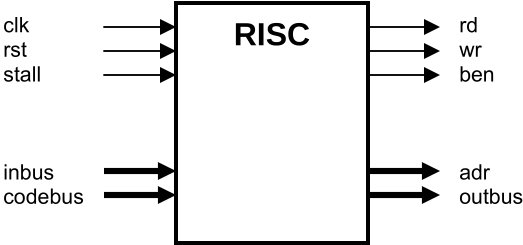
\includegraphics[width=.96\textwidth]{i/F/1.png}
	\caption{The processor's interface}
	\label{fig:processor}
\end{figure}

The main parts of the hardware interface are three busses, the data input and output busses, the
code bus, and the address bus. Signals $rd$ and $wr$ indicate, whether a read or a write operation is to
be performed. $ben$ indicates a byte (rather than word) access. The entire processor operates
synchronously on the clock $clk$ (25 MHz on Spartan-3), $rst$ is the reset signal (from a push button on
the development board), and $stall$ is the input to stall the processor.

First we concentrate on the implementation of the processor core, its realization in the form of
circuits. They are divided into two parts, the Arithmetic/Logic Unit(ALU) processing data, and the control
unit determining the flow of instructions.

\section{The arithmetic and logic unit}
The ALU features a bank of 16 registers with 32 bit words. Arithmetic and logical operations,
represented by instructions, always operate on these registers. Data can be transferred between
memory and registers by separate load and store instructions. This is an important characteristic of
RISC architectures, developed between 1975 and 1985. It contrasts with the earlier CISC
architectures (Complex Instruction Set): Memory is largely decoupled from the processor. A second
important characteristic is that most instructions take a single clock cycle (25 MHz) for their
execution. The exceptions are access to memory, multiplication and division. More about this will be
presented later. This single-cycle rule makes such processors predictable in performance. The
number of cycles and the time required for executing any instruction sequence is precisely defined.
Predictability is essential in all real-time applications.

\begin{figure}[h!]
	\centering
	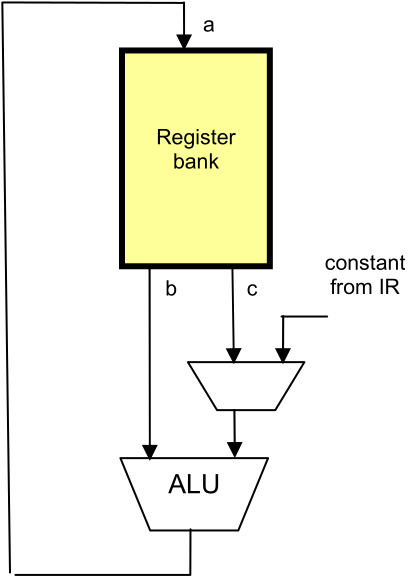
\includegraphics[width=.5\textwidth]{i/F/2.png}
	\caption{Processor core with ALU and registers}
	\label{fig:alu}
\end{figure}

The data processing unit consisting of ALU and registers is shown in Figure \ref{fig:alu}. Evidently, data
cycle from registers through the ALU, where an operation is performed, and the result is deposited
back into a register. The ALU embodies the circuits for arithmetic operations, logical operations,
and shifts. The operations available are listed below. They are described in more detail in
Appendix A2. The operand $n$ is either a register or a part of the instruction itself.

\begin{verbatim}
   0 MOV a,n   R.a:=n
   1 LSL a,b,n R.a:=R.b  ←  n (shift L by n bits)
   2 ASR a,b,n R.a:=R.b  →  n (shift R by n bits
                              with sign extension)
   3 ROR a,b,n R.a:=R.b rot n (rotate R by n bits)

   4 AND a,b,n R.a:=R.b  &  n (logical
   5 ANN a,b,n R.a:=R.b  & ~n  operations)
   6 IOR a,b,n R.a:=R.b  or n (inclusive or)
   7 XOR a,b,n R.a:=R.b xor n (exclusive or)

   8 ADD a,b,n R.a:=R.b  +  n (
   9 SUB a,b,n R.a:=R.b  –  n  integer
  10 MUL a,b,n R.a:=R.b  x  n  arithmetic
  11 DIV a,b,n R.a:=R.b div n )

  12 FAD a,b,c R.a:=R.b + R.c (
  13 FSB a,b,c R.a:=R.b – R.c  floating-point
  14 FML a,b,c R.a:=R.b x R.c  arithmetic
  15 FDV a,b,c R.a:=R.b / R.c )
\end{verbatim}

The following excerpt describes the essence of the ALU circuits. It is written in the HDL Verilog
and refers to the following wires and registers.

\begin{verbatim}
  wire [31:0] IR;  // instruction field(s):
  wire p, q, u, v, w;
      // IR[31], IR[30], IR[29], IR[28], IR[16]
  wire [3:0] op, ira, irb, irc;
      // IR[19:16], IR[27:24], IR[23:20], IR[3:0]
  wire [15:0] imm; // IR[15:0]

  wire [31:0] A, B, C0, C1, regmux;
  wire [31:0] s3, t3, quotient, fsum, fprod, fquot;
  wire [32:0] aluRes;
  wire [63:0] product;

  reg [31:0] R [0:15]; // array of 16 registers
  reg N, Z, C, OV;     // condition flags
\end{verbatim}

$B$ and $C0$ are the outputs from the register bank, and $A$ is its input. The register numbers $ira$ for port
$A$, $irb$ for port $B$, and $irc$ for port $C0$ are taken from 4-bit fields of the instruction register IR. $C1$ is the
multiplexer selecting among the register output $C0$ and the immediate field $imm$. $s3$ and $t3$ are
outputs of the shift units (Sect. 16.2.1). $product$ is the output of the multiplier (16.2.2), $quotient$ and
remainder those of the divider (16.2.3), $fsum$ that of the floating-point adder (16.2.4), $fprod$ that of the
floating-point multiplier (16.2.5), and $fquot$ the output of the floating-point divider (16.2.6).

\begin{verbatim}
  assign A  = R[ira];
  assign B  = R[irb];
  assign C0 = R[irc];
  assign C1 = q ? {{16{v}}, imm} : C0;
\end{verbatim}

The following represents the main instruction decoding and selection of results. The opcodes refer to
specific values of fields p and op of IR. Note that if $x$ then $y$ else $z$ is denoted in Verilog by $x ? y : z$.

\begin{verbatim}
  assign aluRes = MOV
    ? (q ? (~u ? {{16{v}}, imm}
               : {imm, 16'b0})
         : (~u ? C0
               : (~irc[0] ? H
                          : {N, Z, C, OV, 20'b0,
                             8'b01010000})))
    :  LSL  ? t3       // L-shift unit output
    : (ASR
      |ROR) ? s3       // R-shift unit output
    :  AND  ? B & C1
    :  ANN  ? B & ~C1
    :  IOR  ? B | C1
    :  XOR  ? B ^ C1
    :  ADD  ? B + C1 + (u & C)
    :  SUB  ? B - C1 - (u & C)
    :  MUL  ? product [31:0] // multiplier output
    :  DIV  ? quotient
    : (FAD
      |FSB) ? fsum
    :  FML  ? fprod
    :  FDV  ? fquot : 0;
\end{verbatim}

The input to the register bank, $regmux$, is selected from either $aluRes$, inbus (for LDR instructions),
or the program address $nxpc$ (for branch and link instructions). The signal $regwr$ determines,
whether data are to be stored (written) into the register bank. Details must be gathered from the
respective program listing RISC.v.

\begin{verbatim}
  always @ (posedge clk) begin
    R[ira] <= regwr     ?  regmux     : A ;
    N      <= regwr     ?  regmux[31] : N ;
    Z      <= regwr     ? (regmux==0) : Z ;
    C      <= (ADD|SUB) ?  aluRes[32] : C ;
    OV     <= (ADD|SUB) ?  aluRes[32]
                         ^ aluRes[31] : OV;
  end
\end{verbatim}

Whenever a register is written, the condition flags are also affected. They are $N$ ($aluRes$ negative),
$Z$ ($aluRes$ zero), $C$ (carry), and $OV$ (overflow). The latter apply only to addition and subtraction.

\subsection{Shifters}
Shifters are multi-way multiplexers. For a 32-bit word, the simplest solution would be 32 32-way
multiplexers. But this is hardly economical. On the FPGA used here, 4-way muxes are basic cells.
It is therefore beneficial, to compose a shifter out of 4-way muxes. Now the obvious solution is to
use 3 levels of muxes through which data flow. The first level shifts by amounts of 0, 1, 2, or 3, the
second by amounts of 0, 4, 8, 12, and the third by 0 or 16. This scheme is programmed as follows
for left shifts (instruction LSL) with $B$ as input, $sc0 = C1[1:0]$ and $sc1 = C1[3:2]$ as shift counts, and
$t3$ as output:

\begin{verbatim}
  assign t1 = (sc0 == 3) ? { B[28:0],  3'b0} :
              (sc0 == 2) ? { B[29:0],  2'b0} :
              (sc0 == 1) ? { B[30:0],  1'b0} : B ;
  assign t2 = (sc1 == 3) ? {t1[19:0], 12'b0} :
              (sc1 == 2) ? {t1[23:0],  8'b0} :
              (sc1 == 1) ? {t1[27:0],  4'b0} : t1;
  assign t3 =   C1[4]    ? {t2[15:0], 16'b0} : t2;
\end{verbatim}

The solution for right shifts is analogous. An additional level of multiplexing is required, shifting in
either the sign bit (ASR with sign propagation) or bits from the low end of the word (ROR), making
a barrel shifter. This selection is controlled by the instruction bit $w = IR[16]$.

\subsection{Multiplication}
Multiplication is an inherently more complex operation than addition and subtraction. After all,
multiplication can be composed (of a sequence) of additions. There are many methods to
implement multiplication, all – of course – based on the same concept of a series of additions.
They show the fundamental problem of trade-off between time and space (circuitry). Some
solutions operate with a minimum of circuitry, namely a single adder used for all 32 additions
executed sequentially (in time). They obviously sacrifice speed. The other extreme is multiplication
in a single cycle, using 32 adders in series (in space). This solution is fast, but the amount of
required circuitry is high.

Before we present the sequential solution, let us briefly recapitulate the basics of a multiplication $p
:= x × y$. Here $p$ is the product, $x$ the multiplier, and $y$ the multiplicand. Let $x$ and $y$ be unsigned
integers. Consider $x$ in binary form.

\[  x = x_{31}×2^{31} + x_{30}×2^{30} + … + x_1×2^1 + x_0×2^0 \]

Evidently, the product is the sum of 32 terms of the form $x_k×2^k×y$, i.e. of $y$ left shifted by $k$ positions
multiplied by $x_k$. Since $x_k$ is either $0$ or $1$, the product is either $0$ or $y$ (shifted). Multiplication is thus
performed by an adder and a selector. The selector is controlled by $x_k$, a bit of the multiplier.
Instead of selecting this bit among $x_0$ … $x_{31}$, we right shift $x$ by one bit in each step. Then the
selection is always according to $x_0$. The add-shift step then is 
\begin{verbatim}
  IF ODD(x) THEN p := p + y END;
  y := 2*y; x := x DIV 2
\end{verbatim}

whereby multiplication by 2 is done by a left shift, and division by 2 by a right shift: As an example,
consider the multiplication of two 4-bit integers $x = 5$ and $y = 3$, requiring 4 steps:
\begin{table}[h!]
  \centering
  \begin{tabular}{l l l l l}
               & p         & x    & y         \\\hline
               & 0000'0000 & 0101 & 0000'0011 \\
    add y to p & 0000'0011 & 0101 & 0000'0011 \\
    shift      & 0000'0011 & 0010 & 0000'0110 \\
    add 0 to p & 0000'0011 & 0010 & 0000'0110 \\
    shift      & 0000'0011 & 0001 & 0000'1100 \\
    add y to p & 0000'1111 & 0001 & 0000'1100 \\
    shift      & 0000'1111 & 0000 & 0001'1000 \\
    add 0 to p & 0000'1111 & 0000 & 0001'1000 \\
    shift      & 0000'1111 & 0000 & 0011'0000 & p = 15
  \end{tabular}
\end{table}

The shifting of $x$ to the right also suggests that instead of shifting $y$ to the left in each step, we
keep $y$ in the same position and shift the partial sum $p$ to the right. We notice that the size of $x$
decreases by 1 in each step, whereas the size of $p$ increases by 1. This allows to pack $p$ and $x$
into a single double register <$B$, $A$> with a shifting border line. At the end, it contains the product $p
= x × y$.

\begin{table}[h!]
  \centering
  \begin{tabular}{l l r l}
               & p        &    x \\\hline
               & 0000     & 0101 \\
    add y to p & 0011     & 0101 \\
    shift      & 00011    &  010 \\
    add 0 to p & 00011    &  010 \\
    shift      & 000011   &   01 \\
    add y to p & 001111   &   01 \\
    shift      & 0001111  &    0 \\
    add 0 to p & 0001111  &    0 \\
    shift      & 00001111 &      & p = 15
  \end{tabular}
\end{table}
\begin{verbatim}
  p = {B[31:0], A{31:[32-k]},
  x = A[31-k:0]               k = 0 … 31
\end{verbatim}

The multiplier is controlled by a rudimentary state machine $S$, actually a simple 5-bit counter
running from 0 to 31. The multiplier is shown schematically in Figure \ref{fig:multiplier}.

\begin{figure}[h!]
	\centering
	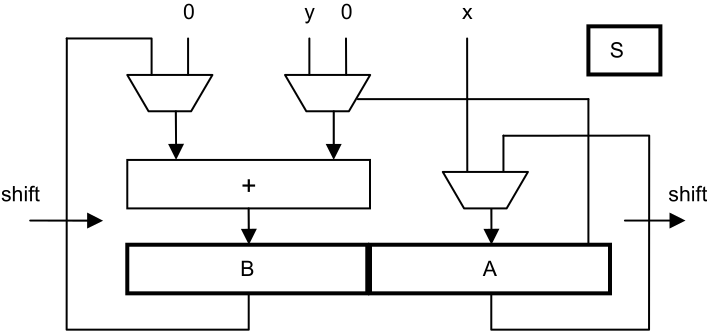
\includegraphics[width=.9\textwidth]{i/F/3.png}
	\caption{Schematic of multiplier}
	\label{fig:multiplier}
\end{figure}

The multiplier interprets its operands as signed ($u = 0$) or unsigned ($u = 1$) integers. The difference
between unsigned and signed representation is that in the former case the first term has a
negative weight ($-x_{31}×2^{31}$). Therefore, implementation of signed multiplication requires very little
change: Term 31 is subtracted instead of added (see complete program listing below).

\begin{verbatim}
  stall = MUL & ~(S == 31);
  S <= MUL ? S+1 : 0;
\end{verbatim}

During execution of the 32 add-shift steps the processor must be stalled. The process proceeds
and the counter $S$ advances as long as the input MUL is active (high). MUL indicates that the
current operation is a multiplication, and the signal is stable until the processor advances to the
next instruction. This happens when step 31 is reached (Figure \ref{fig:stall}).

\begin{figure}[h!]
	\centering
	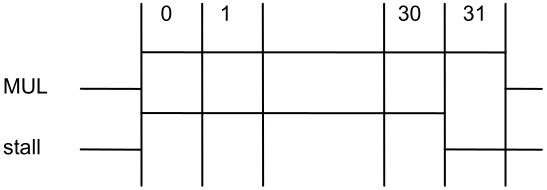
\includegraphics[width=.9\textwidth]{i/F/4.png}
	\caption{Generating $stall$}
	\label{fig:stall}
\end{figure}

The details of the simple multiplier are listed below:

\begin{verbatim}
  module Multiplier(
    input CLK, MUL, u,
    output stall,
    input [31:0] x, y,
    output [63:0] z);
 
  reg [4:0] S; // state
  reg [31:0] B2, A2; // high and low parts of partial product
  wire [32:0] B0, B00, B01;
  wire [31:0] B1, A0, A1;
 
  assign stall = MUL & ~(S == 31);
  assign B00 = (S == 0) ? 0 : {B2[31] & u, B2};
  assign B01 = A0[0] ? {y[31] & u, y} : 0;
  assign B0 = ((S == 31) & u) ? B00 - B01 : B00 + B01;
  assign B1 = B0[32:1];
  assign A0 = (S == 0) ? x : A2;
  assign A1 = {B0[0], A0[31:1]};
  assign z = {B1, A1};
 
  always @ (posedge(CLK)) begin
    B2 <= B1; A2 <= A1;
    S <= MUL ? S+1 : 0;
  end
  endmodule
\end{verbatim}

Implementing multiplication in hardware made the operation about 30 times faster than its solution
by software. A significant factor! As multiplication is a relatively rare operation – at least in
comparison with addition and subtraction – early RISC designs (MIPS, SPARC, ARM) refrained
from its full implementation in hardware. Instead, an instruction called multiply step was provided,
performing a single add-shift step in one clock cycle. A multiplication was then programmed by a
sequence of 32 step instructions, typically provided as a subroutine. This measure of economy
was abandoned, when hardware became faster and cheaper.

The FPGA used on the Spartan-3 board features a welcome facility for speeding up multiplication,
namely fast 18 x 18 bit multiplier units. These are made available as basic cells of the FPGA, and
they multiply in a single clock cycle. Considering an operand $x = x_1×2^{16} + x_0$, the product is
obtained as the sum of only 4 terms:

\[ p = x × y = x_1×y_1×2^{32} + (x_0×y_1 + x_1×y_0)×2^{16} + x_0×y_0 \]

Thereby multiplication of two 32-bit integers can be performed in 2 cycles only, one for
multiplications, one for addition. Four multipliers are needed. For details, the reader is referred to
the program listing (module Multiplier1).

\subsection{Division}
Division is similar to multiplication in structure, but slightly more complicated. We present its
implementation by a sequence of 32 shift-subtract steps, the complement of add-shift. We here
discuss division of unsigned integers only.

\begin{verbatim}
  q = x DIV y
  r = x MOD y
\end{verbatim}

$q$ is the quotient, $r$ the remainder. These are defined by the invariants

\[ x = q×y + r\text{ with }0 \le r < y \]

Both $q$ and $r$ are held in registers. Initially we set $r$ to $x$, the dividend, and then subtract multiples
of $y$ (the divisor) from it, each time checking that the result is not negative. This shift-subtract step is

\begin{verbatim}
  r := 2*r; q := 2*q;
  IF r – y >= 0 THEN r := r – y END
\end{verbatim}

As an example, consider the division of the 8-bit integer $x = 14$ by the 4-bit integer $y = 4$, where
multiplication and division by 2 are done by shifts:

\begin{table}[h!]
  \centering
  \begin{tabular}{l l l l l}
                 & r         & q    & y         \\\hline
                 & 0000'1110 & 0000 & 0001'1000 \\
    shift        & 0000'1110 & 0000 & 0001'1000 & r < y \\
    sub 0 from r & 0000'1110 & 0000 & 0000'1100 \\ 
    shift        & 0000'1110 & 0000 & 0000'1100 & r >= y \\
    sub y from r & 0000'0010 & 0001 & 0000'1100 \\ 
    shift        & 0000'0010 & 0010 & 0000'0110 & r < y \\
    sub 0 from r & 0000'0010 & 0010 & 0000'0110 \\ 
    shift        & 0000'0010 & 0100 & 0000'0011 & r < y \\
    sub y from r & 0000'0010 & 0100 & 0000'0011 & q = 4, r = 2
  \end{tabular}
\end{table}

As with multiplication this arrangement may be simplified by putting r and q into a double-length
shift register, and by shifting r to the left instead of y to the right. This results in

\begin{table}[h!]
  \centering
  \begin{tabular}{l l r l}
                 & r         &    q \\\hline
                 & 0000'1110 &      \\
    shift        & 0001'110  &    0 & r < Y \\
    sub 0 from r & 0001'110  &    0 \\
    shift        & 0011'10   &   00 & r >= Y \\
    sub y from r & 0000'10   &   01 \\
    shift        & 0001'0    &  010 & r < Y \\
    sub 0 from r & 0001'0    &  010 \\
    shift        & 0010      & 0100 & r < Y \\
    sub 0 from r & 0010      & 0100 & q = 4, r = 2
  \end{tabular}
\end{table}

This scheme is represented by the circuit shown in Figure \ref{fig:divider}.

\begin{figure}[h!]
	\centering
	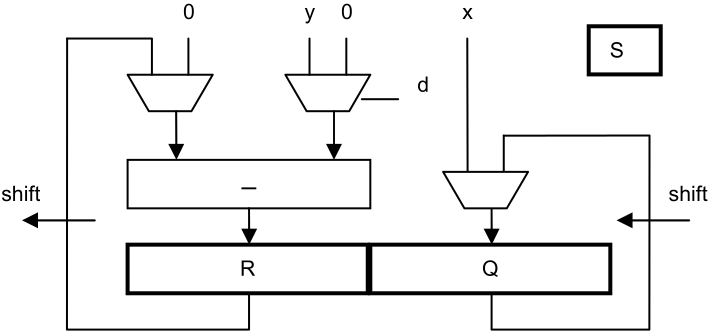
\includegraphics[width=.9\textwidth]{i/F/5.png}
	\caption{Schematic of divider}
	\label{fig:divider}
\end{figure}

Stall generation is the same as for the multiplier. A division takes 32 clock cycles. Further details
are shown in the subsequent program listing.

\begin{verbatim}
  module Divider(
    input clk, DIV,
    output stall,
    input [31:0] x, y,
    output [31:0] quot, rem);
 
  reg [4:0] S; // state
  reg [31:0] r3, q2;
  wire [31:0] r0, r1, r2, q0, q1, d;
 
  assign stall = DIV & ~(S == 31);
  assign r0 = (S == 0) ? 0 : r3;
  assign d = r1 - y;
  assign r1 = {r0[30:0], q0[31]};
  assign r2 = d[31] ? r1 : d;
  assign q0 = (S == 0) ? x : q2;
  assign q1 = {q0[30:0], ~d[31]};
  assign rem = r2;
  assign quot = q1;
  
  always @ (posedge(clk)) begin
    r3 <= r2; q2 <= q1;
    S <= DIV ? S+1 : 0;
  end
  endmodule
\end{verbatim}

\section{Floating-point arithmetic}
The RISC uses the IEEE Standard for representing REAL (floating-point) numbers with 32 bits.
The word is divided into 3 fields: s for the sign, e for the exponent, and m for the mantissa. The
value is 

\[ x = (-1)^s × 2^{-127} × 1.m\text{ with }1.0 \le m < 2.0\text{ (normalized form)} \]

Numbers are represented in sign-magnitude form. This implies that for sign inversion only the sign
bit must be inverted, and exponent and mantissa remain unchanged.

Zero is a special case represented by 32 0-bits, and therefore has to be treated separately.
Furthermore, e = 255 denotes "not a number". It is generated in the case of arithmetic overflow.

\begin{figure}[h!]
	\centering
	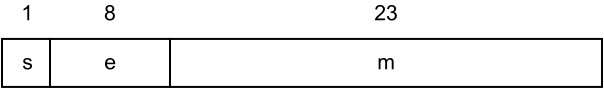
\includegraphics[width=.9\textwidth]{i/F/6.png}
	\caption{IEEE standard floating-point representation of REAL numbers}
	\label{fig:float-point}
\end{figure}

\subsection{Floating-point addition}
If two numbers are to be added, they must have the same exponent. This implies that the
summand with the smaller exponent must be denormalized. m is shifted to the right and e is
incremented accordingly. That is, if d is the difference of the two exponents, m is multiplied by 2d,
and e is incremented by d. After the addition, the sum must be rounded and post-normalized. m is
shifted to the left and e is decremented accordingly. The shift amount is determined by the
position of the leftmost one-bit. This results in the scheme shown in Figure 16.7, and the module's
interface is

\begin{verbatim}
  module FPAdder(
    input clk, run, u, v,
    input [31:0] x, y,
    output stall,
    output [31:0] z);
\end{verbatim}
\begin{figure}[h!]
	\centering
	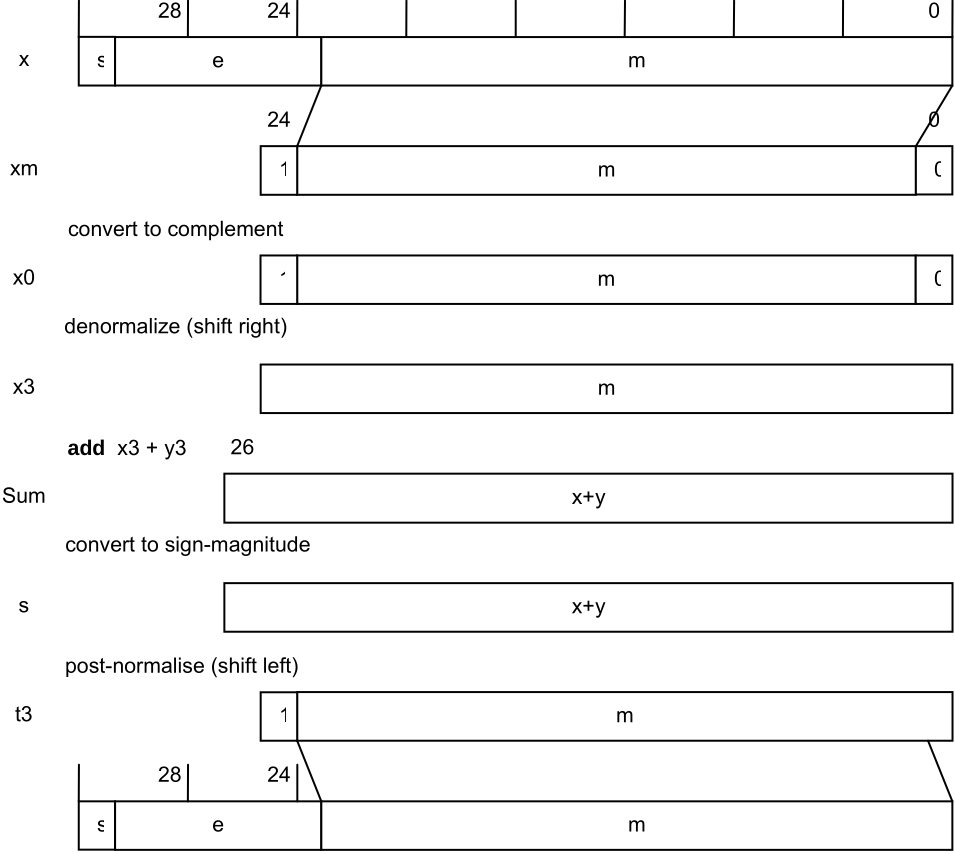
\includegraphics[width=.9\textwidth]{i/F/7.png}
	\caption{Steps of floating-point addition}
	\label{fig:fpaddition}
\end{figure}

It is important to achieve proper rounding. This is done by extending the mantissa of both
operands by a guard bit, initialized to 0. A one is added (effectively 0.5) and at the end the guard
bit is discarded.

The two predefined conversion functions FLT and FLOOR are conveniently implemented as
additions. A denormalized 0 is added to the argument, effecting the proper shift. In the case of
FLT (modifier bit u = 1), denormalization is omitted (no 1-bit inserted), and in the case of FLOOR
(modifier bit v = 1), post-normalization is suppressed.

\subsection{Floating-point multiplication}
A product is given by the equation

\[ p = x × y = (2^{xe} × xm) × (2^{ye} × ym) = 2^{xe+ye} × (xm * ym) \]
\[ p = (xs, xe, xm) × (ys, ye, ym) = (xs\text{ xor }ys, xe + ye, xm × ym) \]

That is, exponents are added, mantissas multiplied. Denormalization is not needed. Post-
normalization is a right shift of at most one bit, because if 1.0 $\le$ xm, ym < 2.0, the result satisfies
1.0 $\le$ xm*ym < 4.0. The sign of the product is the exclusive or of the signs of the arguments. The
multiplier module's interface is

\begin{verbatim}
  module FPMultiplier(
    input clk, run,
    input [31:0] x, y,
    output stall,
    output [31:0] z);
\end{verbatim}

\subsection{Floating-point division}
A quotient is given by the equation

\begin{verbatim}
  module FPDivider(
    input clk, run,
    input [31:0] x, y,
    output stall,
    output [31:0] z);
\end{verbatim}

\section{The Control Unit}
\[ q = x / y = (2^{xe} × xm) / (2^{ye} × ym) = 2^{xe-ye} × (xm / ym) \]
\[ q = (sx, ex, mx) / (sy, ey, my) = (sx\text{ xor }sy, ex - ey, mx / my) \]

That is, exponents are subtracted, mantissas divided. Denormalization is not needed. Post-
normalization requires a left shift by at most a single bit, because if $1.0 \le xm, ym < 2.0$, the result
satisfies $0.5 \le xm/ym < 2.0$. The sign of the product is the exclusive or of the signs of the
arguments. The divider module's interfaces is

The control unit determines the sequence of executed instructions. It contains two registers, the
program counter PC holding the address of the current instruction, and the current instruction
register IR holding the instruction currently being interpreted. Instructions are obtained from
memory through the codebus (see interface), from where the decoding signals emanate. Mostly,
the arithmetic unit and the control unit operate concurrently (in parallel). While the arithmetic unit
performs the operation held in register IR and data signals flow through the ALU, the control unit
fetches in the same clock cycle the next instruction from memory in the location with the address
held in PC. Next address and next instruction are latched in the registers at the end of a cycle.
This scheme constitutes a one-element pipeline of instructions.

The principal task of the control unit is to generate the address of the next instruction. There are
essentially only four cases:

\begin{enumerate}
  \item Zero on reset.
  \item The next instructions address is PC+1 (all instructions except branches)
  \item The branch target PC+1 + offset. (Branch instructions).
  \item It is taken from a data register. (This is used for returning from procedures).
\end{enumerate}

This is reflected by the following program text, and shown in Figure \ref{fig:cu}.

\begin{figure}[h!]
	\centering
	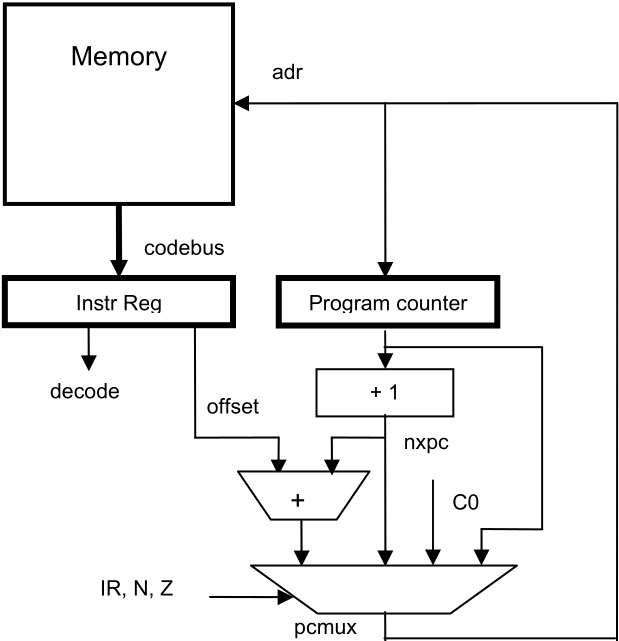
\includegraphics[width=.9\textwidth]{i/F/8.png}
	\caption{The control unit}
	\label{fig:cu}
\end{figure}

\begin{verbatim}
  reg [17:0] PC;
  reg [31:0] IRBuf;
  wire [31:0] IR;
  wire [31:0] pmout;
  wire [17:0] pcmux, nxpc;
  wire cond;
 
  IR = codebus;
  nxpc = PC + 1;
  pcmux = (~rst) ? 0 :
      (stall) ? PC : // stall
      (BR & cond & u) ? off + nxpc :
      (BR & cond & ~u) ? C0[19:2] :
      nxpc;
 
  always @ (posedge clk) PC <= pcmux; end
\end{verbatim}

Branches are the only conditional instructions. Whether a branch is taken or not, is determined by
the combination of the condition flags selected by the condition code field of the branch
instruction. IR[27] is the condition sense inversion bit.

\begin{verbatim}
  reg N, Z, C, OV; // condition flags
  wire S;
  assign S = N ^ OV;
  assign cond = IR[27] ^
      ((cc == 0) &   N   |  // MI, PL
       (cc == 1) &   Z   |  // EQ, NE
       (cc == 2) &   C   |  // CS, CC
       (cc == 3) &  OV   |  // VS, VC
       (cc == 4) & (C|Z) |  // LS, HI
       (cc == 5) &   S   |  // LT, GE
       (cc == 6) & (S|Z) |  // LE, GT
       (cc == 7));          //  T, F
\end{verbatim}

There is, unfortunately, a complication obfuscating the simple scheme presented so far. It stems
from the necessity to initialize the processor. Only registers and memory blocks (BRAM) can be
initialized and loaded by the available FPGA-tools. How, then, is a program (in our case the boot
loader) moved into memory, the chip-external SRAM? The following scheme has been chosen:

The initial program is loaded into a BRAM (1K x 32). This block is memory-mapped into high-end
addresses in the range of the data stack. On startup, the flag PMsel is set and IR is loaded from
pmout (from the BRAM) at StartAdr. At the end of the program (boot loader), a branch instruction
with destination 0 jumps to the beginning of the program that had just been loaded into SRAM by
the boot loader. This is, presumably, but not necessarily, the operating system. The following
changes and additions are required:

\begin{verbatim}
  localparam StartAdr = 18'b111111100000000000; // 0FE000H

  reg PMsel; // memory select for instruction fetch
  reg [31:0] IRBuf;

  dbram32 PM ( // BRAM
      .clka (clk),
      .rdb (pmout), // output port
      .ab (pcmux[10:0])); // address

  assign IR = PMsel ? pmout : IRBuf;

  always @ (posedge clk) begin
    PMsel <= ~rst | (pcmux[17:11] == 7'b1111111);
    IRBuf <= stall ? IRBuf : codebus;
    ...
  end;
\end{verbatim}

%\chapter{Dynamic Data Structures and Pointers}
\label{ch:ptr}
Array and record structures share the common property that they are static. This implies
that variables of such a structure maintain the same structure during the whole time of
their existence.  In many applications, this is an intolerable restriction; they require
data which do not only change their value, but also their composition, size, and structure.
Typical examples are lists and trees that grow and shrink dynamically. Instead of providing
list and tree structures, a collection that for some applications would again not suffice,
Oberon offers a basic tool to construct arbitrary structures.  This is the pointer type.

Every complex data structure ultimately consists of elements whose structure is static.
Pointers, i.e. values of pointer types, are themselves not structured, but rather are used
to establish relationships among those static elements, usually called \emph{nodes}. We
also say that pointers link elements or point to elements. Evidently, different pointer
variables may point to the same element, hence providing the possibility to compose
arbitrarily complex structures, and at the same time opening many pitfalls for programming
mistakes that are difficult to pinpoint. Operating with pointers indeed requires utmost care.

Pointers in Oberon cannot point to arbitrary variables. The type of variable to which they
point must be specified in the pointer type's declaration, and the pointer type is said to
be bound to the referenced object's type. Example:
\begin{verbatim}
  TYPE Node = POINTER TO NodeDescriptor
  VAR p0, p1: Node
\end{verbatim}
Here Node (and thereby also variables \verb|p0| and \verb|p1|) are bound to the type
\verb|NodeDescriptor|, i.e. they can point to variables of type \verb|NodeDescriptor| only.
These variables, typically of record type, are not created by the declaration of \verb|p0|
and \verb|p1|. Instead, they are created by an allocation procedure call. In Oberon, it is
represented by a predefined operator called \verb|NEW|. The statement \verb|NEW(p0)| then
creates a (record) variable of type \verb|NodeDescriptor| and assigns a pointer referring
to that variable (i.e. a value of type \verb|Node|) to \verb|p0|. The created variable is
said to be dynamically created (allocated); it has no name, is anonymous, and can be accessed
only via a pointer using the dereferencing operator \^{}. The said variable is denoted by
the designator \verb|p0^|. If the referenced variable is of record type with, say, fields
$x$ and $y$, then the fileds are denoted, for example, by \verb|p0^.x, p1^.y|.  Since in
this case it is clear that field selection applies to the referenced record rather than to
the pointer, the designators may be abbreviated into \verb|p0.x| and \verb|p1.y|.
\begin{verbatim}
  PointerType = POINTER TO type.
\end{verbatim}
What really makes pointers such a powerful tool is the circumstance that they may point to
variables which themselves contain pointers. This reminds us of procedures that call procedures
and thereby introduce recursion. In fact, pointers are the tool to implement recursively
defined data structures (such as lists and trees). The nature of the recursive data structure
is evident from the declaration of the type of its elements.

Just as every recursion of procedure activation must terminate at some time, so must every
recursion in referencing terminate at some point. The role of the if statement to terminate
procedural recursion is here taken by the special pointer value \verb|NIL| terminating
referencing recursion. \verb|NIL| points to no object. It is an obvious consequence that a
designator of the form \verb|p^ (p^.x, p.x)| must never be evaluated, if \verb|p = NIL|.
We summarize the following essential points:
\begin{enumerate}
  \item Every pointer type is bound to a type; its values are pointers which point to
    variables of that type.
  \item The referenced variables are anonymous and can be accessed via pointers only.
  \item The referenced variables are dynamically created by an allocation procedure which
    assigns the variable's pointer to $p$.
  \item The pointer constant \verb|NIL| belongs to every pointer type and points to no object.
  \item The variable referenced by a pointer $p$ is denoted by the designator \verb|p^|.
    In order for \verb|p^| to be meaningful, $p$ must not have the value \verb|NIL|.
  \item Field designators of the form \verb|p^.x| may be abbreviated to \verb|p.x|.
\end{enumerate}
Lists, also called linear lists or chains, are characterized by consisting of record typed
nodes that each have exactly 1 element being a pointer to a record of the same type as itself.
This implies recursion. A list pointer declaration then assumes the characteristic form
\begin{verbatim}
  List = POINTER TO ListDesc;
  ListDesc = RECORD key: INT;
                    Data: ...
                    next: List
             END
\end{verbatim}
"Data" actually stands for any number of fields representing data pertaining to the listed
node.  Key is part of these data; it is mentioned separately here because it is quite common
to associate with each element a unique identifying key, and also because it will be used
in subsequent examples of operations on lists. The essential ingredient here, however, is
the field \verb|next|, so labelled because it evidently is the pointer to the next element
in the list. Direct recursion in data type declarations is not permitted for the obvious
reason that there would be no evident termination. The declaration given above can NOT be
abbreviated into
\begin{verbatim}
  List = RECORD key: INT; next: List END
\end{verbatim}
Assume now that a list is accessible in a program via its 1st element, denoted by the
pointer variable
\begin{verbatim}
  first: List
\end{verbatim}
The empty list is represented by \verb|first = NIL|. A non-empty list is most conveniently
constructed by inserting new elements at its front. The following assignments are needed
to insert one element (let $p$ be an auxiliary variable of type \verb|List|)
\begin{verbatim}
  NEW(p); (*assign values to p.key and p.data*)
  p.next := first; first := p
\end{verbatim}
Having constructed a list by repeated insertion of nodes, we may wish to search the list
for a node with key value equal to a given $x$. We evidently use a repetition; the while
statement is appropriate, because we do not know the number of nodes (and hence repetitions)
beforehand. It is wise to include the case of the empty list!
\begin{verbatim}
  p := first;
  WHILE (p # NIL) & (p.key # x) DO
    p := p.next
  END;
  IF p # NIL THEN found END
\end{verbatim}
We draw attention to the fact that here we make use of the rule that the term $b$ is not
evaluated, if in the expression \verb|a & b|, the factor $a$ is found to be \verb|FALSE|.
If this rule would not hold, the factor \verb|p.key # x| might be evaluated with
\verb|p = NIL|, which is illegal.

The 2nd frequently encountered dynamic data structure is the tree. It is characterized by
its nodes having $n$ pointer fields each, where $n$ is the degree of the tree. The common
and in some sense optimal case is the binary tree with $n = 2$. Lists now appear as
degenerate trees of degree 1.  The respective declarations are
\begin{verbatim}
  Tree = POINTER TO TreeNode;
  TreeNode = RECORD key: INT:
                   data: ...
                   left,
                  right: Tree
             END
\end{verbatim}
The place of the variable \verb|first| in the case of lists is taken by a variable to be
\begin{verbatim}
  root: Tree
\end{verbatim}
with \verb|root = NIL| denoting the empty tree. Trees are commonly used to represent
collections of data in order of ascending key values, making retrieval very efficient.
The following statements represent a search in an ordered binary tree, whose similarity
to the binary search in an ordered array is remarkable. Again, $p$ is an auxiliary
variable (of type \verb|Tree|).
\begin{verbatim}
  p := root:
  WHILE (p # NIL) & (p.key # x) DO
    IF p.key <x THEN p := p.right
                ELSE p := p.left END
  END;
  IF p # NIL THEN found END
\end{verbatim}
This example is a repetitive version of the tree search. Next we show the recursive version.
It is, in addition, extended such that a new node is created and inserted at the appropriate
place, whenever no node with key value $x$ exists.
\begin{verbatim}
  PROC search(VAR p: Tree; x: INT): Tree;
    VAR q: Tree;
  BEGIN
    IF p # NIL THEN
      IF p.key < x THEN
        q := search(p.right, x)
      ELSIF p.key > x THEN
        q := search(p^.left, x)
      ELSE
        q := p
      END
    ELSE (*not found, hence insert*)
      NEW(q); q.key := x;
      q.left:= NIL; q.right := NIL
    END;
    RETURN q
  END search
\end{verbatim}
The call \verb|search(root, x)| now stands for a search of $x$ in the tree represented by
the variable \verb|root|.

And this concludes our examples of operations on lists and trees to illustrate pointer
handling. Lists and trees have nodes which are all of the same type. We draw attention to
the fact that the pointer facility admits the construction of even more general data
structures consisting of nodes of various types. Typical for all these structures is that
all nodes are declared as record types. Hence, the record emerges as a particularly useful
data structure in conjunction with pointers.

Creation of nodes is expressed by the standard procedure \verb|NEW|, which is part of a
system's storage management. We assume that retrieval of storage is performed automatically
by a so-called storage reclamation mechanism, also called \emph{garbage collector}. It
relies on the fact that records that are no longer referenced by any pointer may be
recollected, i.e. their storage can be recycled.

%\appendix
%\part*{Spec}
%\section{Oberon: Result of Simplification}
This brings us into the 1990 years. I felt that continued complexification had
reached an alarming state. To curtail this cancerous growth had become more and
more urgent, as systems had reached a size and weight under which they might
soon collapse, as nobody would fully understand these monsters, but rather
equate complex with powerful.

Reduction of complexity was the guiding principle behind the design of the
language Oberon . Quite obviously, Modula-2 was too complicated, and therefore
laborious to implement. Also, it had not quite reached the goal of being truly
computer-independent, a prerequisite for any language that claimed to be
"higher-level". Oberon marked a significant step towards this difficult, but crucial
and unique goal. The key to achieving it was the rigorous restriction to essential
features, and the discarding of all "bells and whistles", a genuine exercise towards
simplicity. But despite frugality, Oberon was to be a powerful, general-purpose
language in the tradition of Pascal and Modula. The result was a surprisingly small
language (which, in 2007) was revised again to become even more frugal.

This guideline, however, was not just an esoteric idea. It was a necessity. It was
decided to implement not only a compiler, but also an entire, self-contained
operating system along the lines of Cedar, existing at the Xerox PARC facility in
Palo Alto, a system that marked a radical departure from conventional,
batch-processing systems.Oberon was to be catering for full interactivity with a
high-resolution, bit-mapped display and a mouse. Compiler and operating system were
implemented by 2 people only (J. Gutknecht and me) in their spare-time over almost
2 years. Naturally, we were forced to concentrate on what was considered essential.
The successful implementation of the entire system in its own language proved that
the remaining features were sufficient, and that actually a simple language is more
suitable for a complex system than one which is part of the problem rather than of
the solution.

However, a single feature not present in Modula was added to Oberon: Type Extension.
The Algol - Modula line represents static typing. The type of a constant, variable,
or function is visible from the program text alone, without executing the program.
Type inconsistencies can therefore always be checked by the compiler. This rigid
scheme was to be slightly relaxed. Through type extension it becomes possible to
declare hierarchies of types, and to construct at run-time data structures with
elements of different, although related types. This is the key to object-oriented
programs; Oberon contains all the ingredients for object-oriented programming, but
no more. Type checking at run-time could be realized very efficiently.

Object-orientation had become the one popular innovation in the realm of software.
It had taken a long time since its origin was laid by the language Simula (Dahl \&
Nygaard) in 1967. It became better known (in the US) by the languages Smalltalk
(Kay) in 1976 (implemented on the Alto), and Object-Pascal (Tesler, 1980).
Smalltalk went all the way: everything was to be an object. You cannot add two
numbers $x$ and $y$. The proper way of looking at this problem is to consider $x$
as an object which contains a method to add $y$ to itself. Genius or perversion?

In 1995 Sun Microsystems presented its language Java, fully 6 years after Oberon.
It incorporated much of the "philosophy" of Oberon, but, alas, chose the style and
syntax of C. Around 2000 Microsoft released its language C\# as a strong competitor
of Java, and Google followed in 2007 with its language Go, even more strongly
following (the 18 years old) Oberon. The crux with these languages, which all became
wide-spread due to strong industrial support, is their size and complexity. The
ambition to provide everything to everybody prevailed and let them grow into complex
bodies difficult to master.

On the hardware front, the development was similar. The multitude of processor
architectures of earlier decades has vanished. Only a few architectures prevail,
mainly those of Intel and ARM. Engineers are pushed to make use of the abundance of
available transistors. One way is to provide several, even many, processors on the
same chip, another to include large cache memories, and yet another to provide
interfaces to external devices, such as to networks, or digital to analog and analog
to digital converters. Also here complexity grows without bounds. It becomes harder
and harder to recognize the original core and to identify the basic principles among
the myriad of gadgets and gismos.

The unbelievable success of computers is mostly due to the incredible advances in
semiconductor fabrication. Processors are now available with immense power, and
memories with vast capacity. As in every other field of endeavor, abundance at low
cost invariably leads to wasteful design. This entails not only waste, but poor
products of declining quality. In particular software engineering now seems to be
the El Dorado of splashing and wastefulness.

Dijkstra once claimed that it is the foremost duty of the software engineer to fight
(home-grown) complexity like the devil every minute. The same is now true also for
the hardware engineer.

%\chapter{Syntax of Oberon}
\begin{verbatim}
  digit  = 0-9
  hexdig = digit|A-F
  letter = A-Z|a-z
 
  id     = letter{letter|digit}
  qid    = [id.]id
  xid    = id[*]
 
  dec    = digit{digit}
  hex    = digit{hexdig}
  int    = dec | hex H
  sign   = +|-
  real   = [sign]dec.{digit}[E[sign]dec]
  number = int|real
  string = " {char} " | hex X
 
  const  = xid=expr
 
  typdef = xid=type
  type   = pre | arr | rec | ptr | pro | fun
  pre    = BOOL|BYTE|CHAR|INT|REAL|SET
  arr    = ARRAY len{, len} OF type
  len    = expr
  rec    = RECORD[ (base)][ fields] END
  base   = qid
  fields = field{; field}
  field  = xids: type
  xids   = xid{, xid}
  ptr    = POINTER TO type
  pro    = PROC[ params]
  fun    = PROC[ params]: qid
 
  expr   = exp [rel exp]
  rel    = =|#|<|<=|>|>=|IN|IS
  exp    = [sign]term {add term}
  add    = sign|OR
  term   = factor {mul factor}
  mul    = *|/|DIV|MOD|&
  factor = number | string | NIL | TRUE | FALSE
           | set | pc | (expr) | ~factor
  des    = qid{sel}
  sel    = .id|'['exprs']'|^|(qid)
  set    = '{' [seg{, seg}] '}'
  seg    = expr[..expr]
  exprs  = expr{, expr}
  args   = ([exprs])
 
  s      = [assign|pc|if|cases|while|repeat|for]
  assign = des:=expr
  pc     = des[args]
  ss     = s{; s}
  if     =     IF expr THEN ss
           {ELSIF expr THEN ss}
                      [ELSE ss] END
  cases  = CASE expr OF case {'|' case} END
  case   = [ranges: ss]
  ranges = range{, range}
  range  = label[..label]
  label  = int|string|qid
  while  = WHILE expr DO ss {ELSIF expr DO ss} END
  repeat = REPEAT ss UNTIL expr
  for    = FOR id:=expr TO expr[ BY expr] DO ss END
 
  proc   = prop | func
  prop   = PROC xid [params]; decls
           [BEGIN ss] END id
  func   = PROC xid [params]: qid; decls
           [BEGIN ss] [RETURN expr] END id
  decls  = [CONST {const;}][TYPE {typdef;}][VAR {field;}]
           {proc;}
  params = ([param{; param}])
  param  = [VAR] id{, id}: {ARRAY OF} qid
 
  module = MODULE id;[ IMPORT import{, import};] decls
           [BEGIN ss] END id.
  import = id[:= id]
\end{verbatim}

%\printbibliography
\end{document}
